
%% The following is a directive for TeXShop to indicate the main file
%%!TEX root = ../../thesis.tex

\chapter{An inversion approach for subsurface injections}
\label{ch:inversion}

\section{Introduction}
The previous three chapters have focussed on understanding the physics of electromagnetics over conductive, permeable, steel-cased wells. In this chapter, we return to the goal of imaging subsurface injections through geophysical inversion. We view this as a time-lapse problem, in which one data set is obtained prior to the injection and second data set is obtained after the injection. The aim of the inversion, then, is to characterize the changes in the earth model due to the injection.

Time-lapse direct current (DC) resistivity, and in some cases electromagnetics (EM), is commonly used in the groundwater hydrology community. In particular, DC resistivity has been used, in salt-tracer experiments aimed at understanding groundwater flow (e.g. \cite{Slater2002, Kemna2002, Singha2005, Doetsch2012}) and for characterizing time-lapse vadose zone processes (e.g. \cite{Daily1992, Park1998, Binley2002}). Within the context of hydrogeophysics, typically multiple time-lapse surveys are conducted. A range of interpretation techniques have been applied. In terms of algorithmic complexity, the most straightforward approach is to invert each time-snapshot independently. The recovered models can then be differenced and the difference interpreted \citep{Cassiani2006}, or an intermediate interpretation, for example estimating the center of mass of a plume \citep{Singha2006, Doetsch2012}, can serve as an indicator that is tracked through time. \cite{Daily1992} presented an approach for inverting ratios between initial and subsequent datasets, and \citep{LaBrecque2000} proposed an inversion for the resistivity difference between two subsequent data sets by inverting the difference between the two data sets. A common approach is to use the inversion result from an initial timestep as a reference and starting model for the following datasets \citep{Loke2001, Oldenborger2007}, this is sometimes referred to as a ``cascaded inversion'' \citep{Miller2008}. More advanced techniques simultaneously invert all of the time-snapshots and apply both spatial and temporal regularization \citep{Kim2009, Loke2014}. \cite{Hayley2011} provides an overview and comparison of common time-lapse inversion approaches and demonstrates a comparison of several approaches for a synthetic example of the remediation of a saline plume.

In the context of reservoir imaging applications, the ``time-lapse'' aspect of the problem is somewhat simpler than that typically encountered in hydrogeophysics. Very few temporally dense DC or EM data sets have been collected for reservoir imaging. Notable exceptions include the cross-well DC resistivity surveys described in \cite{Carrigan2013} and \cite{Tondel2014}, for monitoring of a deep CO$_2$ injection in a gas field and monitoring steam chamber growth in a steam-assisted gravity drainage operation in the Athabasca Oil sands, respectively. Much more common are time-lapse data sets consisting of only two times: pre-injection and post-injection. Cross-well EM has been applied for such surveys to monitor water-floods \citep{Wilt2005, Wilt2012} and steam injections \citep{Wilt1996, Wilt1997, Marion2011}. By far the most common inversion approach involves inverting for a background model with the initial data set, typically including constraints from well-logs and potentially interfaces from seismic data and using this as the starting model for the inversion, typically in 2D (e.g. \cite{Wilt2012}).

Although the ``time-lapse'' aspect of injection-monitoring applications is generally simpler than applications in hydrogeophysics, the large depths considered in reservoir applications means that we are usually working with small signals. Furthermore, the presence of steel cased wells complicates signals. Efforts to reduce the impact of steel cased wells on DC surveys include using a coating on the casing which the electrodes are connected to and thus insulate the casing from the survey \citep{Tondel2014}. For cross-well EM applications, fibreglass casings may sometimes be used \citep{Wilt2012}, or when a single well is cased, a ``casing-correction'' is applied to the data collected at a fixed frequency \citep{Augustin1989a, Becker1997}.

For the emerging application of grounded-source DC or EM in the monitoring of subsurface injections, very few inversions of synthetic or field studies have been published, leaving many open questions. How does the casing affect our sensitivities in the inversion? In particular, \cite{Rucker2012}, have shown that in near surface studies where the casings are used as long electrodes, depth information is lost in the inversion. Additionally, forward modelling shows that the currents spread out along the length of the well. These prompt the question: can we expect to resolve the location of the target along the well? Specific to subsurface injections, there is also further a-priori information that may be included, for example the conductivity of the injected material and the volume of material injected should be known. What is the best way to include this information in the inversion?

For DC data, \cite{Weiss2015} works with the scattered potential due to the fracture and suggests an approach which approximates the well as a line-charge distribution and the fracture as a point charge. The information content of a DC survey with only a few sources is quite limited, so reducing the number of free parameters, as in \cite{Weiss2015}, is appropriate for obtaining meaningful information from the data. Here, I wish to work towards the use of electromagnetic data. In addition to providing information at the electrostatic limit provided by DC data, EM data include the role of inductive processes and are therefore richer in their information content. As such, I am interested in using an inversion approach which enables us to interpret geometric and physical property information from the result.

To focus discussion, we will consider synthetic examples related to hydraulic fracturing. The goal of the inversion in this case is to delineate the extent and geometry of the propped region of the fractured reservoir. Changes in electrical conductivity are viewed as a proxy for estimating the concentration of propped fractures. I will consider voxel-based and parametric inversions, as well as alternate parameterizations using effective medium theory. Using this range of approaches, I aim to develop an understanding of the non-uniqueness we face for grounded-source surveys in settings with steel cased wells. The analysis conducted in this chapter builds on the SimPEG framework and all of the examples shown are available in the form of Jupyter notebooks (see Appendix \ref{app:code_list}).


\section{Choosing an inversion model}

Background material on the general inversion approach I follow was provided in the introduction (Section \ref{sec:background-inversions}) with further details included in \cite{Cockett2015} and Appendix \ref{app:simpegem}. The overview I provided
laid out a general strategy for solving for the inversion model $\mathbf{m}$, but I have not yet specified how $\mathbf{m}$ is chosen. This chapter will explore several different approaches for defining an inversion model including parametric models and using effective medium theory to invert for fracture concentration. This section provides mathematical background on how these different model parameterizations are treated in the inversion.

The physical property which we aim to characterize in an electromagnetic inversion is electrical conductivity $\sigma$ (or equivalently, its inverse, resistivity $\rho$). In a DC or an EM inversion, however, it is common to invert for log-conductivity on the forward simulation mesh, that is
\begin{equation}
\sigma = \mathcal{M}(\mathbf{m})
\label{eq:mapping}
\end{equation}

where $\mathcal{M}(\mathbf{m}) = \exp{\mathbf{m}}$. We refer to $\mathcal{M}(\cdot)$ as a mapping. Mappings have two implications in the inversion. One implication is in the model regularization: we have changed the space in which we are applying the regularization, for this example, we regularize on log-conductivity values rather than linear conductivity. As the conductivity of common earth materials varies over several orders of magnitude, it is preferable to penalize jumps in orders of magnitude between voxels rather than penalizing linear values. The second implication is in the computation of the sensitivity. The forward simulation in an EM or DC problem depends upon electrical conductivity, thus the mapping modifies the sensitivity via the chain rule
\begin{equation}
    J[\mathbf{m}] = \frac{d F[\mathcal{M}(\mathbf{m})]}{d \mathcal{M}(\mathbf{m})}\frac{d \mathcal{M}(\mathbf{m})}{d \mathbf{m}} = \frac{d F[\sigma(\mathbf{m})]}{d \sigma}\frac{d \sigma}{d \mathbf{m}}
\label{eq:sensitivity_mappings}
\end{equation}


Mappings can be composed, for example if inactive cells are included in the modelling domain, such as air cells or cells capturing known structures such as a steel-cased well, then
\begin{equation}
\sigma = \mathcal{M}_2(\mathcal{M}_1(\mathbf{m}))
\label{eq:compose_mappings}
\end{equation}

where $\mathcal{M}_1$ injects in the log-conductivity values of the inactive cells and $\mathcal{M}_2$ takes the exponential. The sensitivity is appropriately modified by adding another step to the chain rule.

In addition to mappings routinely employed in electromagnetic inversions, such as those used for working with log-conductivity values and handling inactive cells in the modelling domain, there are two mapping which we will make use of in this chapter: an effective medium theory mapping, based on the homogenization technique for propped, fractured reservoirs discussed in Chapter \ref{ch:phys-prop-model} and parametric mappings.

\subsubsection{Parametric mappings}

The other type of mapping I will make extensive use of in this chapter are parametric maps. I consider model parameterizations of blocks and ellipsoids, similar to that described in \cite{McMillan2015a, Mcmillan2017}. For example, using a simple parametrization of a block, the model is
\begin{equation}
\mathbf{m} = [m_{\rm back}, m_{\rm block}, x_0, \Delta x, y_0, \Delta y, z_0, \Delta z]^\top
\label{eq:model_block}
\end{equation}

where $m_{\rm back}$ is the model value of the background, $m_{\rm block}$, $(x_0, y_0, z_0)$ is the center of the block and ($\Delta x, \Delta y, \Delta z$) are the widths of the block in each dimension. The mapping is then
\begin{equation}
\mathcal{M}(\mathbf{m}) =
    m_{\rm back} +
    (m_{\rm block} - m_{\rm back})~s(\tau(\mathbf{m}))
\label{eq:mapping_block}
\end{equation}

where $s(\cdot)$ is a differentiable approximation to a step-function and $\tau$ is a level set function of the block. To approximate a step function, I use the arctangent function,
\begin{equation}
s(\tau) = \frac{1}{\pi}\tan^{-1}(a\tau) + \frac{1}{2}
\label{eq:arctan_step}
\end{equation}

where $a$ controls the slope of the transition between 0 and 1. Small values of $a$ result in a gradual transition while larger values give a sharper transition, as shown in Figure \ref{fig:approx_step}. For more robust performance of the Gauss-Newton inversion, I choose $a$ such that the transition happens over a multiple cells in the simulation mesh \citep{Mcmillan2017}.


\begin{figure}
    \begin{center}
    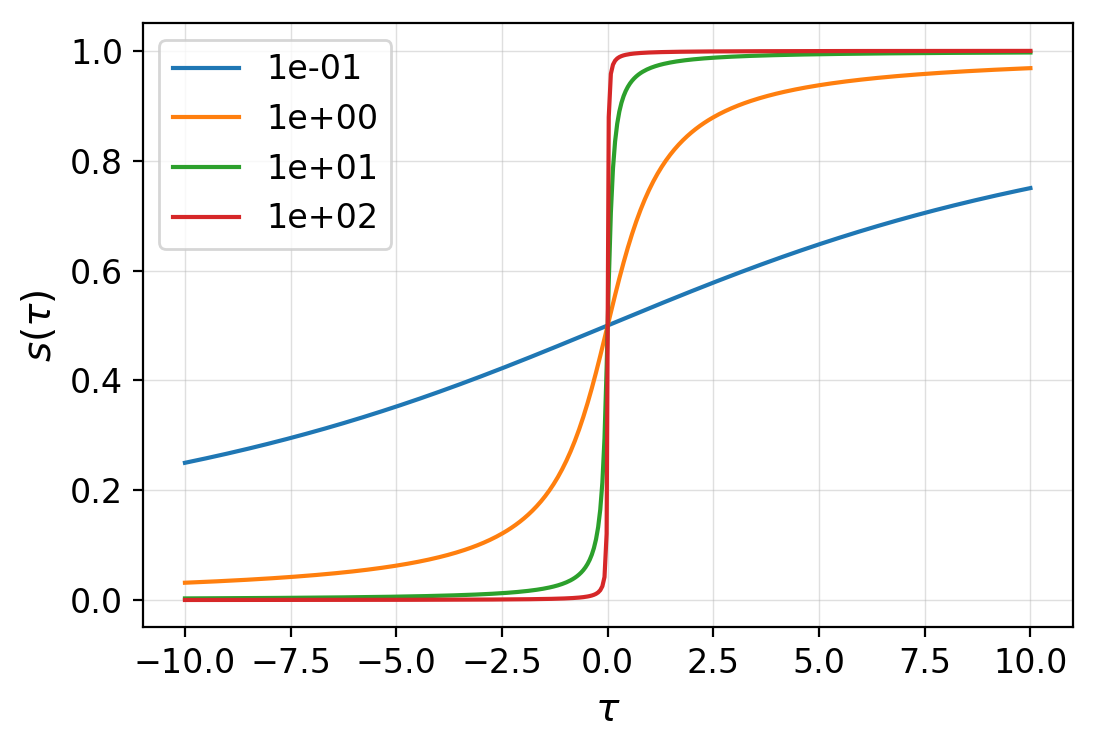
\includegraphics[width=0.6\textwidth]{figures/inversion/approx_step.png}
    \end{center}
\caption{
    Approximation to a step function using an arctangent, as described in equation
    \ref{eq:arctan_step}. The values in the legend indicate the value of the slope,
    $a$. Smaller values have a more gradual transition between zero and one, while
    larger values have a more rapid transition.
}
\label{fig:approx_step}
\end{figure}


To define a level set function for a block, I need to define a function, $\tau$, which evaluates to $\tau < 0$ when outside the target and $\tau > 0$ inside the target. To define a block, I could, for example use
\begin{equation}
\tau = 1 - \left(
    \left|\left|\frac{x - x_0}{\Delta x / 2}\right|\right|_\infty^2 +
    \left|\left|\frac{y - y_0}{\Delta y / 2}\right|\right|_\infty^2 +
    \left|\left|\frac{z - z_0}{\Delta z / 2}\right|\right|_\infty^2
\right)
\label{eq:tau_infinity}
\end{equation}

however, the infinity norm is not differentiable. Thus, I approximate the infinity norm using an Ekblom norm \citep{Ekblom1973},
\begin{equation}
\tau = 1 - \left(
    \left[\left(\frac{x - x_0}{\Delta x / 2}\right)^2 + \varepsilon^2 \right]^{p/2} +
    \left[\left(\frac{y - y_0}{\Delta y / 2}\right)^2 + \varepsilon^2 \right]^{p/2} +
    \left[\left(\frac{z - z_0}{\Delta z / 2}\right)^2 + \varepsilon^2 \right]^{p/2}
\right)
\label{eq:tau_ekblom}
\end{equation}

where $\varepsilon$ is a small constant and $p$ is a constant describing the approximate norm, for example, if $p=2$, then equation \ref{eq:tau_ekblom} describes an ellipsoid. To represent a block, I choose a $p$ that is sufficiently large. For the length scales I consider, a value of $p=4$ is appropriate. The value of $\varepsilon$ is chosen to be large enough, and the value of $p$ small enough so that the derivatives of the mapping are stable and second-order for the length scales of the problem. In addition, rotations can be included in the model, as described in \cite{Mcmillan2017} \footnote{\cite{Mcmillan2017} also employs a weighting scheme to scale the model parameters. I have not found this to be necessary for the examples I consider and thus do not use any weights or scaling}.

When employing parametric mappings, there are two important implications to note in the setup of the inversion. Since the mathematical statement of the inverse problem is, in principle, overdetermined (there are more data than model parameters), I fix the value of $\beta$ at zero and do not employ a regularization. The second point is that for a starting model, it is important to start with the block and background having different conductivities. This was similarly discussed in \cite{Mcmillan2017}.

\subsubsection{Effective medium theory mapping}
\label{sec:emt_mapping}

In Chapter \ref{ch:phys-prop-model}, I introduced a two-step process for estimating the electrical conductivity of a propped, fractured volume of rock. The first step involved estimating the effective conductivity of a mixture of electrically conductive proppant and fluid, and in the second step, I estimated the effective conductivity of a volume of rock which has fractures filled with the proppant-fluid composite.

Assuming the electrical conductivity of the fluid and proppant are known, then rather than inverting for electrical conductivity, we can invert for the concentration of conductive fractures. To avoid introducing additional non-uniqueness into the problem, I use a fixed ratio of proppant and fluid within the propped region of the reservoir and treat the fracture concentration $\varphi$ as the inversion model (e.g. $\mathbf{m} = \varphi$). In a voxel-based inversion, $\varphi$ is a vector with a value for the concentration in each cell. For simplicity, I assume that the fractures are randomly oriented and work only with isotropic conductivities. In this case, the mapping requires that we solve the two-pahse effective medium theory approximation,
\begin{equation}
    (1-\varphi)(\sigma^* - \sigma_0)R^{(0,*)} + \varphi(\sigma^* - \sigma_1)R^{(1,*)}= 0
\label{eq:effective_medium_theory_mapping}
\end{equation}

for the effective conductivity, $\sigma^*$. The background has conductivity $\sigma_0$ and the conductive, proppant-filled cracks have conductivity $\sigma_1$. Note that $\sigma_0$, the conductivity of the background, does not need to be a scalar, it can be a vector with a background conductivity value for each voxel in the mesh. These values can be obtained by first inverting the pre-fracture data. The electric field concentration tensor $R^{(i,*)}$ captures the geometry of the particles that compose each phase. Note that for randomly oriented fractures $R^{(i,*)}$ is a scalar ($1/3 \text{trace}{\mathbf{R}^{(i,*)}}$, where $\mathbf{R}^{(i,*)}$ is given in equation \ref{eq:emt_r_ellipsoids}:
\begin{equation}
    R^{(j,*)} = \frac{1}{3}\text{trace}\left(\left[\mathbf{I}+\mathbf{A}{\sigma^*}^{-1}(\sigma_j-\sigma^*)\right]^{-1}\right)
\label{eq:emt_r_ellipsoids_random}
\end{equation}

For the background, I use an aspect ratio of 1, assuming a spherical geometry for the particles that compose it, and for the fractures, I use a small aspect ratio ($\sim 10^{-4} - 10^{-3}$) and treat them as ellipsoidal cracks. In Section \ref{sec:emt-rock-volume}, I demonstrated that for sufficiently thin fractures, the exact aspect ratio is not significant. For a gradient based inversion, we also require the derivative of the effective conductivity, $\sigma^*$, with respect to our model, which is the fracture concentration, e.g.
\begin{equation}
    \frac{\partial \sigma}{\partial \mathbf{m}} = \frac{\partial\sigma^*}{\partial \varphi}
\label{eq:deriv_emt}
\end{equation}

 This derivation is outlined in Appendix \ref{app:scemt-derivs}.

The general time-lapse inversion workflow using effective medium theory is two steps:
\begin{itemize}
    \item{Construct a background conductivity model, $\sigma_0$, by inverting pre-fracture data. This inversion is a voxel-inversion for log-conductivity.}
    \item{Invert the post-fracture data for fracture concentration, $\phi$. Note that using a starting model and reference model of $\mathbf{m_0} = \mathbf{0}$ is equivalent to starting the post-fracture inversion with the pre-fracture model.}
\end{itemize}

Self-consistent effective medium theory is the method I adopt to connect the concentration of fractures with the effective conductivity of a fractured volume of rock, however, other relationships, such as an empirical relationship estimated from a lab study, could equally be employed. One interesting implication of relating the concentration of the fractures to the change in conductivity is that this provides a conduit for bringing in a-priori information about the volume of proppant injected into the reservoir. The predicted volume is
\begin{equation}
    V_{\rm pred} = \int\varphi ~ dV
\label{eq:predicted_volume}
\end{equation}

I can then define a volume data misfit term,
\begin{equation}
    \phi_V = \frac{1}{2}\left|\left|\frac{1}{\varepsilon_V}(V_{\rm pred} - V_{\rm obs})\right|\right|^2
\label{eq:volume_data_misfit}
\end{equation}

where $V_{\rm obs}$ is the known volume terms which accounts for the estimated ratio of proppant and fluid and $\varepsilon_V$ is an uncertainty term. I note that I am assuming a fixed ratio of proppant and fluid within the cracks. In reality, this will be variable, thus I use a sufficiently large $\varepsilon_V$ so as not to over-fit this assumption.

In the implementation, the inclusion of an additional data misfit term is handled by a combo-objective function which enables joint inversions in the SimPEG framework.

\section{Inversions with steel-cased wells}

In the Chapter \ref{ch:casing-dc}, we saw that the current spreads out along the length of the casing, decaying as we move away from the source. In the inversion, this raises questions about our ability to resolve the depth and vertical extent of the target. In this section, I start from a simple model of a vertical well with a conductive target and examine our ability to recover that target. Although most fracture operations are conducted in horizontal wells, I start by considering a vertical well as this reduces computational cost and allows us to explore aspects of the behavior of inversion prior to moving to the more fully 3D, more computationally intensive scenario.

I start by considering a DC experiment with a simple cylindrically symmetric model, shown in Figure \ref{fig:DC_cyl_setup}. A 1 km long casing is embedded in a background that has a resistivity of of $100$ $\Omega$m. The casing has an outer diameter of 10 cm, a thickness of 1 cm and a conductivity of $5 \times 10^6$ S/m. For modelling, I approximate the hollow-cased well as solid cylinder with a conductivity of $1.4 \times 10^4$ S/m, which preserves the product of the conductivity and the cross sectional area. This was shown to be a valid approximation for DC problems in Section \ref{sec:approximating_wells} and allows us to reduce the number of cells in the mesh, thus speeding up the computation of the forward simulation and sensitivities. Similar to the model used in \ref{ch:phys-prop-model}, I assume a moderately-sized fracture operation which uses an 800 m$^3$ slurry comprised of $15\%$ proppant by volume. I assume leak-off of some of the fluid, leaving a mixture of 50\% fluid and 50\% proppant, by volume, in the fractures. This gives a total fracture volume of 240 m$^3$ which I distribute among 10 circular fractures. Each fracture is 3 mm wide is positioned within a 10 m interval along the well. Conserving volume gives a 50 m radius for the fractures. Using a fluid conductivity of 3 S/m and a proppant conductivity of 10$^5$ S/m, the conductivity of the 50/50 proppant-fluid mixture found using self-consistent effective medium theory (equation \ref{eq:effective_medium_theory}) is 2500 S/m. Using a fracture aspect ratio of $3 \times 10^{-5}$ and assuming randomly-oriented fractures, I obtain a conductivity of 3 S/m for the propped region of the reservoir.


\begin{figure}
    \begin{center}
    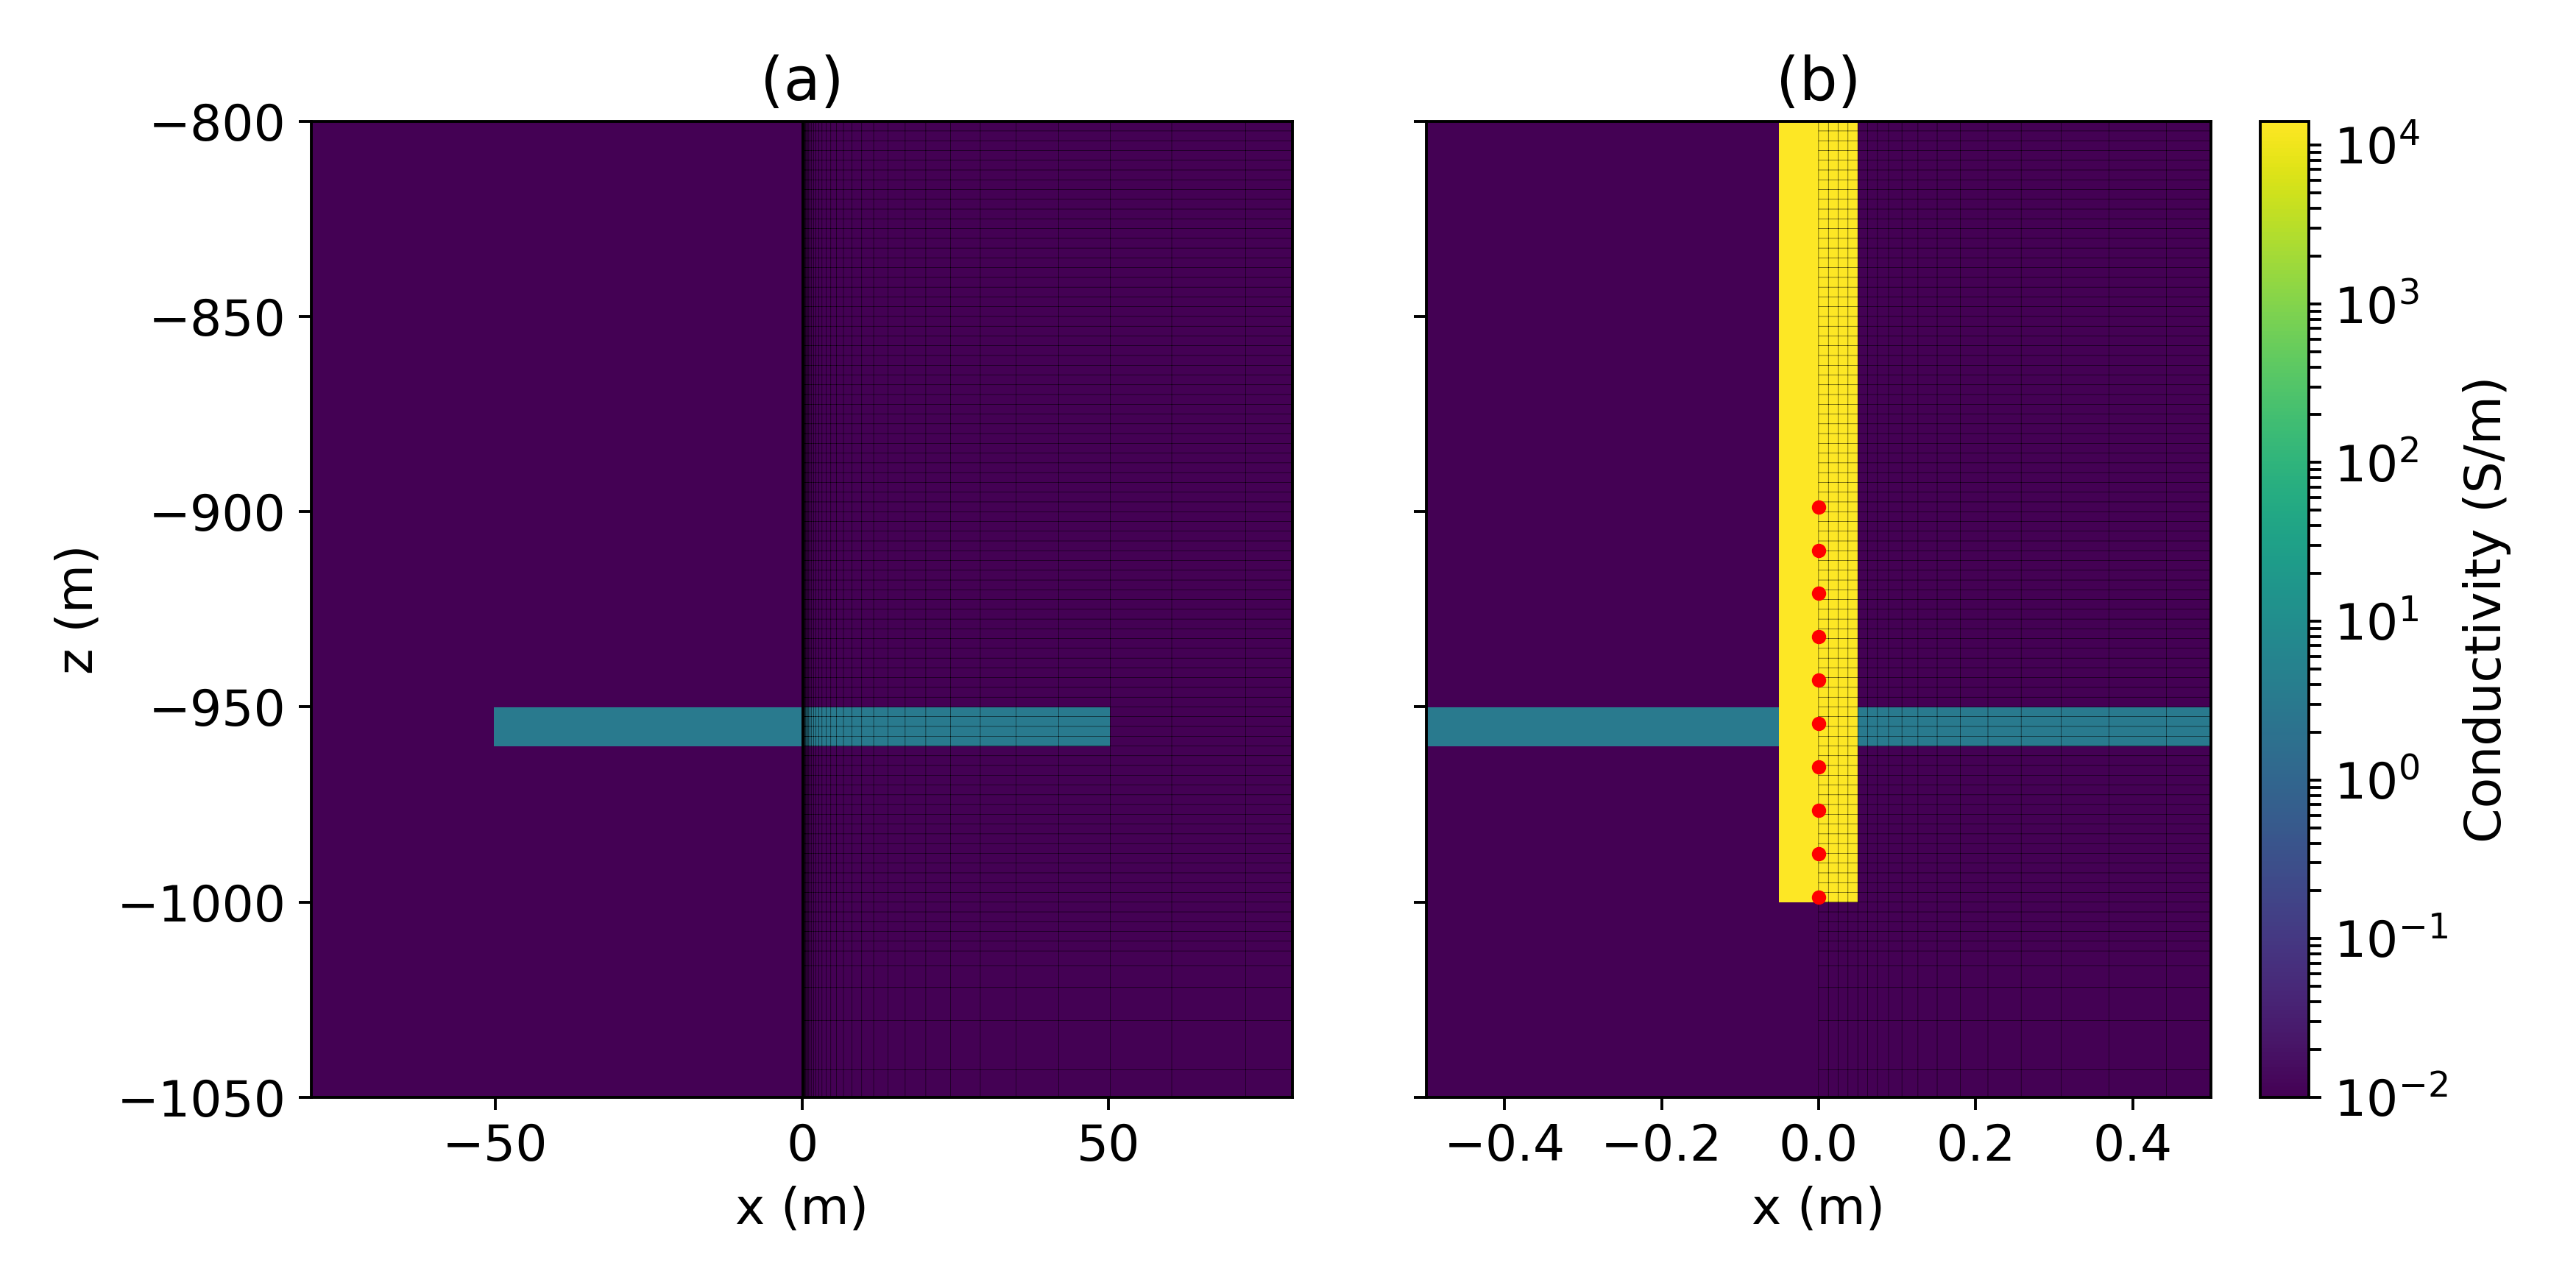
\includegraphics[width=\textwidth]{figures/inversion/DC_cyl_setup.png}
    \end{center}
\caption{
    Model of an electrically conductive propped fracture zone (3 S/m) in a halfspace (100 $\Omega$ m) with a steel-cased well.
    The well is modelled as a solid cylinder with a conductivity of $1.4 \times 10^4$ S/m. The mesh has 4 cells across the
    radius of the casing. The fractured region extends vertically from 950 to 960 m depth and has a radius of 50m.
    Panel (a) has a radial extent of 80 m to show the fractured zone and panel (b) has a radius of 0.4m to show the casing.
    The a-electrode locations are shown in panel (b).
}
\label{fig:DC_cyl_setup}
\end{figure}


The survey I use employs a downhole electrode and a distant return electrode. There are 10 down-hole source locations from 900 m depth to 1000 m depth, as shown by the red dots in Figure \ref{fig:DC_cyl_setup}b. Radial electric field data are collected at the surface; there are 40 receiver locations from 25 m to 1000 m along a radial line extending from the well. In total, the survey consists of 400 data. Figure \ref{fig:dc_casing_initial_data} shows (a) the simulated data for both the background (prior to the fracture) and the fracture, (b) the difference between the data with and without the fracture, and (c) the difference as a percentage of the background response. The color of each line indicates the depth of the positive electrode, as indicated by the colorbar at the bottom of the plot.The difference between the data simulated over is significant both in magnitude and in percentage and thus we can expect that the inversion will introduce structure in order to fit the fracture data. In the following sections, I will explore several approaches to the inverse problem for obtaining meaningful information from the data.


\begin{figure}
    \begin{center}
    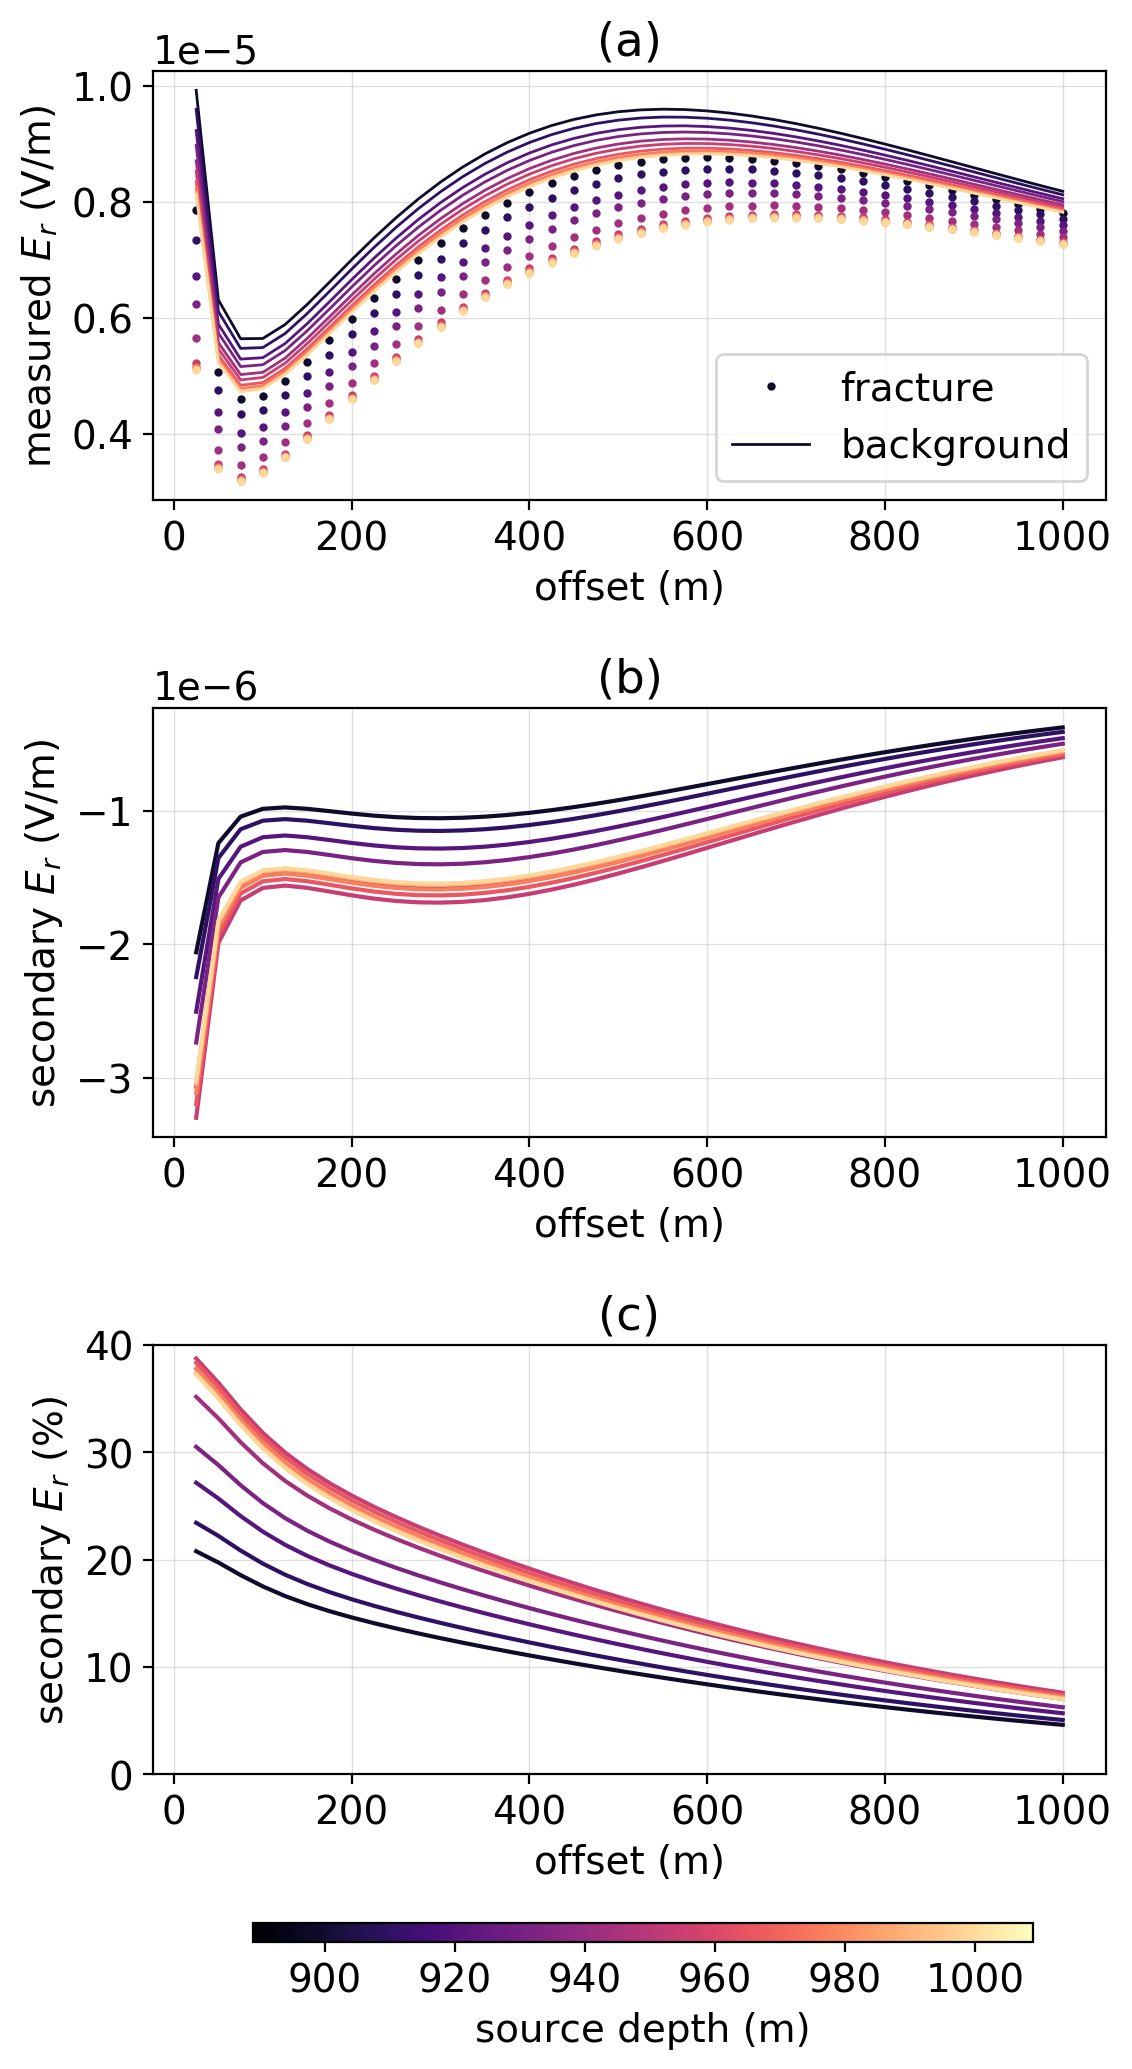
\includegraphics[width=0.6\textwidth]{figures/inversion/dc_casing_initial_data.png}
    \end{center}
\caption{
    (a) Synthetic data for the down-hole casing experiment for the background,
    prior to the fracture (solid lines), and after the fracture (dots), (b) secondary
    electric field (fracture - background), and (c) secondary electric field as a percentage
    of the primary (background). The color of the lines or dots indicates the depth of the source.
}
\label{fig:dc_casing_initial_data}
\end{figure}


\subsection{Voxel inversion for conductivity}
\label{sec:voxel_inversion}

I begin by applying standard inversion techniques and perform a voxel inversion using a Tikhonov regularization. As the simulation is cylindrically symmetric, I invert for a 2D model which varies radially and vertically. Our aim in this inversion and the ones that follow is to examine, under ideal circumstances, what information we can obtain from the data using a given inversion approach. I therefore do not add noise to the data and assign low uncertainties: 1\% with a $10^-9$ V/m floor.

The choice of parameters is quite standard, similar to how one would approach a blind inversion. In the regularization, I use $\alpha_s = 10^{-3}$, $\alpha_x = \alpha_z = 1$. I start the inversion with a large value of $\beta$, so that the regularization term initially dominates the objective function, and reduce the its value over the course of the inversion. The initial and reference model are equal to the half-space resistivity of 100 $\Omega$m.

The results of the first inversion I run are shown in Figure \ref{fig:dc_smooth_inversion_1e-01}. This inversion reached a global $\chi$-factor of $<0.1$ and fits all data points within 5\% (Figure \ref{fig:dc_smooth_inversion_1e-01}c). It converged in two iterations.  Because of the regularization function being used, the recovered model is smooth and diffuse. Perhaps unexpected is the location of the center of the recovered target; its depth is shifted below the true location, closer to the end of the well. Typically, we might expect that if the inversion were to shift the location of a target, it would be shifted up, closer to the receivers, where we have greater sensitivity. However, the presence of the casing alters the sensitivity. In Chapter \ref{ch:casing-software}, I demonstrated that there is an increase in charge near the ends of the well (see Figure \ref{fig:kaufman_finite_well}, in particular), for the DC problem, this translates to an increase in sensitivity near the end of the well. This can also be seen by plotting the sensitivity. In Figure \ref{fig:casing_sensitivity}, I plot the sensitivity function for the starting model of the casing in a 100 $\Omega$m half-space (a) and (b), as well as for the true model, with the conductive target in (c) and (d). In panels (a) and (b), we see that throughout the region where the source electrodes are positioned, the sensitivity is relatively uniform. The exception is near the end of the well, where the region of large sensitivity broadens. When the target is included, the sensitivity is increased in that region. However, we still see a broadened region of high sensitivity near the bottom of the well. The increase in high sensitivity near the end of the well has a tendency to promote structure near the end of the well in the inversion.


\begin{figure}
    \begin{center}
    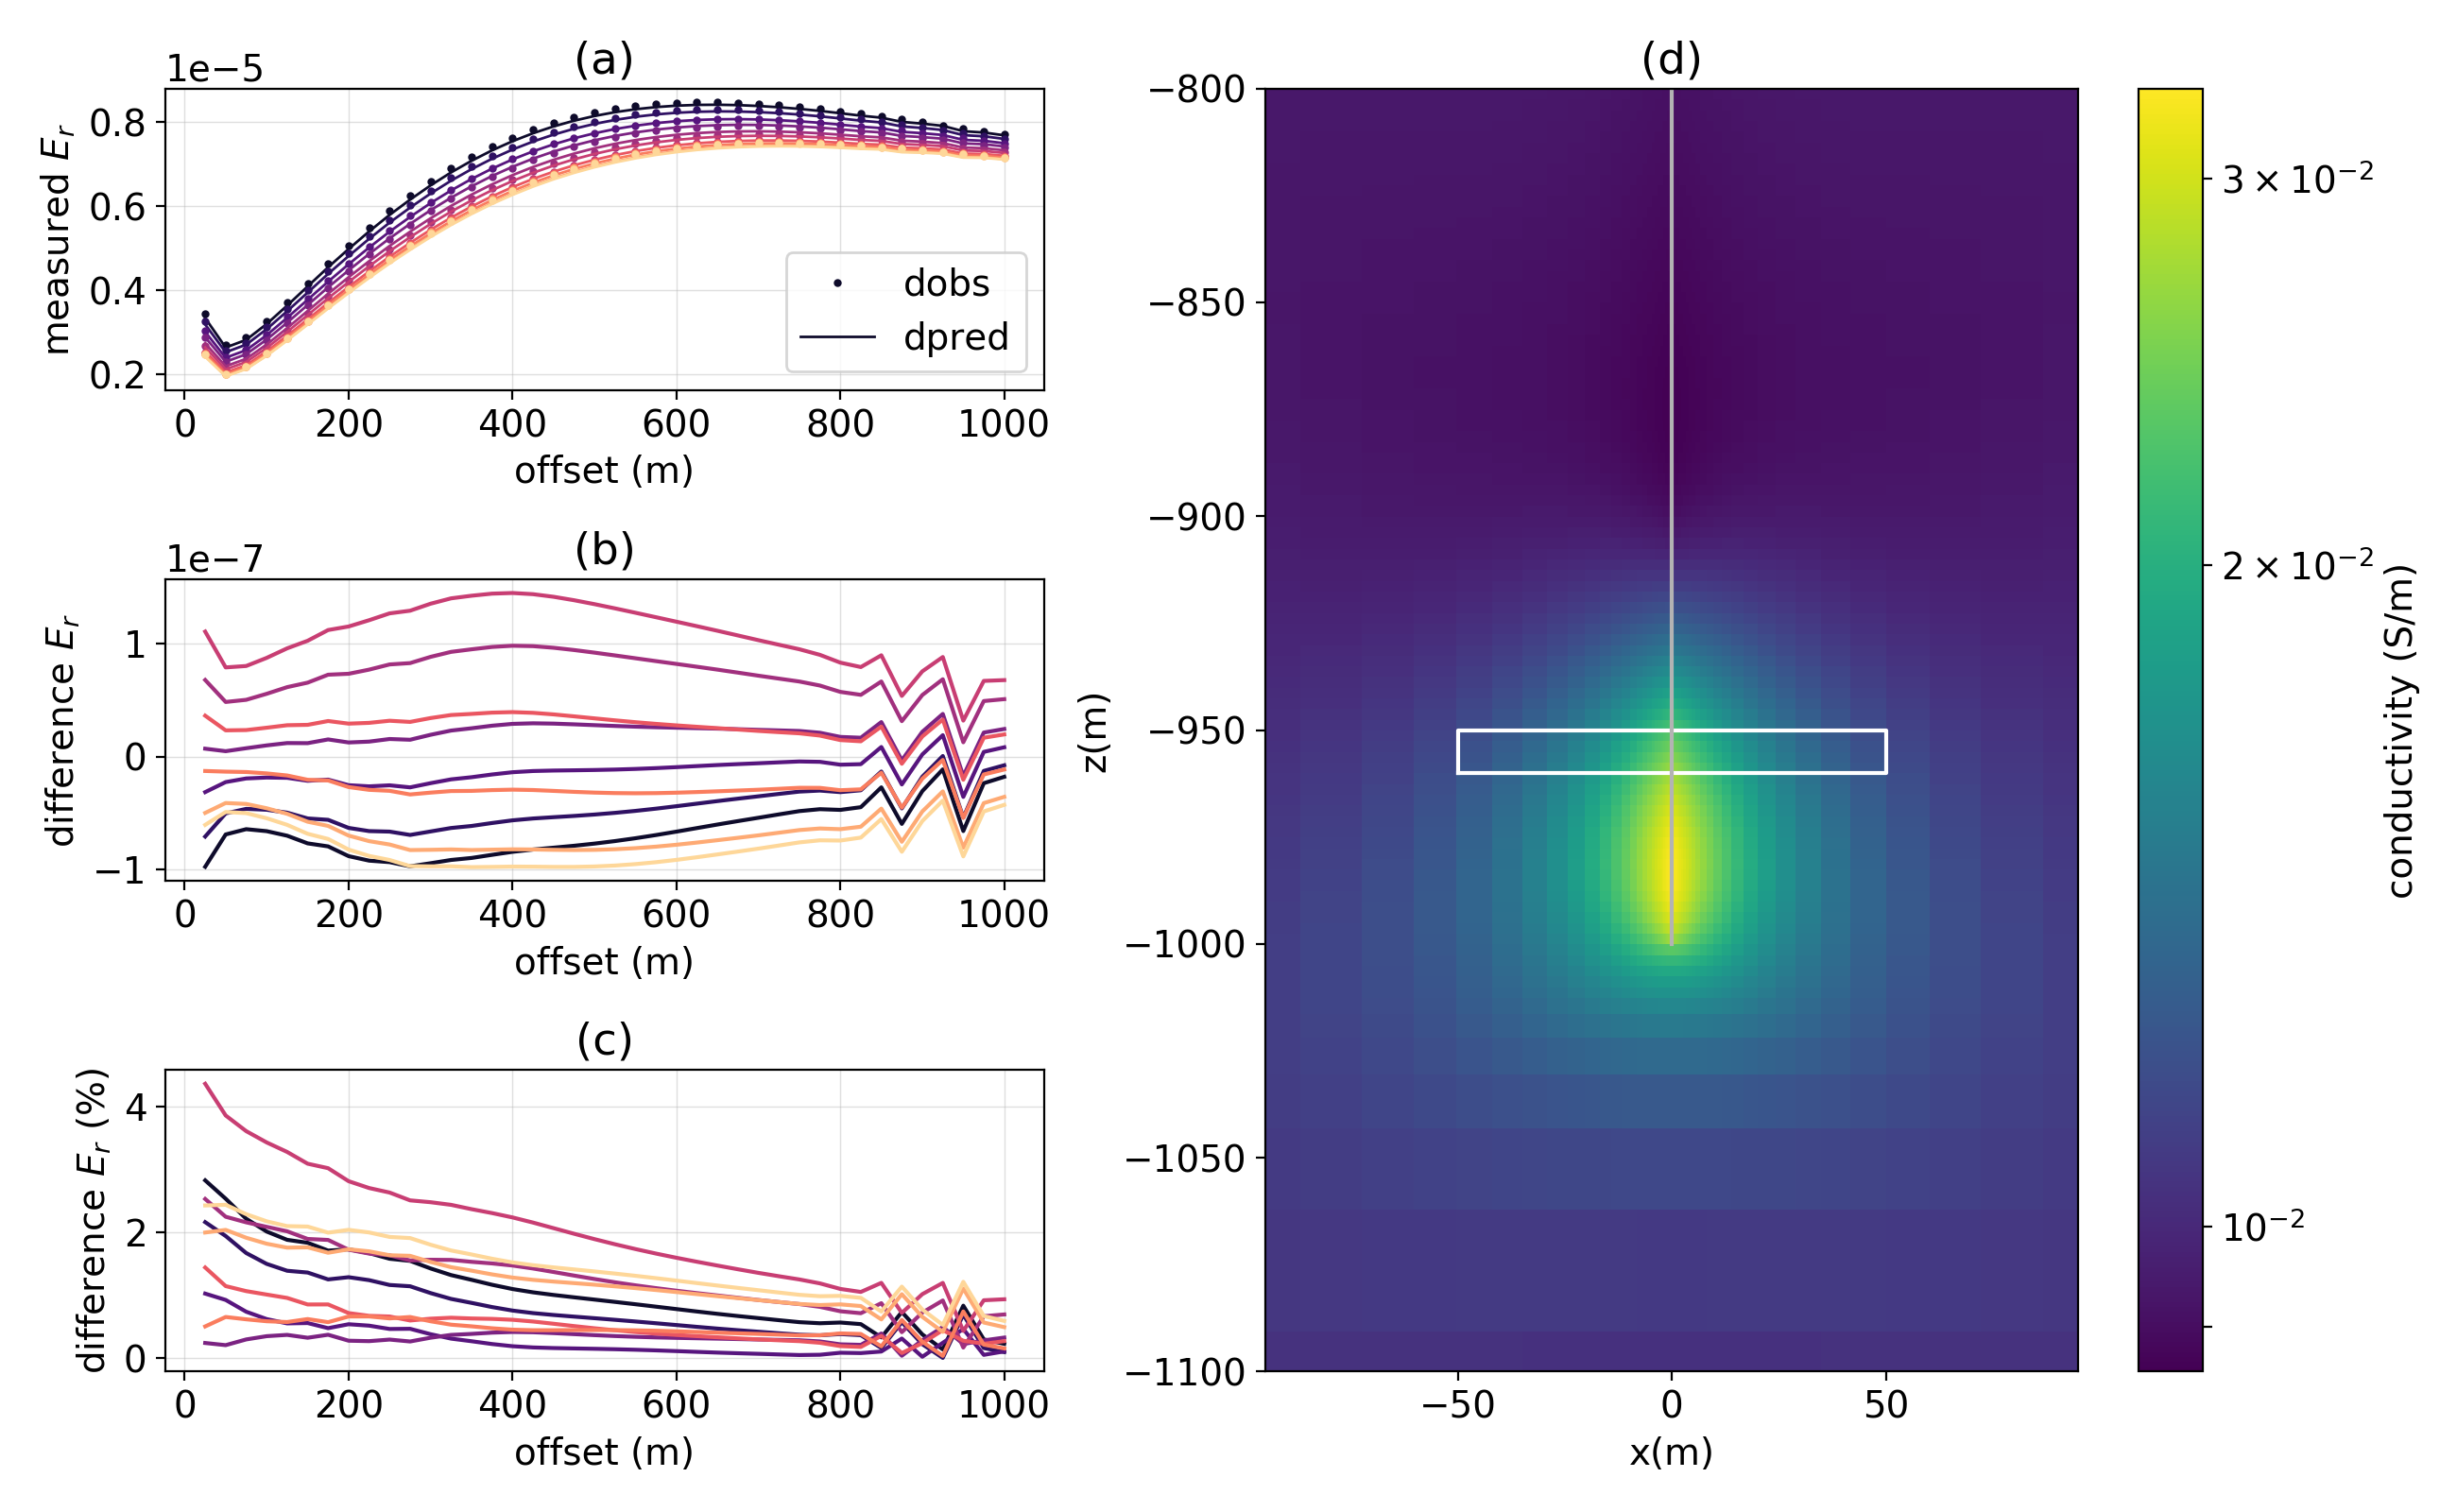
\includegraphics[width=1\textwidth]{figures/inversion/dc_smooth_inversion_1e-01.png}
    \end{center}
\caption{
    (a) Observed and predicted radial electric field data,
    (b) difference between the observed and predicted data (V/m),
    (c) difference between the observed and predicted data as a percentage of the observed data,
    and (d) conductivity model recovered in the inversion.
    The colors in (a), (b), and (c) indicate the source location as shown in Figure \ref{fig:dc_casing_initial_data}.
    The white outline in (d) outlines the true geometry of the fracture zone and the grey line shows the location of the wellbore.
    The data are fit to a global $\chi$-factor $<$ 0.1.
}
\label{fig:dc_smooth_inversion_1e-01}
\end{figure}





\begin{figure}
    \begin{center}
    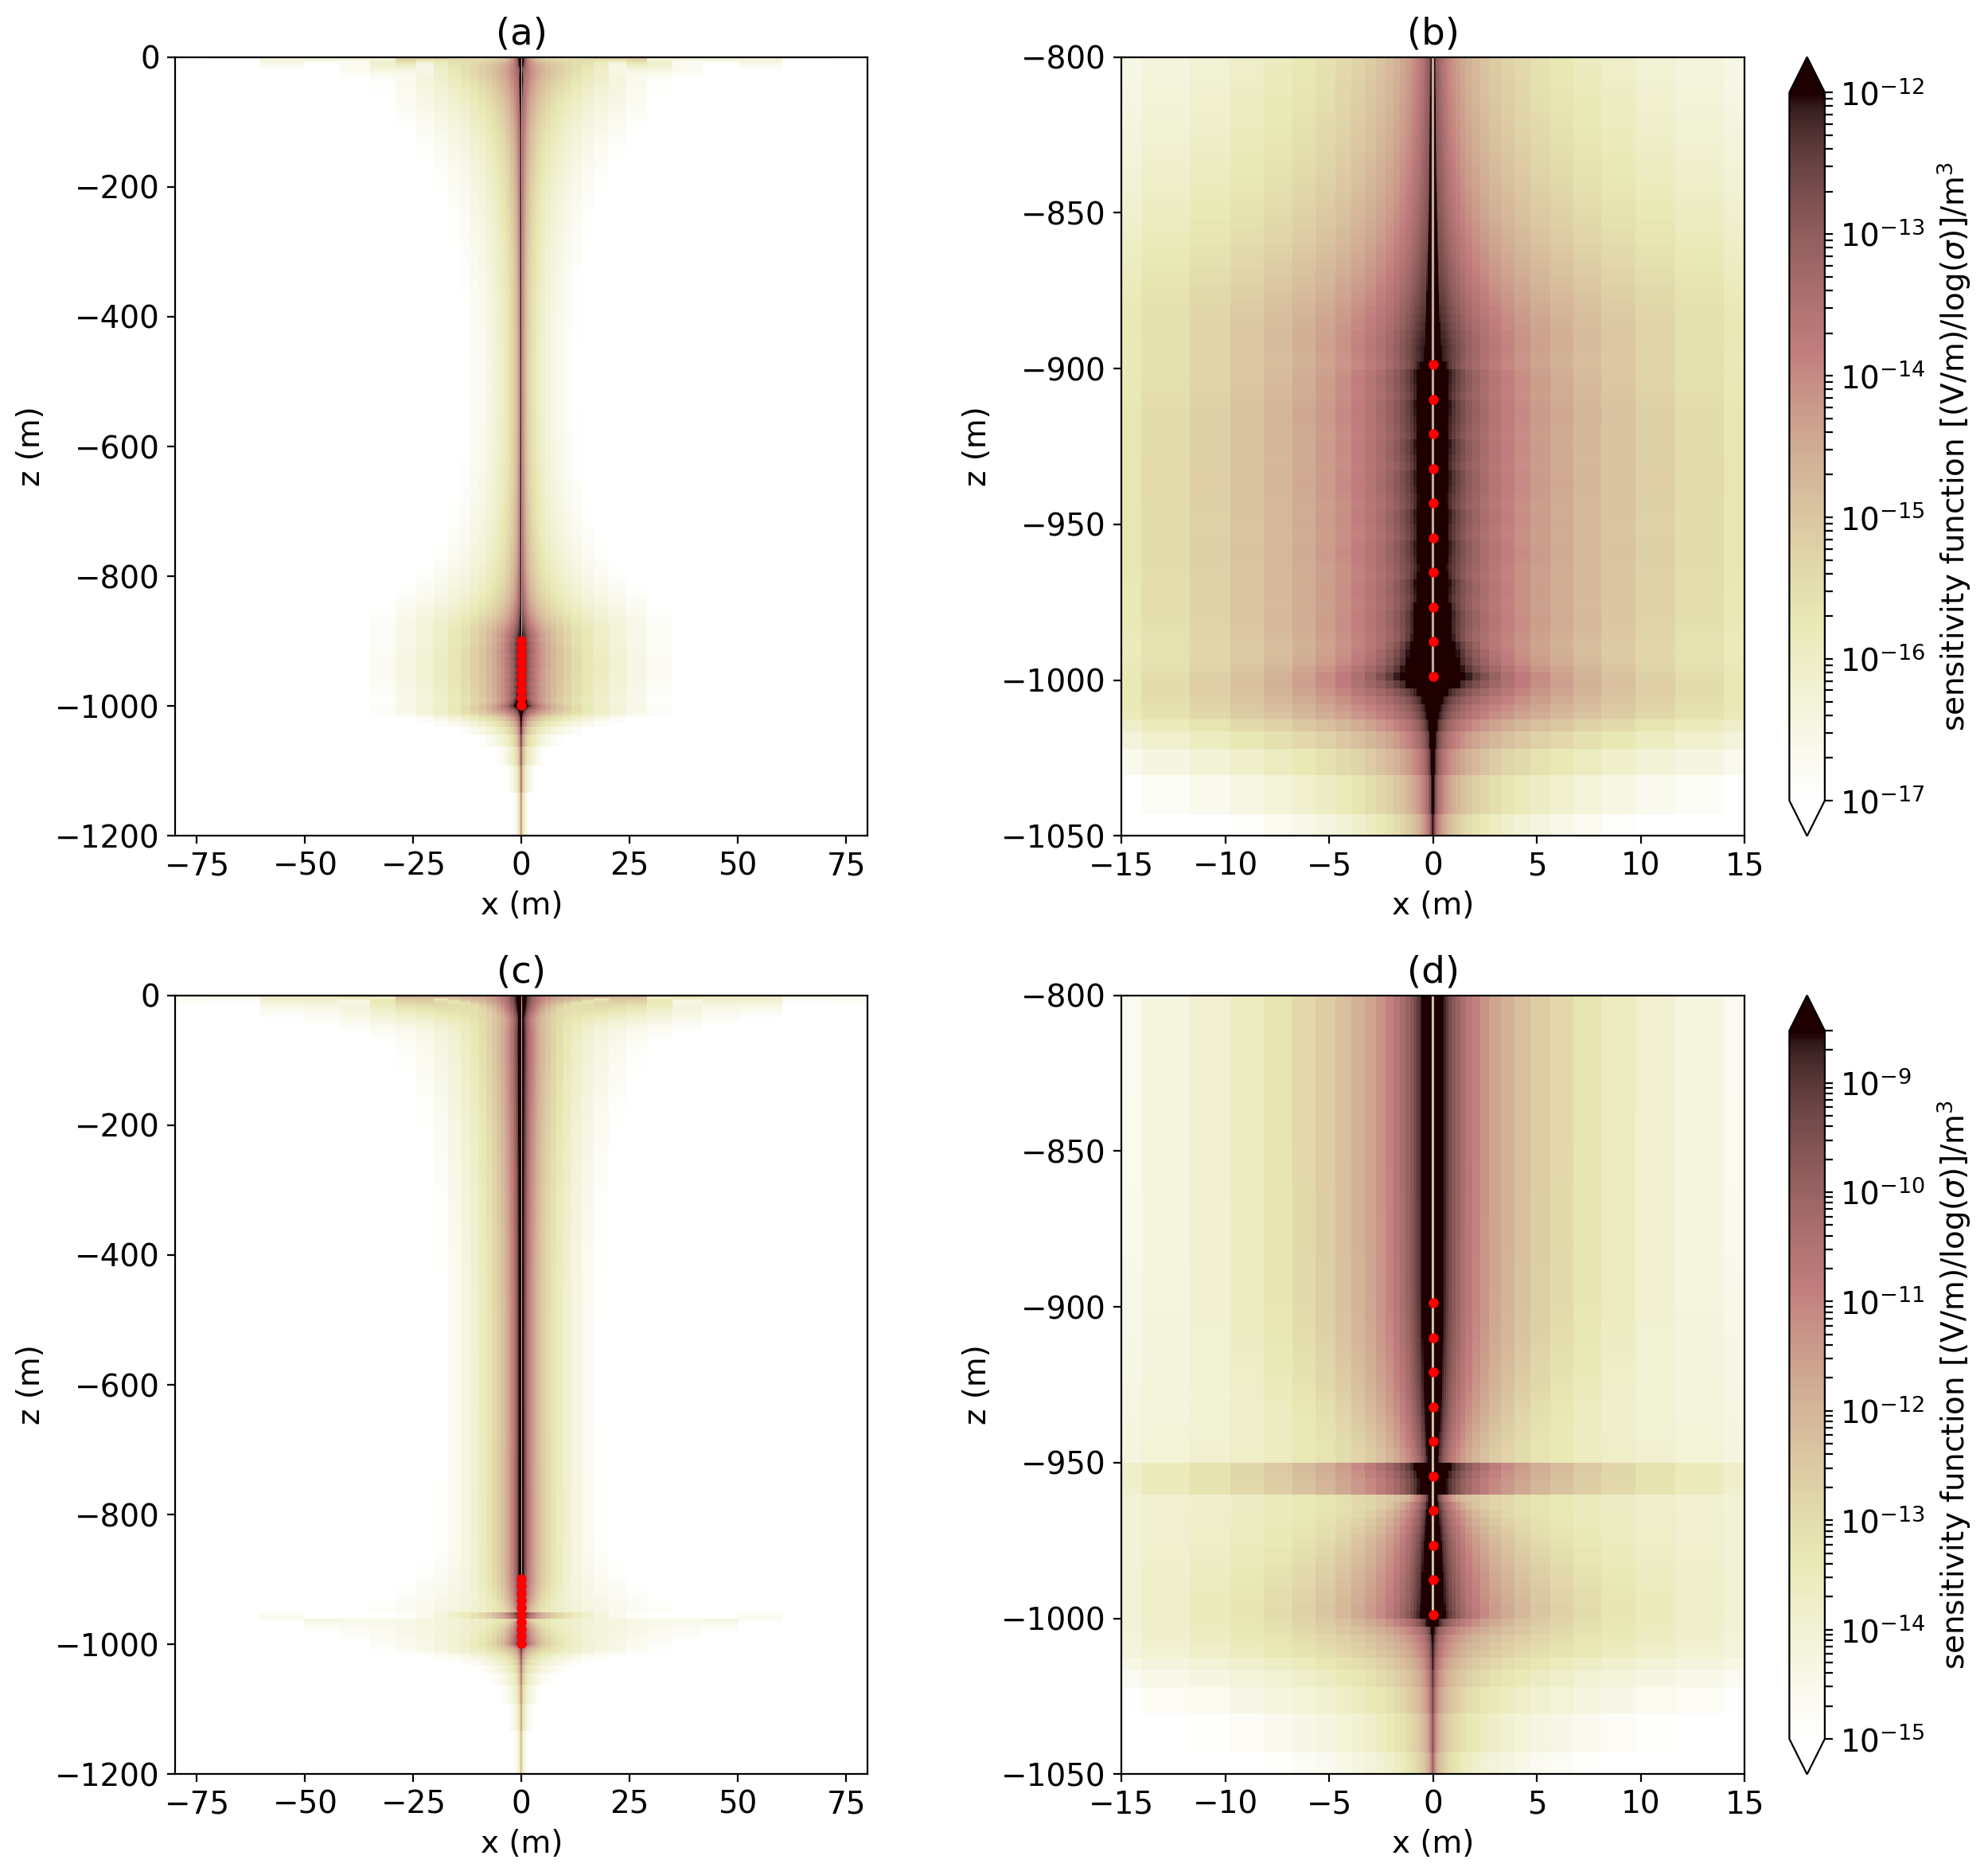
\includegraphics[width=\textwidth]{figures/inversion/casing_sensitivity.png}
    \end{center}
\caption{
    Integrated sensitivity for (a, b) a survey conducted in a 100 $\Omega$m half-space and
    (c, d) the true model with the conductive target, shown in Figure \ref{fig:DC_cyl_setup}.
    The inversion model is log-conductivity.
    The casing is
    shown by the grey line, and the source locations are shown by the red dots. The integrated sensitivity
    is computed by squaring the elements of the sensitivity matrix, summing along the rows of the sensitivity
    matrix and then taking the square-root. This gives a vector whose length is the number of model parameters.
}
\label{fig:casing_sensitivity}
\end{figure}


If I push the inversion harder and try to further improve the data-fit, the depth of the target is better-resolved, as shown in Figure \ref{fig:dc_smooth_inversion_5e-02}. In practice, this requires very high data quality; here I fit all data points within $\sim2\%$ and reach a global $\chi$-factor $<$0.05. The geometry of the target that I recover is elongated vertically; this is consistent with having larger sensitivity near the well. We also notice that the conductivity of the region above the target drops beneath that of the background -- this is a common effect in smooth inversions when conductive targets are present. In this case, we know that the changes due to the conductive proppant and fluid should only increase the conductivity with respect to the background. I could impose a lower-bound on the conductivity of the inversion model, however, experimentation shows that this tends to push the center of the conductive anomaly beneath the true target depth.


\begin{figure}
    \begin{center}
    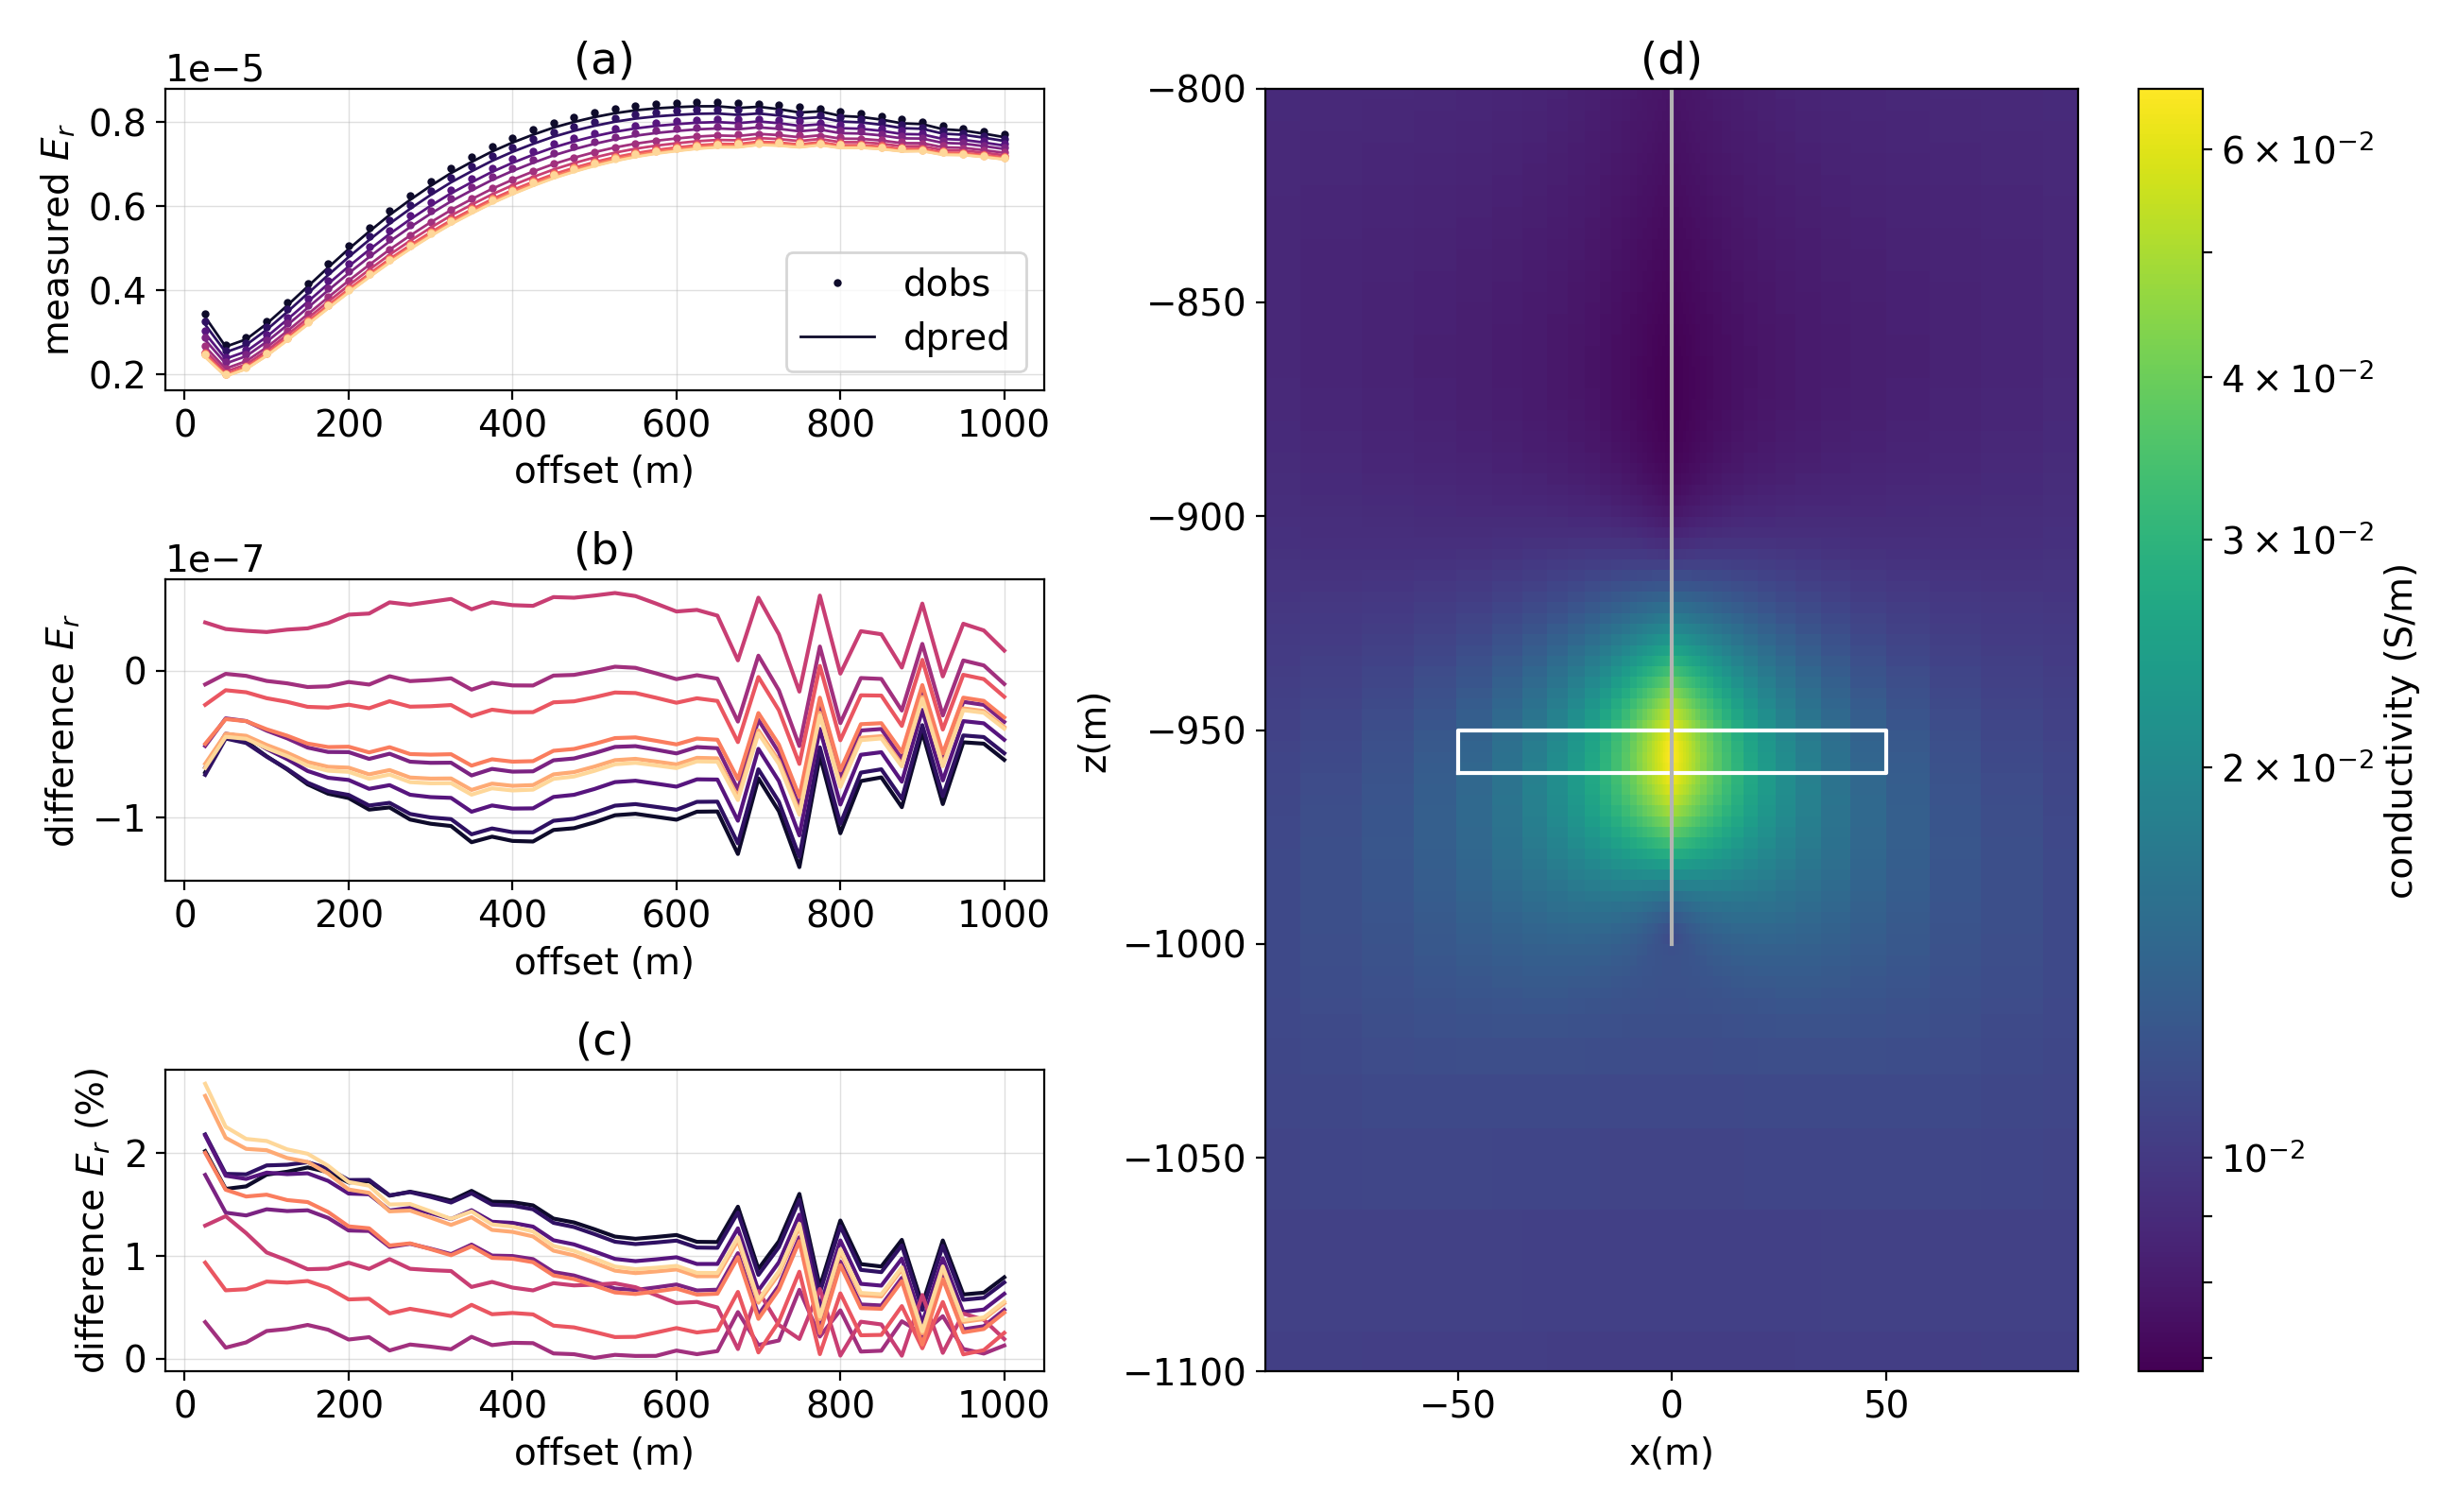
\includegraphics[width=1\textwidth]{figures/inversion/dc_smooth_inversion_5e-02.png}
    \end{center}
\caption{
    Tikhonov inversion result, similar to that shown in \ref{fig:dc_smooth_inversion_1e-01}
    that fits the data to a global $\chi$-factor $<$ 0.05.
}
\label{fig:dc_smooth_inversion_5e-02}
\end{figure}


More horizontally elongated structure can be promoted by altering the regularization. Figure \ref{fig:dc_smooth_inversion_5e-02_alpha_100} demonstrates an inversion using $\alpha_x=100$ and fitting the data to a $\chi$-factor $<$ 0.05. Using a large $\alpha_x$ smears out the target horizontally and also reduces the maximum conductivity as compared to Figure \ref{fig:dc_smooth_inversion_5e-02}.


\begin{figure}
    \begin{center}
    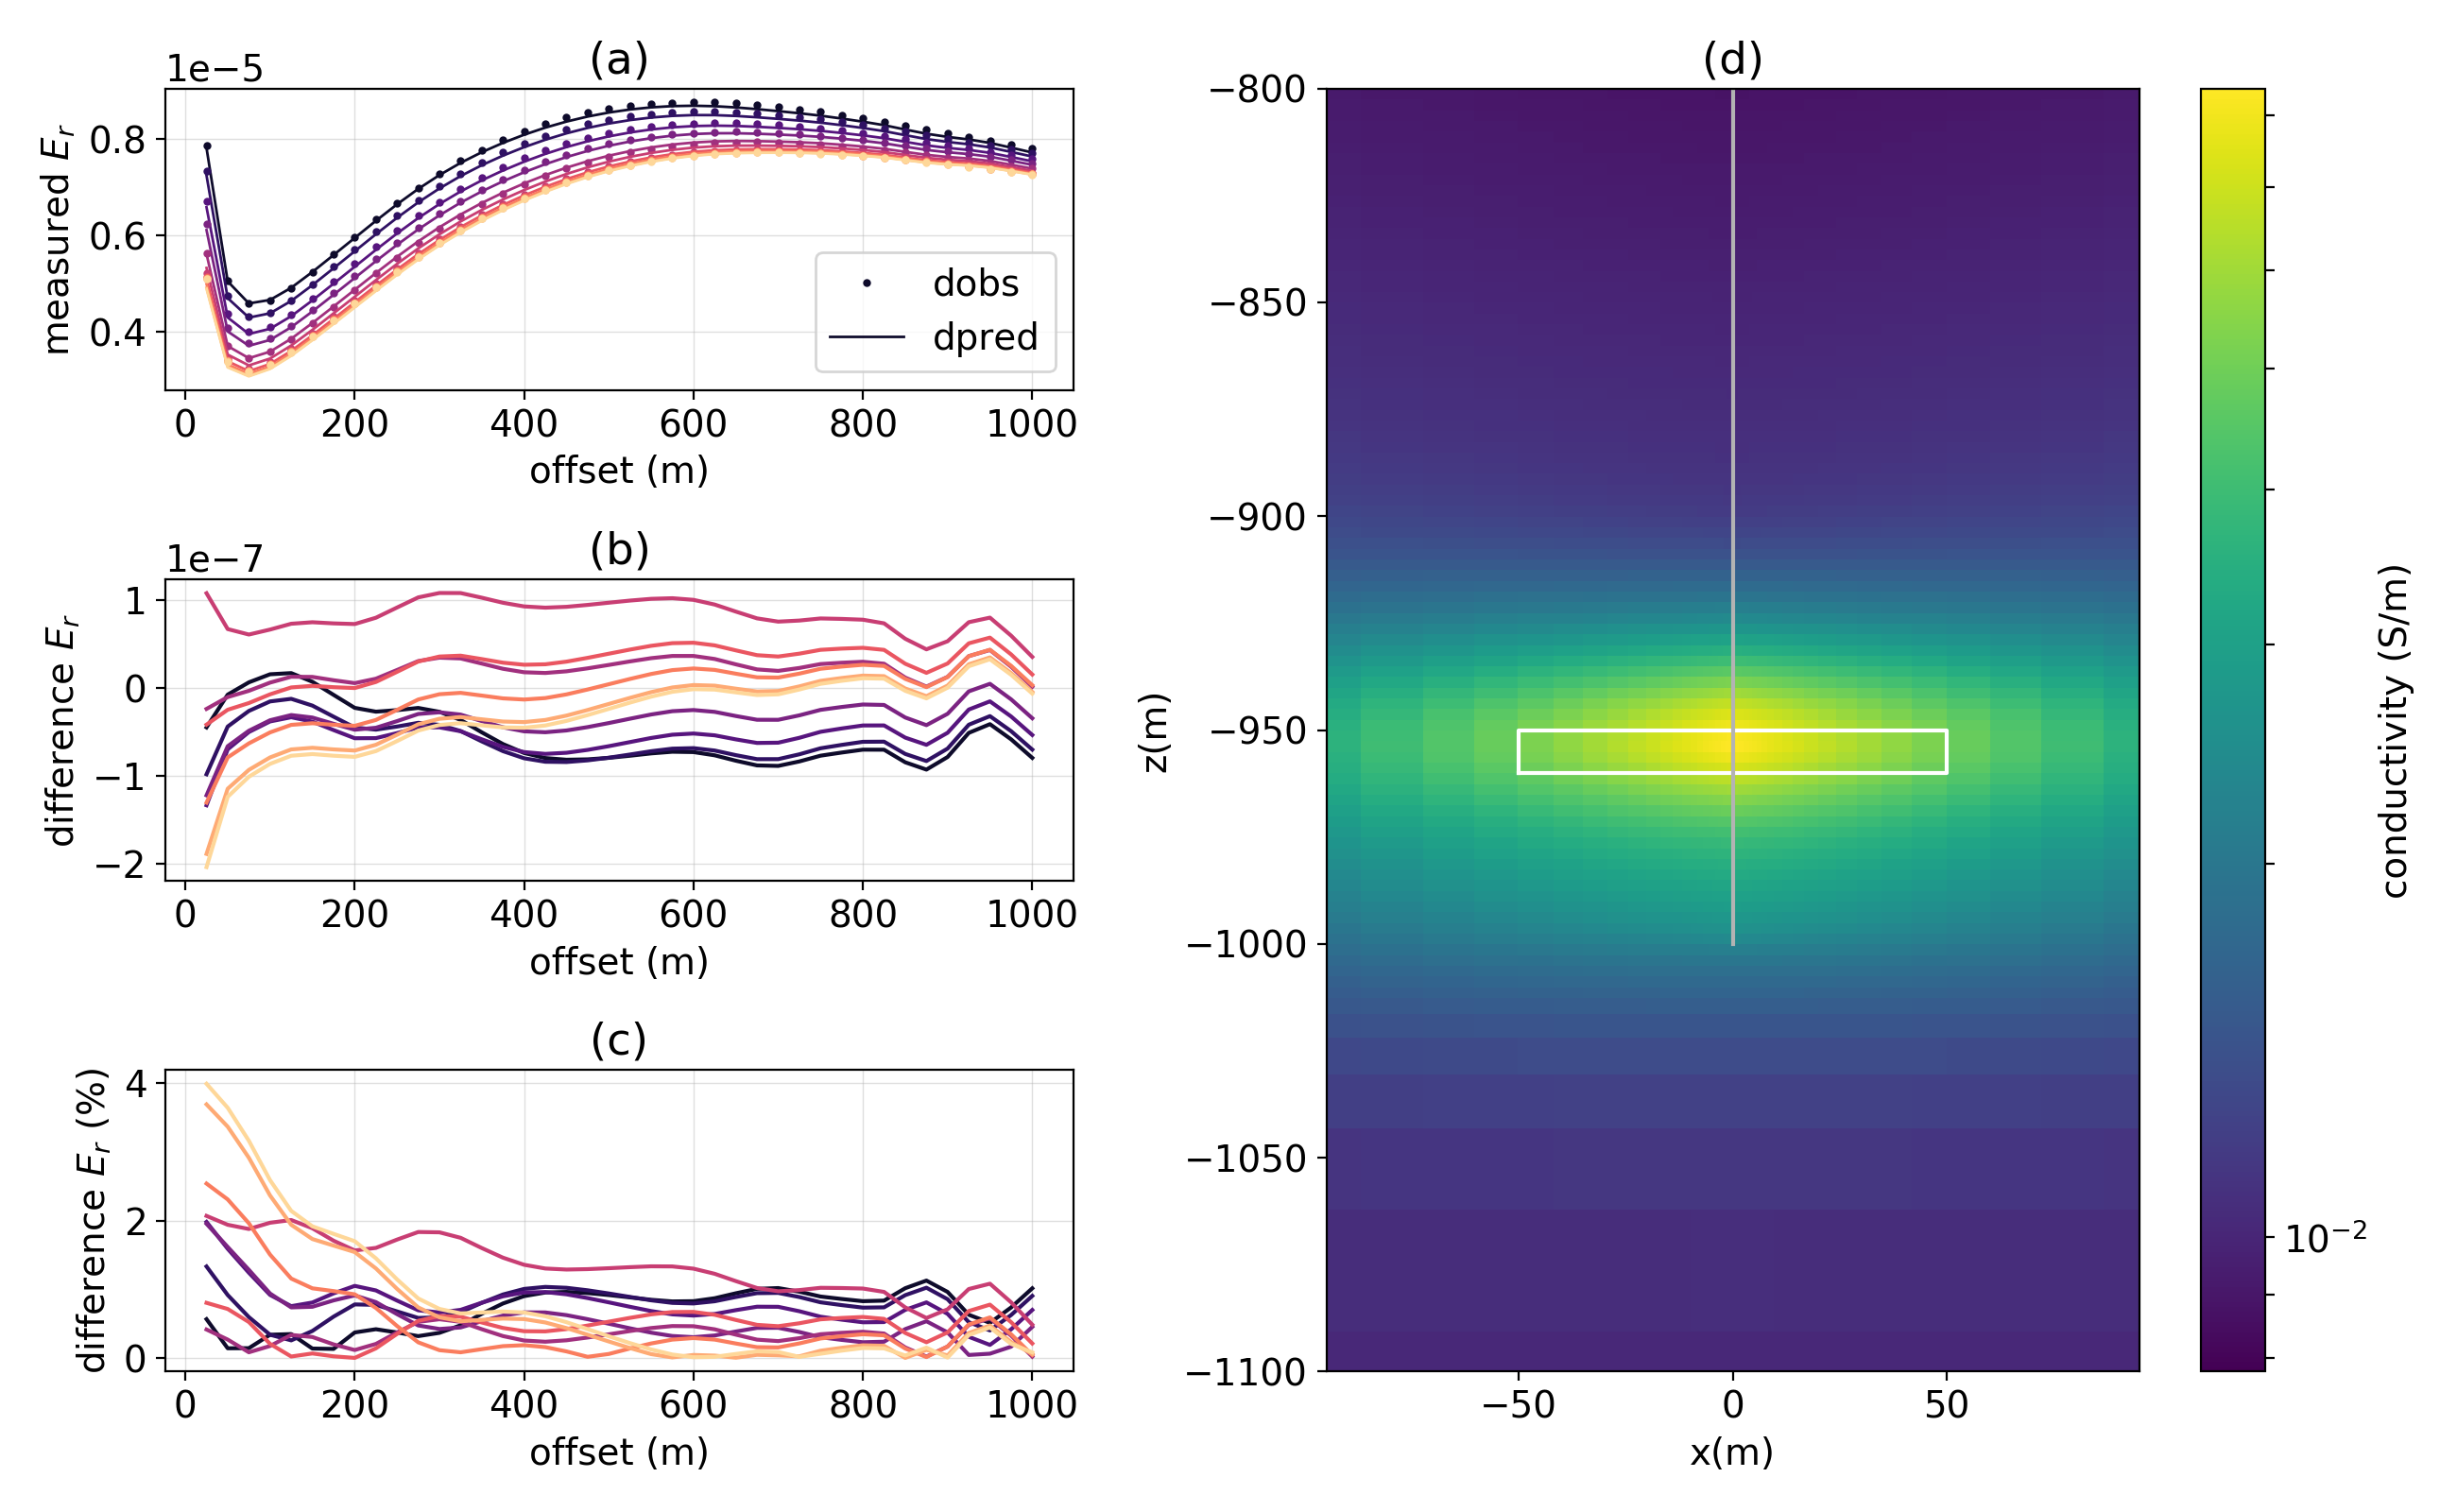
\includegraphics[width=0.8\textwidth]{figures/inversion/dc_smooth_inversion_5e-02_alpha_100.png}
    \end{center}
\caption{
    Tikhonov inversion result, similar to that shown in \ref{fig:dc_smooth_inversion_5e-02}
    that uses $\alpha_x = 100$. The inversion took 5 iterations.
}
\label{fig:dc_smooth_inversion_5e-02_alpha_100}
\end{figure}


In summary, by using a standard voxel inversion, we can recover a target at the correct location, and by adapting the $\alpha$ values, we can recover a general geometry reflective of the true target. However, these are not particularly insightful images for delineating the extent of the fractured region of the reservoir. With the aim of using the inversion to obtain parameters indicative of the injection, I next examine an approach using a parametric inversion.
\subsection{Parametric Inversion}
In a parametric approach to the inversion, the fractured volume of rock is represented as a simple geometric structure, and we invert for a handful of parameters that describe the properties of the background, target and the position and geometry of the target. For the following examples, I treat the fractured volume of rock as a cylinder. I fix $x_0 = 0$m and invert for the log-conductivity of the background and the target, as well as the depth, radius and thickness of the target. I again push the inversion quite hard, fitting the following results to a global $\chi$-factor $<0.05$, meaning that most of the data are fit within $\sim 2\%$.

For the parametric inversion to find an initial step, it is important that we start with a model where the target has physical properties distinct from the background. In this example, I build a starting model based on the first voxel inversion result, shown in Figure \ref{fig:dc_smooth_inversion_1e-01}. The center of the target is at 980 m depth, its radius is 5 m and it thickness is 5 m. The conductivity of the background is $10^{-2}$ S/m and the conductivity of the target is set to $3 \times 10^{-2}$ S/m. Figure \ref{fig:parametric_voxel1} shows the recovered model; the true geometry is outlined by the solid white line and the starting model geometry is shown by the dashed white line. The radius is underestimated (25 m) and the conductivity significantly overestimated ($7 \times 10^6$ S/m).


\begin{figure}
    \begin{center}
    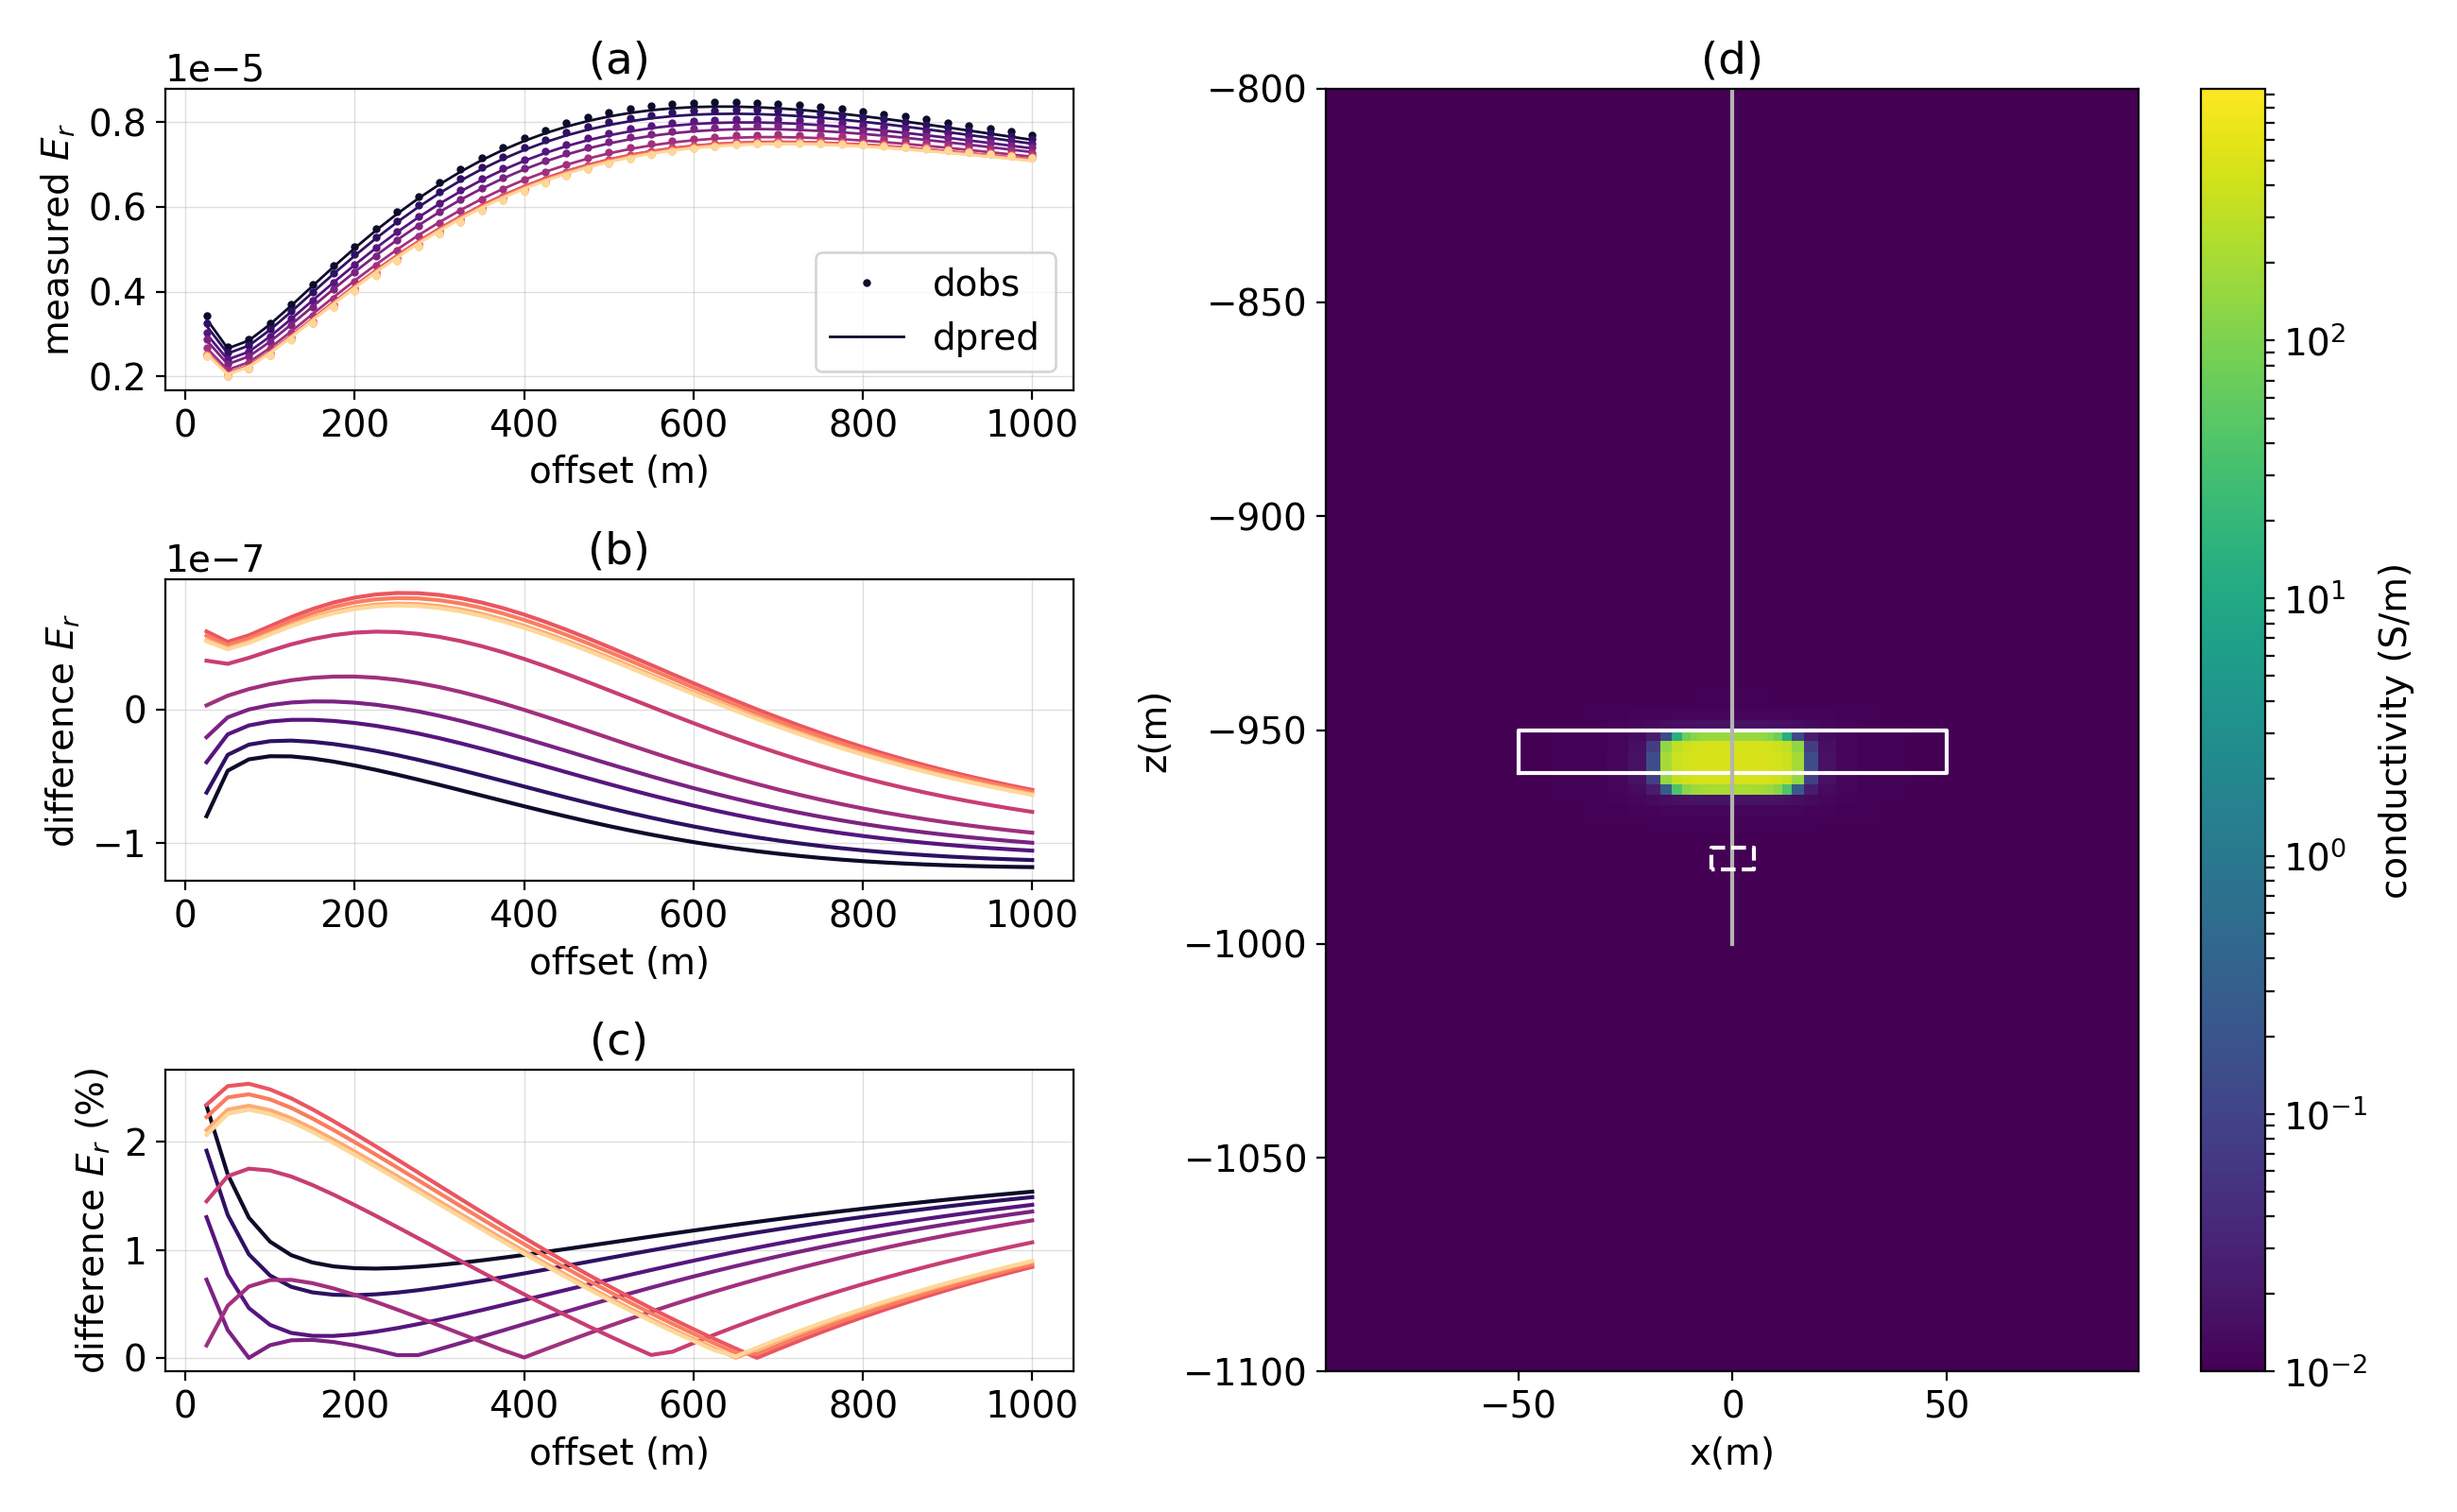
\includegraphics[width=1\textwidth]{figures/inversion/parametric_voxel1.png}
    \end{center}
\caption{
    Parametric inversion result for a starting model
    centered at 980m depth with a thickness of 5m and a radius of 10m. The initial background
    conductivity is $10^{-2}$ S/m and the initial conductivity of the target is $3\times10^{-2}$ S/m.
    The geometry of the starting model is shown by the white dashed-lines and the
    true model is shown by the solid white outline. The inversion reached a $\chi$-factor < 0.05
    and took 8 iterations.
\label{fig:parametric_voxel1}
\end{figure}


If instead, I use the true depth-center of the target, informed by the inversion result in Figure \ref{fig:dc_smooth_inversion_5e-02}, I obtain the model shown in Figure \ref{fig:parametric_voxel2}. The starting conductivities, radius and thickness were the same used in the previous inversion. In this inversion, the target is still shifted beneath the true location. The thickness, 12 m, is much closer to the true thickness (10 m). However, the recovered conductivity, $10^{10}$ S/m is even more severely overestimated than the previous inversion. Typically, one might expect that there is a saturation in the conductivity effects for a DC experiment. For example, if I consider the solution for a conductive sphere in a half-space subject to a uniform inducing electric field, the conductivity-dependence of the magnitude of the electric field external to the sphere is through the term:$(\sigma_2 - \sigma_1)/(\sigma_2 - 2\sigma_1)$, where $\sigma_2$ is the conductivity of the sphere and $\sigma_1$ is the conductivity of the background (see equation 6.67 in \cite{Ward1988}). For a fixed background conductivity, whether the conductivity of the target is 2 or 3 orders of magnitude larger than the background, makes little difference in the external electric field. However, in this example, the conductive target is directly coupled to the casing, which has a conductivity of $10^4$ S/m. I suspect that this survey geometry is sensitive to a larger dynamic range of conductivity values and this might contribute to the large updates in the electrical conductivity of the target.

\begin{figure}
    \begin{center}
    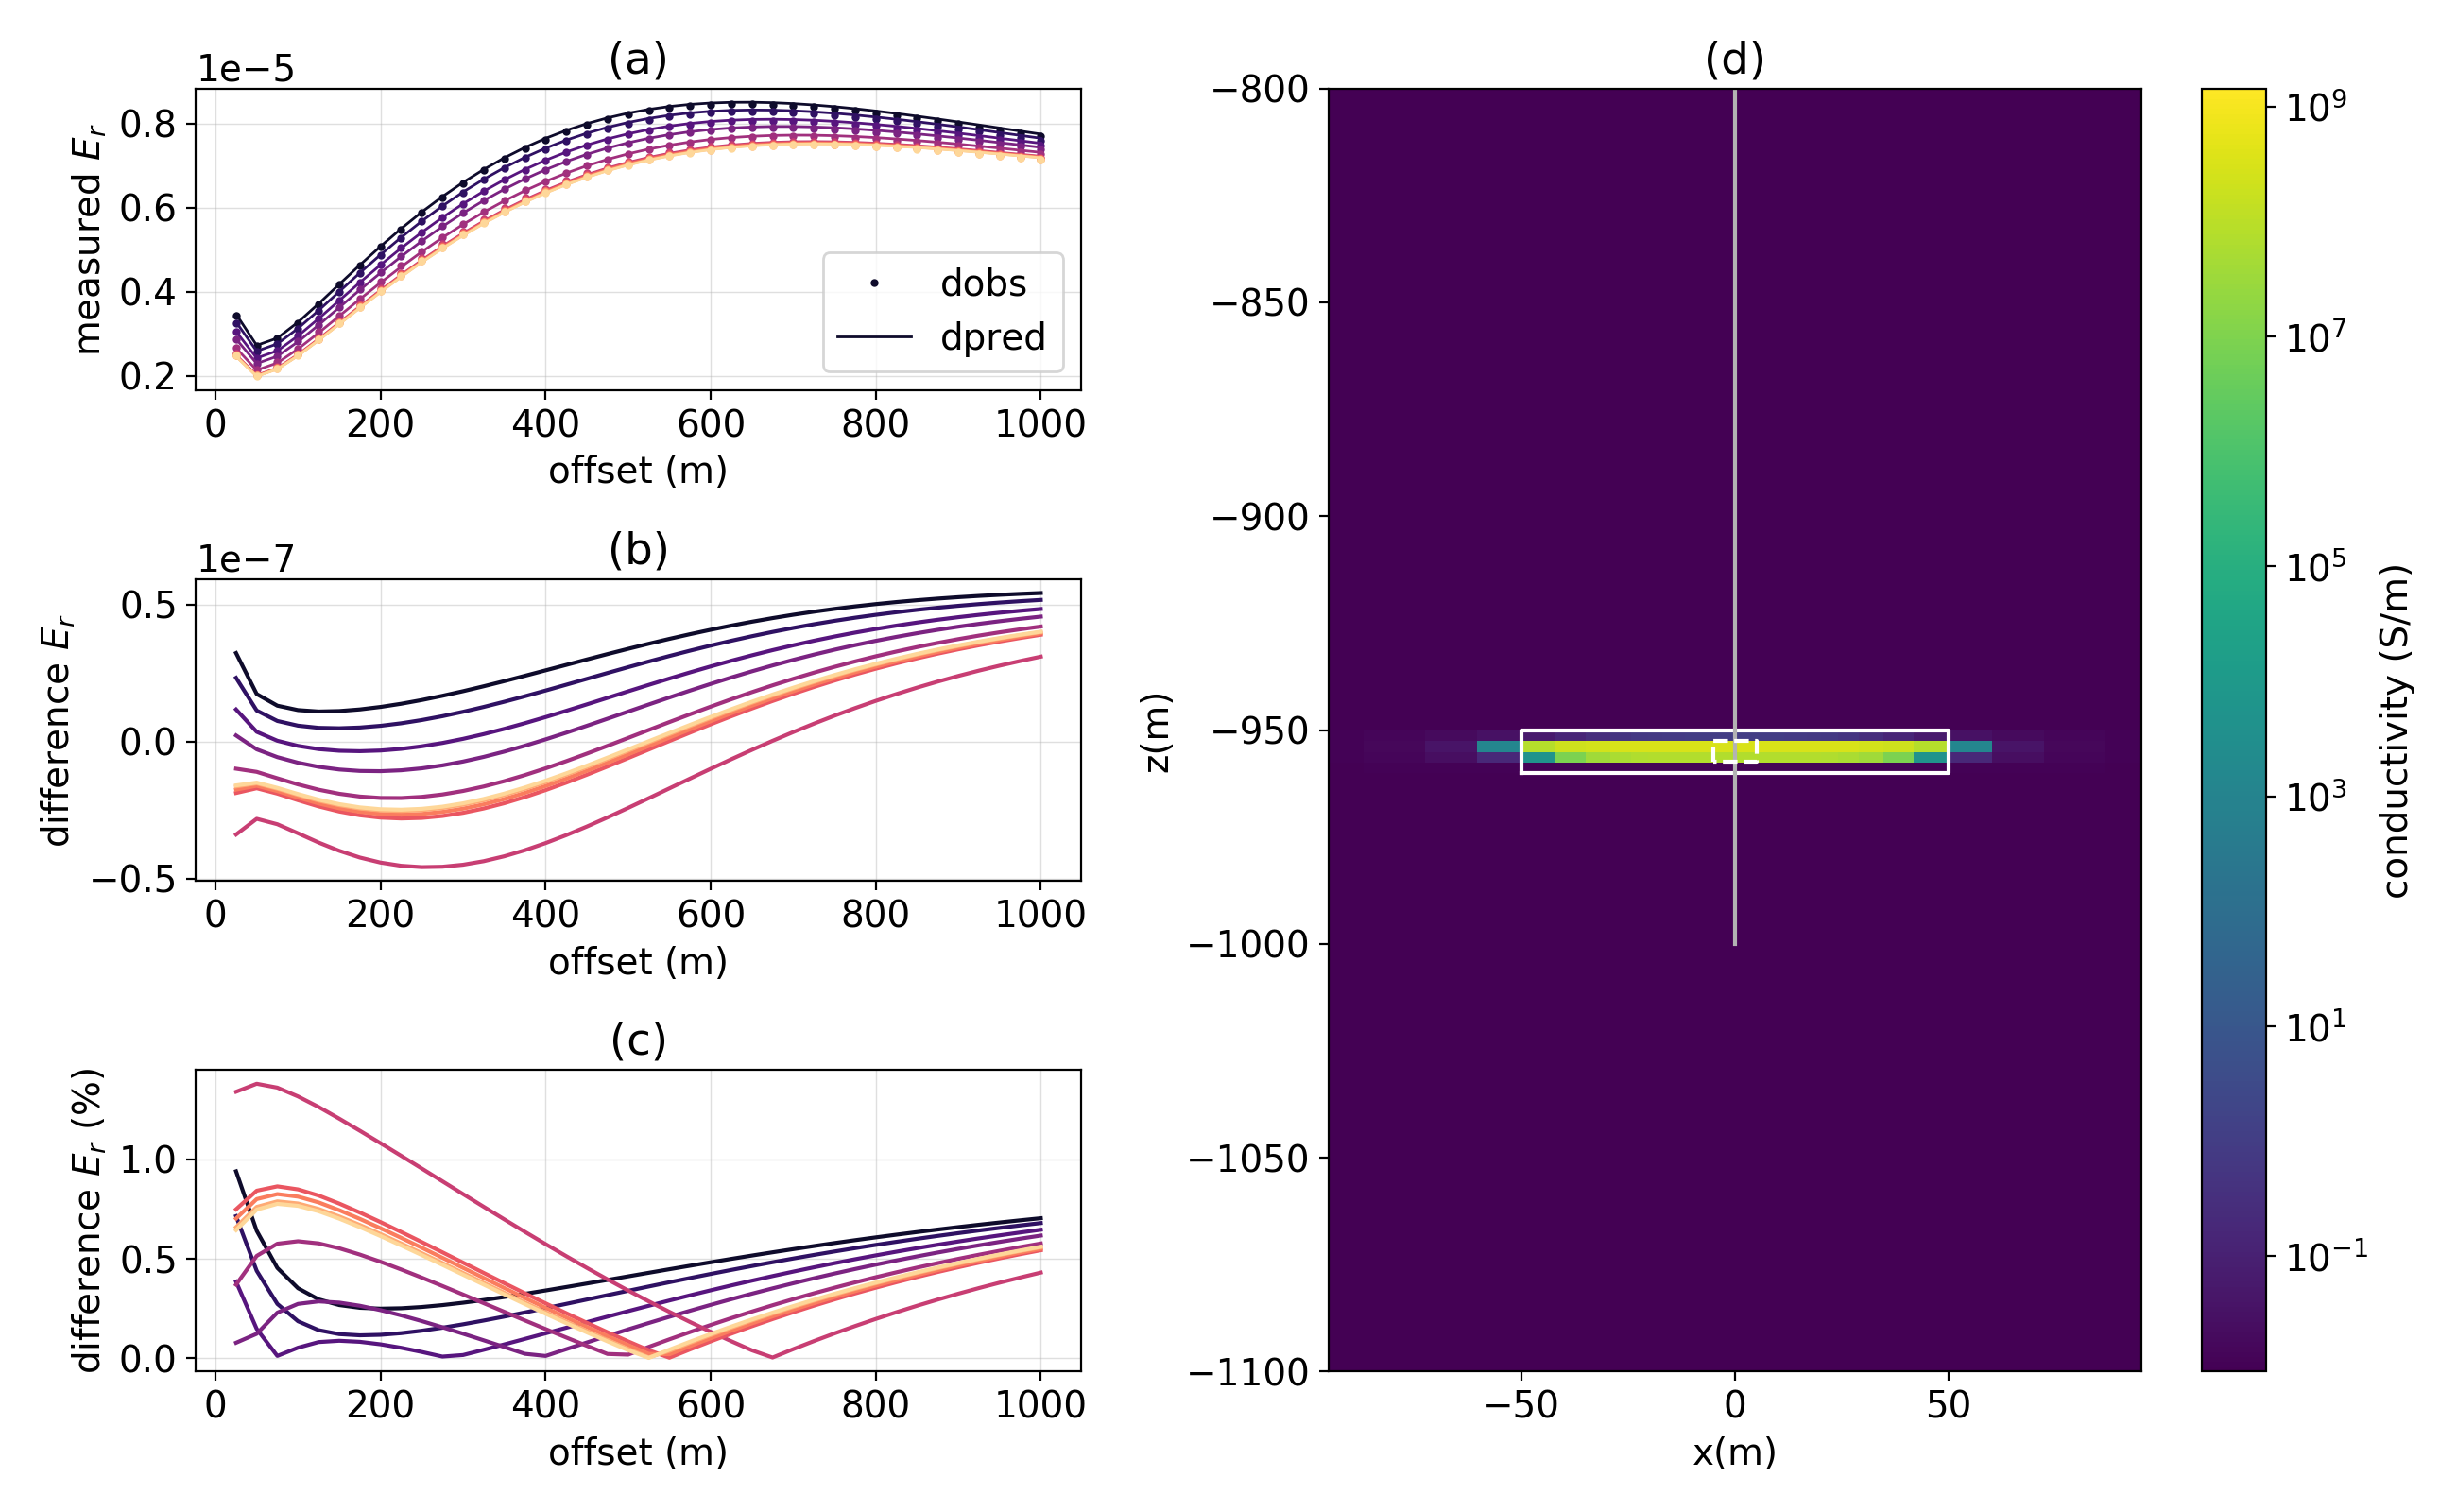
\includegraphics[width=0.8\textwidth]{figures/inversion/parametric_voxel2.png}
    \end{center}
\caption{
    Parametric inversion result for a starting model
    centered at 955m depth with a thickness of 5m and a radius of 5m. The initial background
    conductivity is $10^{-2}$ S/m and the initial conductivity of the target is $3\times10^{-2}$ S/m.
    The geometry of the starting model is shown by the white dashed-lines and the
    true model is shown by the solid white outline. The inversion reached a $\chi$-factor $<$ 0.05
    and took 8 iterations.
}
\label{fig:parametric_voxel2}
\end{figure}


The casing spreads out the source currents along its length, this may reduce sensitivity to the depth and thickness of the target. If that is the case, perhaps starting with the correct depth-center and thickness will improve the result. Figure \ref{fig:parametric_voxel2_dz10} shows the recovered model when the correct depth and vertical extent of the target are used for the starting model. The thickness of the target is closer to the true thickness. However, he conductivity is still overestimated (960 S/m), but not nearly as severely as the previous inversion. The depth has been shifted down beneath the target, and the radius (23 m) is underestimated.


\begin{figure}
    \begin{center}
    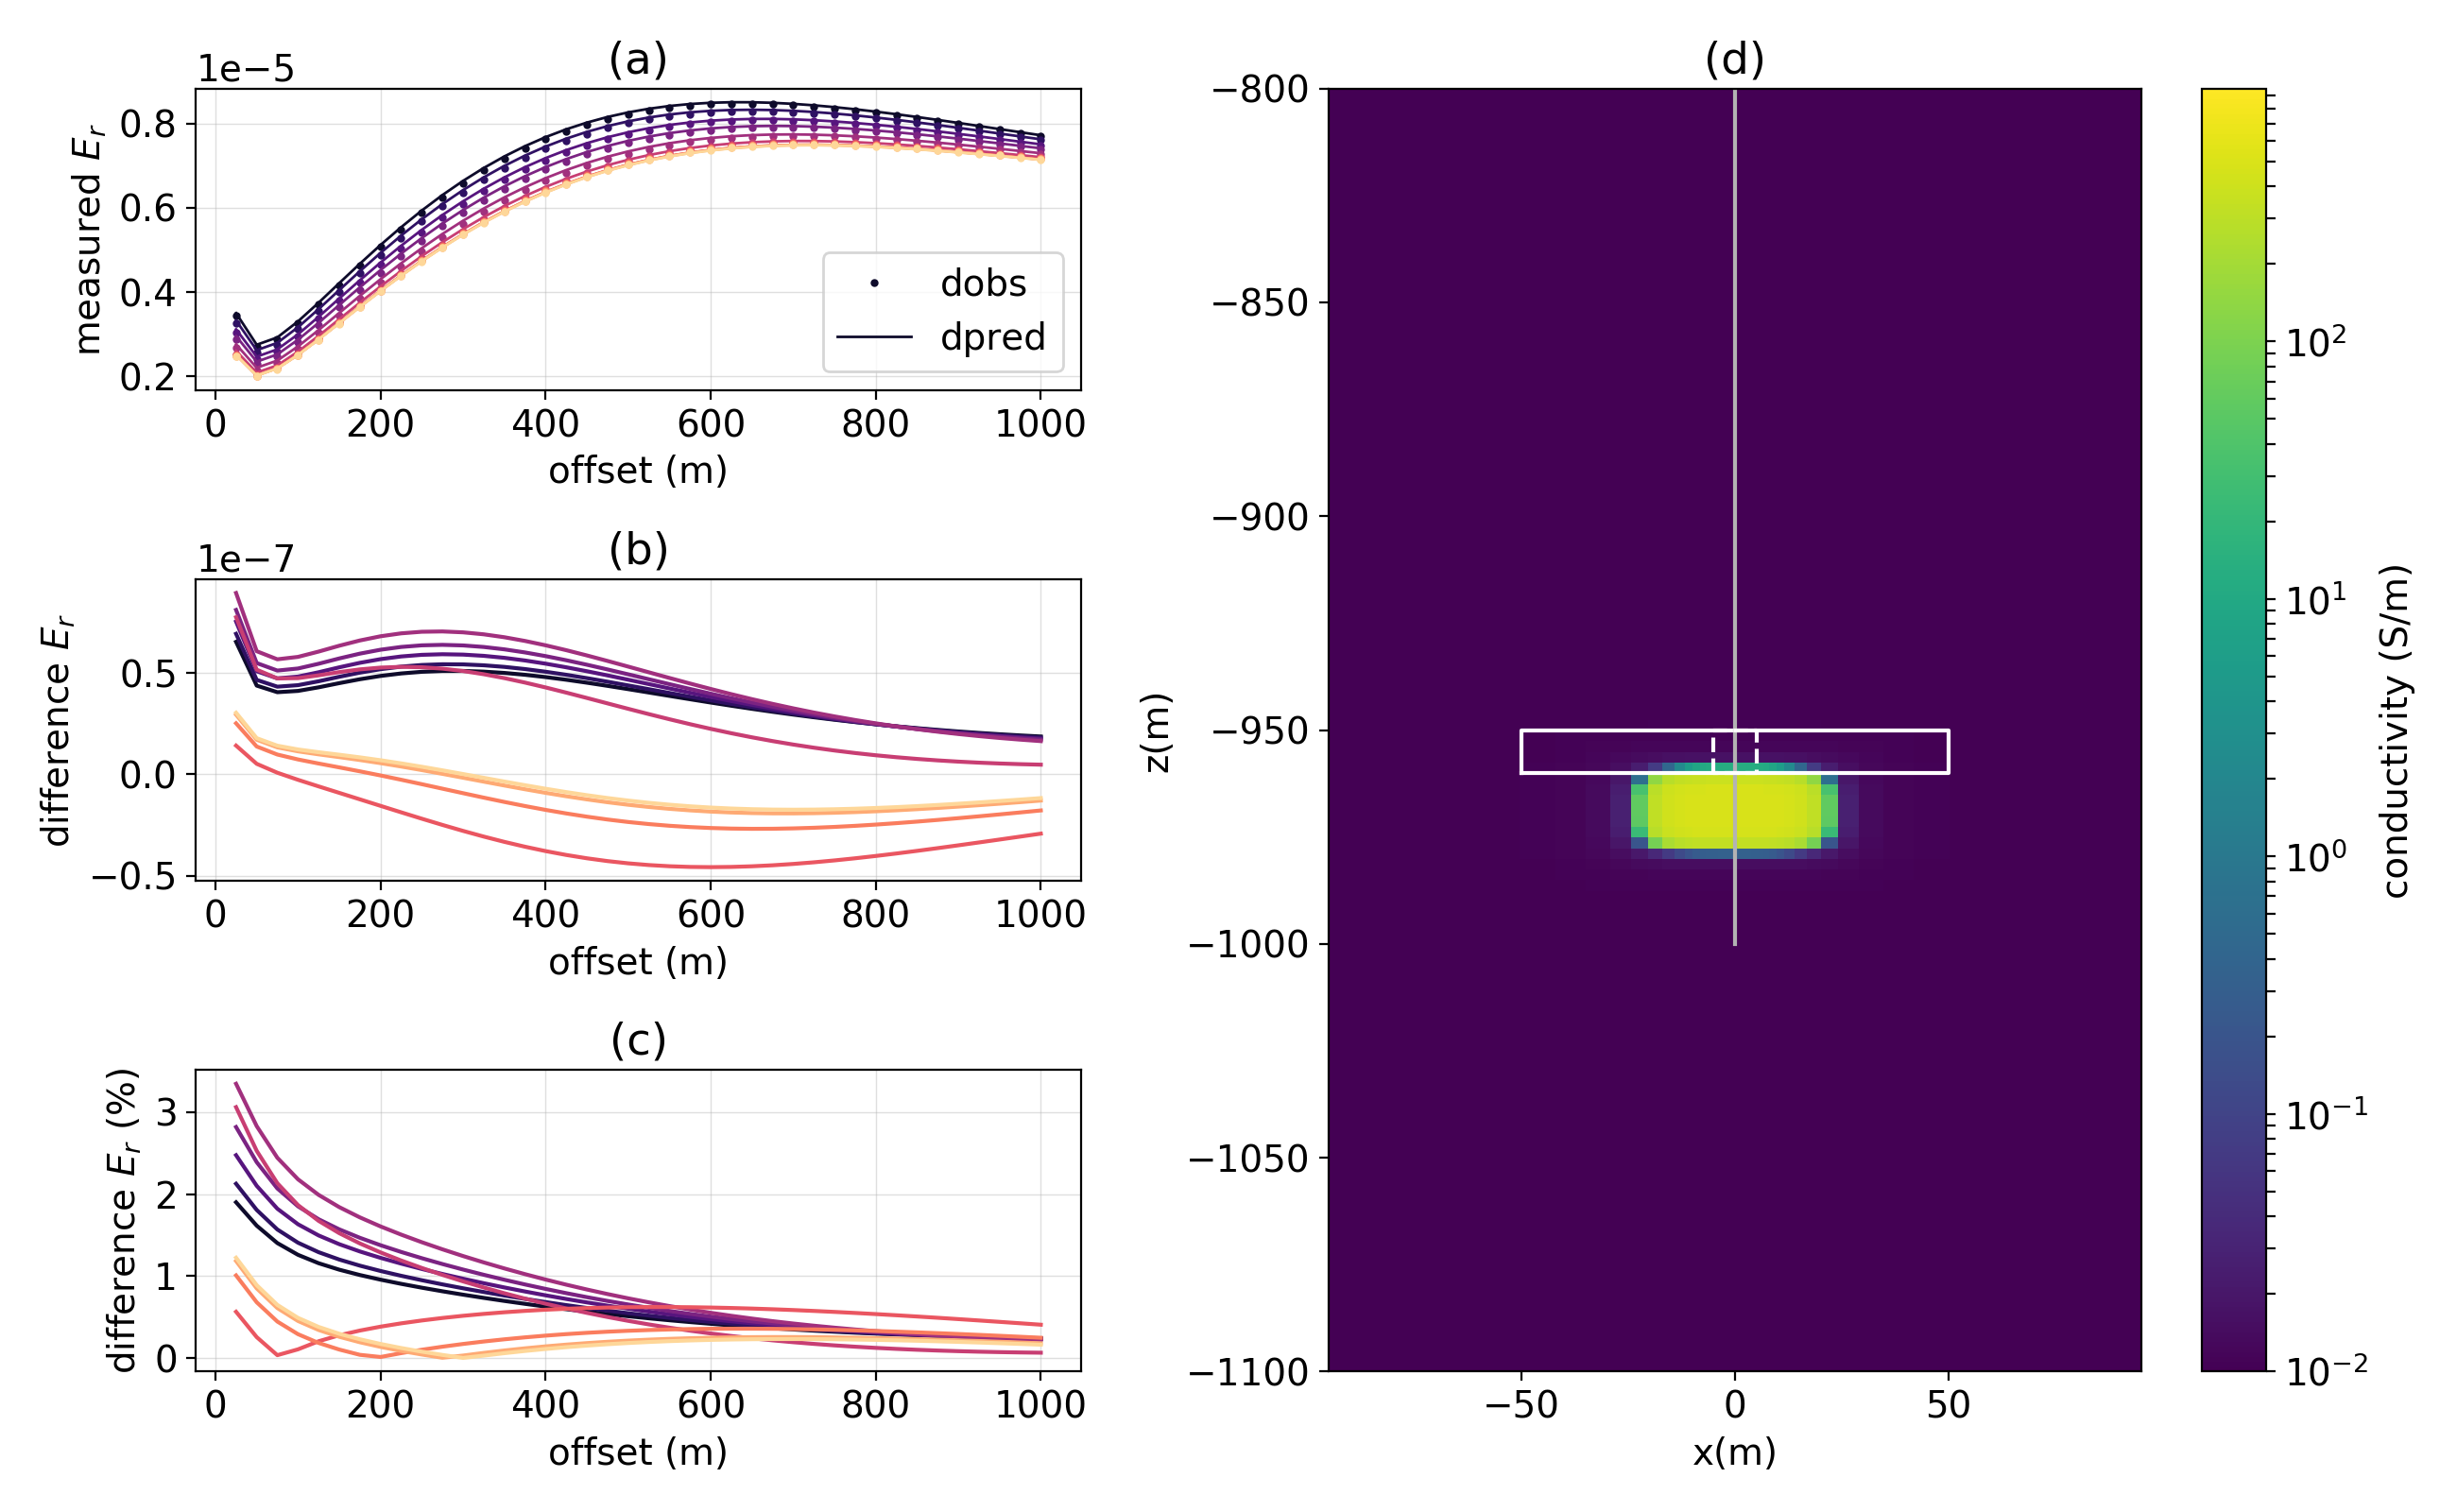
\includegraphics[width=1\textwidth]{figures/inversion/parametric_voxel2_dz10.png}
    \end{center}
\caption{
    Parametric inversion result for a starting model
    centered at 955m depth with a thickness of 10m and a radius of 10m. The initial background
    conductivity is $10^{-2}$ S/m and the initial conductivity of the target is $3\times10^{-2}$ S/m.
    The geometry of the starting model is shown by the white dashed-lines and the
    true model is shown by the solid white outline. The inversion reached a $\chi$-factor < 0.05
    and took 8 iterations.
\label{fig:parametric_voxel2_dz10}
\end{figure}


If I start the inversion closer to the true solution, for example a radius of 75 m and a thickness of 5 m, then, not surprisingly, I obtain a solution closer to the true solution. The recovered radius is 76 m, thickness is 7 m and the conductivity 2 S/m. This inversion result is shown in Figure \ref{fig:parametric_voxel2_large_r}.


\begin{figure}
    \begin{center}
    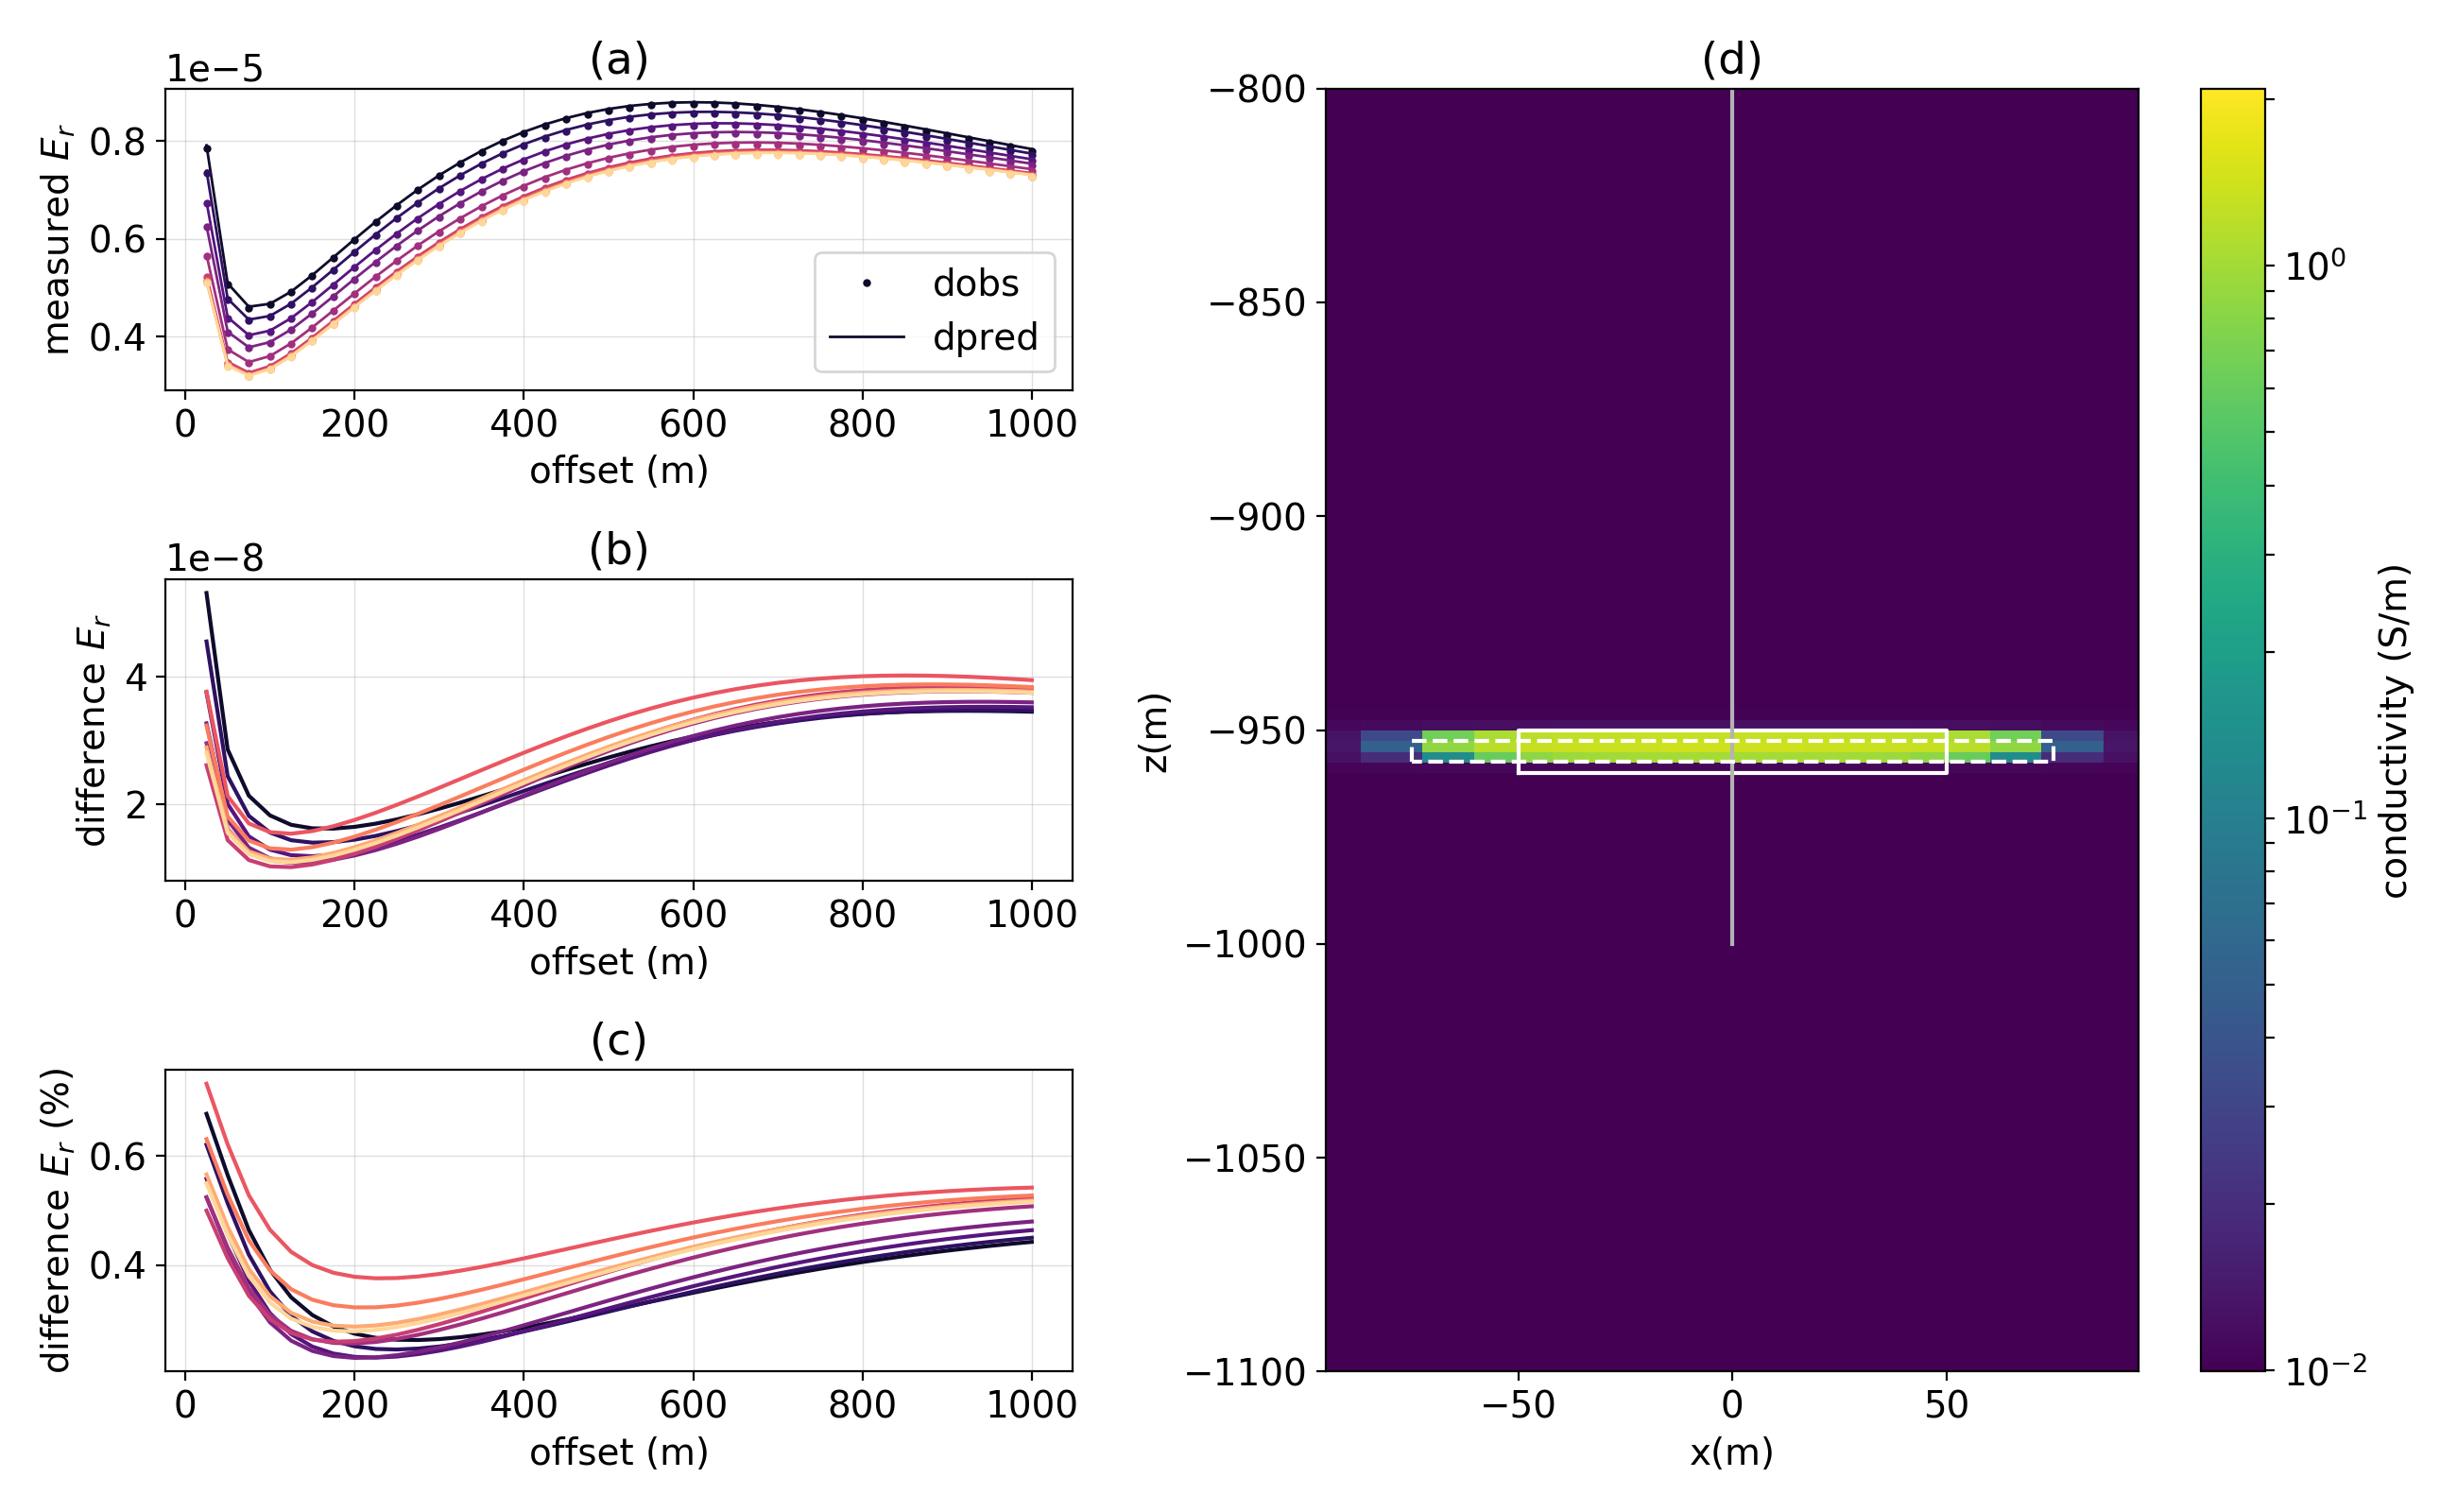
\includegraphics[width=0.8\textwidth]{figures/inversion/parametric_voxel2_large_r.png}
    \end{center}
\caption{
    Parametric inversion result where the center of the target is fixed at a depth
    of 955 m. The starting model has a thickness of 5 m and a radius of 75 m. The initial background
    conductivity is $10^{-2}$ S/m and the initial conductivity of the target is $3\times10^{-2}$ S/m.
    The geometry of the starting model is shown by the white dashed-lines and the
    true model is shown by the solid white outline. The inversion reached a $\chi$-factor $<$ 0.05
    and took 6 iterations.
}
\label{fig:parametric_voxel2_large_r}
\end{figure}


These inversion results provide some insights into the non-uniqueness of the problem. In particular, depending on the starting model, the recovered conductivity of the target can vary by many orders of magnitude. I suspect that the large conductivity of the casing is a major contributor to the difficulty of this inverse problem. The conductive casing tends to spread out the source currents, which consequently spreads out the sensitivity as compared to a point electrode. Furthermore, the currents along the casing are altered due to the presence of a conductive target -- this is a more complex interaction than typically encountered in a DC experiment.

The geometry of the parametric inversion results provides a more intuitive geometry for interpretation, but, on its own, the inversion is not particularly robust. Thus we require more a-priori information or assumptions be imposed in the inversion. There are several approaches that could be taken to try and tame the inversion: the electrical conductivity could be bounded, for example by using hard-constraints in the optimization, or a weighting scheme could be adopted to try to compensate for the sensitivities. This level of ``tuning'' in the inversion is something I wish to avoid. Instead, I will consider changing the model-space by using effective medium theory to map a volume-concentration of fractures to electrical conductivity.

\subsection{Inversion for fracture concentration}
Effective medium theory provides a mapping from a volume-concentration of fractures, $\varphi$, to electrical conductivity given known values for the conductivity of the background and the conductivity of the material filling the fractures. Instead of inverting for electrical conductivity (or log-conductivity), we can invert for a concentration of fractures. This has several important implications in the inversion. First of all, it changes the parameter space which we are working in; this affects both the regularization and the computation of the sensitivities. In addition, it provides natural bounds for the conductivity, as $0 \leq \varphi \leq 1$. Figure \ref{fig:scemt_mapping} shows the effective conductivity as a function of fracture concentration for the model considered here. Panels (a) and (b) show the effective conductivity on a linear scale, while panels (c) and (d) show the effective conductivity on a log-scale. The panels on the right (b) and (d) zoom in to lower concentrations ($0 < \varphi < 0.005$). The mapping between concentration and effective conductivity is approximately linear over the range of concentrations we expect to encounter for a fractured volume of rock. Recall that the true concentration is 0.003. In comparison, the bottom two plots, Figure \ref{fig:scemt_mapping} (c) and (d) show the log-conductivity, which is the parameter I was inverting for in previous examples. It is quite non-linear, particularly at low concentrations. Consider, for example how this manifests in the regularization. If I regularize on log-conductivity, the difference between $10^{-2}$ S/m (the background) and $1$ S/m is penalized much more significantly than the difference between 1 S/m and 2 S/m. If instead, I regularize on concentration, then the difference between $10^{-2}$ S/m and $1$ S/m is treated nearly the same as the difference between 1 S/m and 2 S/m as each corresponds to an increase in concentration by 0.001 S/m. The associated sensitivity function is shown in Figure \ref{fig:casing_sensitivity_scemt}. As compared to the log-conductivity inversion (Figure \ref{fig:casing_sensitivity}), the sensitivity is much more uniform over the length of the well for both (a, b) the halfspace and (c, d) the true models.

\begin{figure}
    \begin{center}
    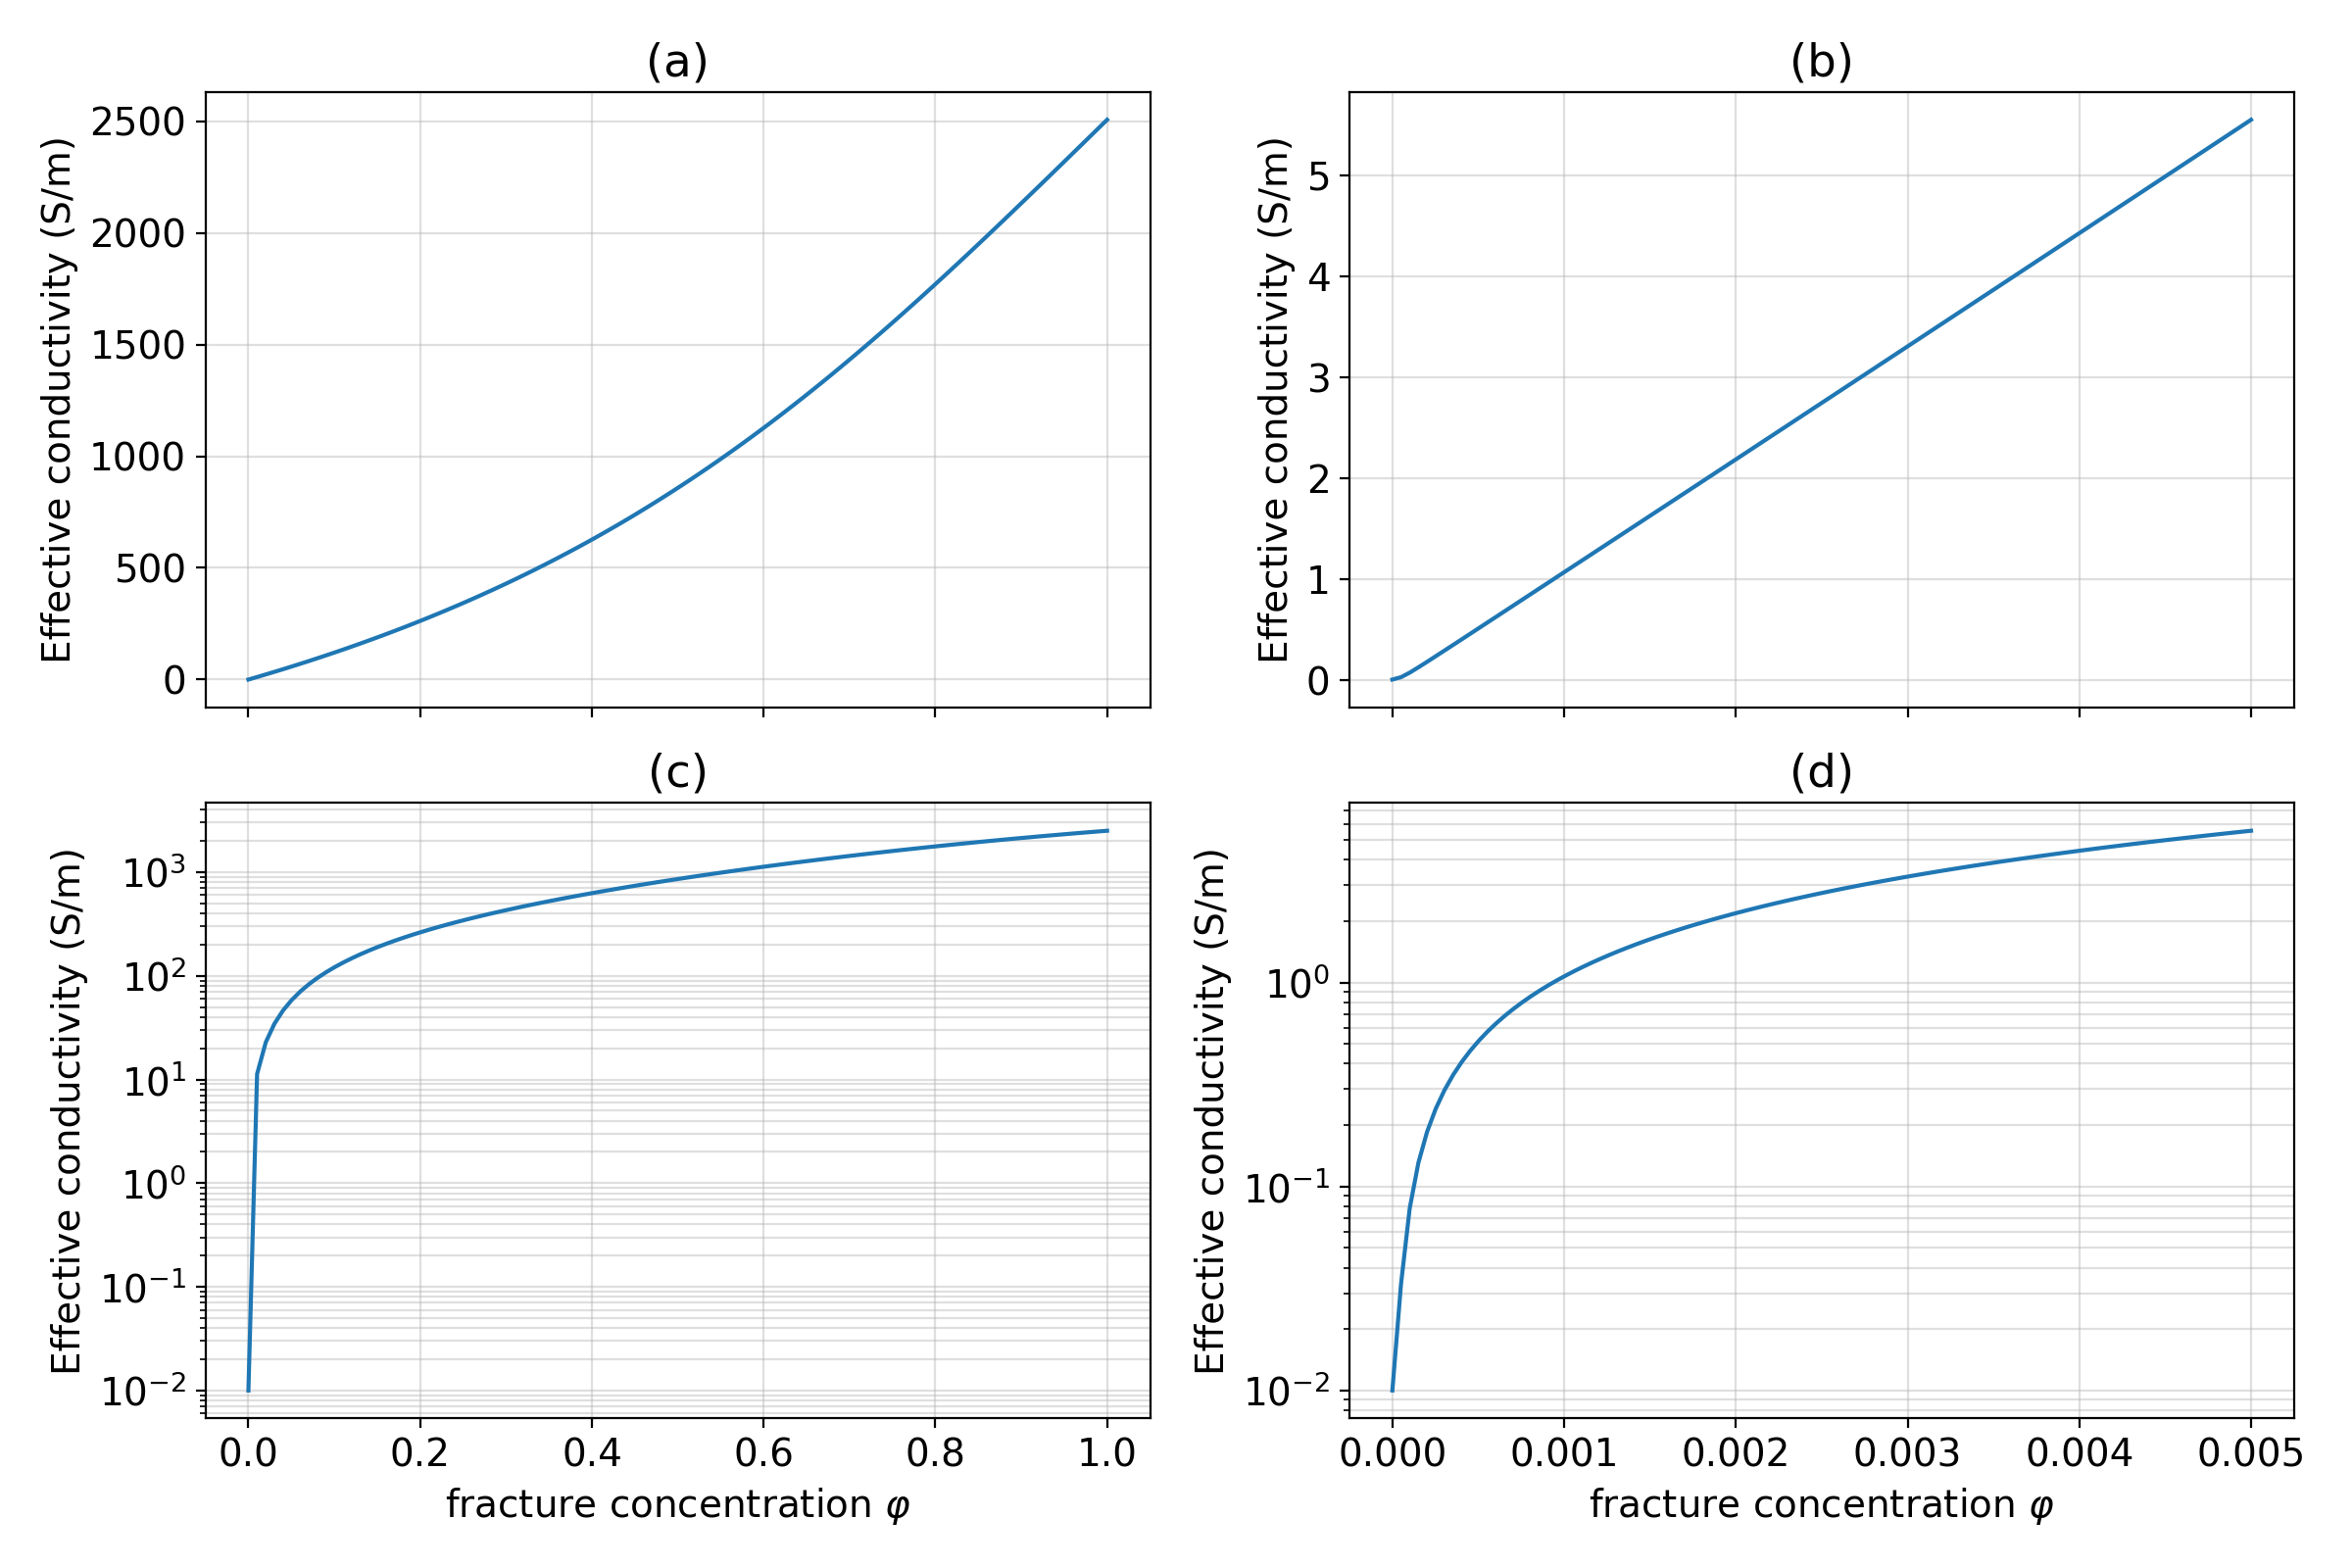
\includegraphics[width=0.8\textwidth]{figures/inversion/scemt_mapping.png}
    \end{center}
\caption{
   Self-consistent effective medium theory estimation of electrical conductivity as a function of fracture concentration.
   The conductivity of the background is $10^{-2}$ S/m and the conductivity of the material filling the fractures is 2500 S/m.
   We use an aspect ratio of $3 \times 10^{-5}$, and the fractures are assumed to be randomly oriented. Panels (a) and (b) show the
   conductivity on a linear scale while panels (c) and (d) show the conductivity on a logarithmic scale. Panels (a) and (c) show the
   full range of possible $\varphi$ values from 0 to 1, and panels (b) and (d) zoom into a smaller range, 0 $\leq \varphi \leq 0.005$.
}
\label{fig:scemt_mapping}
\end{figure}





\begin{figure}
    \begin{center}
    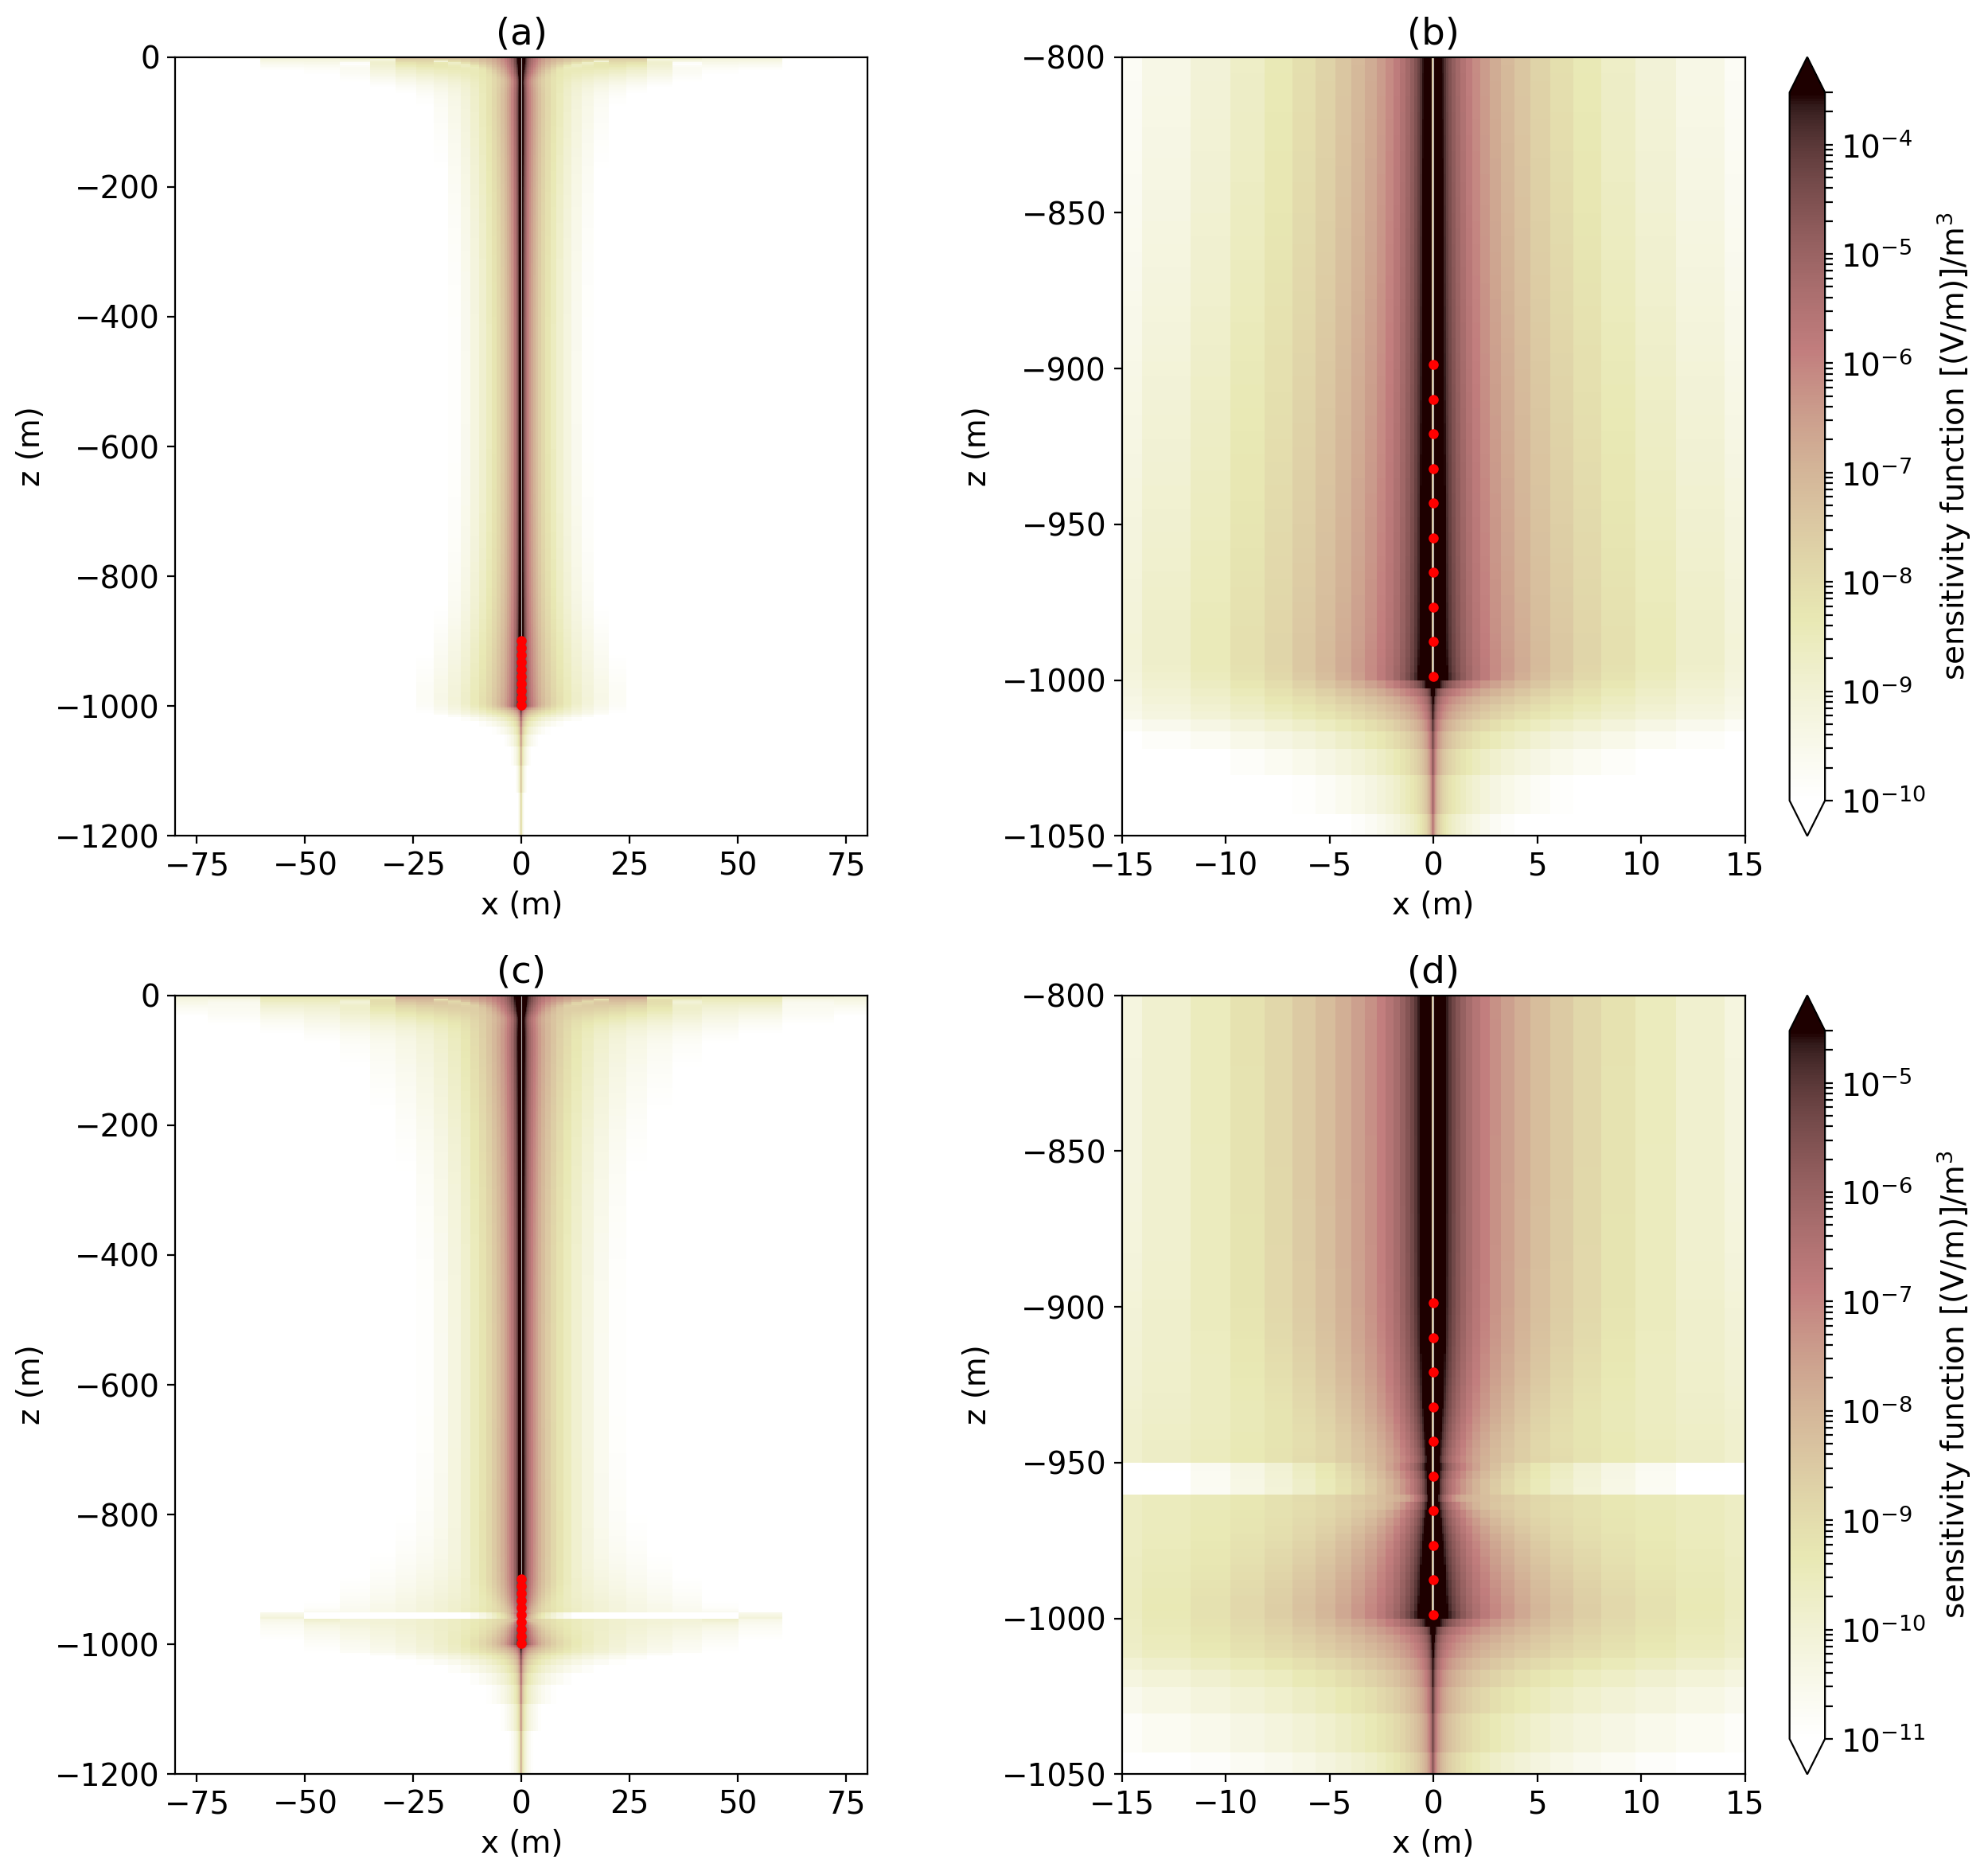
\includegraphics[width=\textwidth]{figures/inversion/casing_sensitivity_scemt.png}
    \end{center}
\caption{
    Integrated sensitivity, similar to that shown in \ref{fig:casing_sensitivity}, except here,
    the inversion model is fracture concentration.
    Panels (a, b) are the sensitivity for a $\varphi=\mathbf{0}$ half-space and
    (c, d) show the sensitivity calculated using the true model which includes the fracture.
}
\label{fig:casing_sensitivity_scemt}
\end{figure}


To examine how using an effective medium theory model parameterization impacts the inversion, I run a standard voxel inversion, as in Section \ref{sec:voxel_inversion}, but now using $\varphi$ as the inversion model. For $\sigma_0$, I use the scalar value for the background, $10^{-2}$ S/m in all cells. The initial model was set slightly above zero ($10^{-10}$) S/m so that not all model cells were starting on the lower bound of $\varphi=0$. The reference model is set to to zero. Pushing the inversion to a $\chi$-factor $<$ 0.05 gives the result shown in Figure \ref{fig:dc_smooth_inversion_phi_5e-02}. I have added an additional panel and now show both the recovered concentration model (d) and the corresponding conductivity model (e). The inversion result is quite comparable to the model obtained through a log-conductivity inversion shown in Figure \ref{fig:dc_smooth_inversion_5e-02}. The main notable difference is that there is no region in which the conductivity of the background is underestimated; by bounding the concentration between 0 and 1, there is no mechanism for the inversion to reduce the conductivity.


\begin{figure}
    \begin{center}
    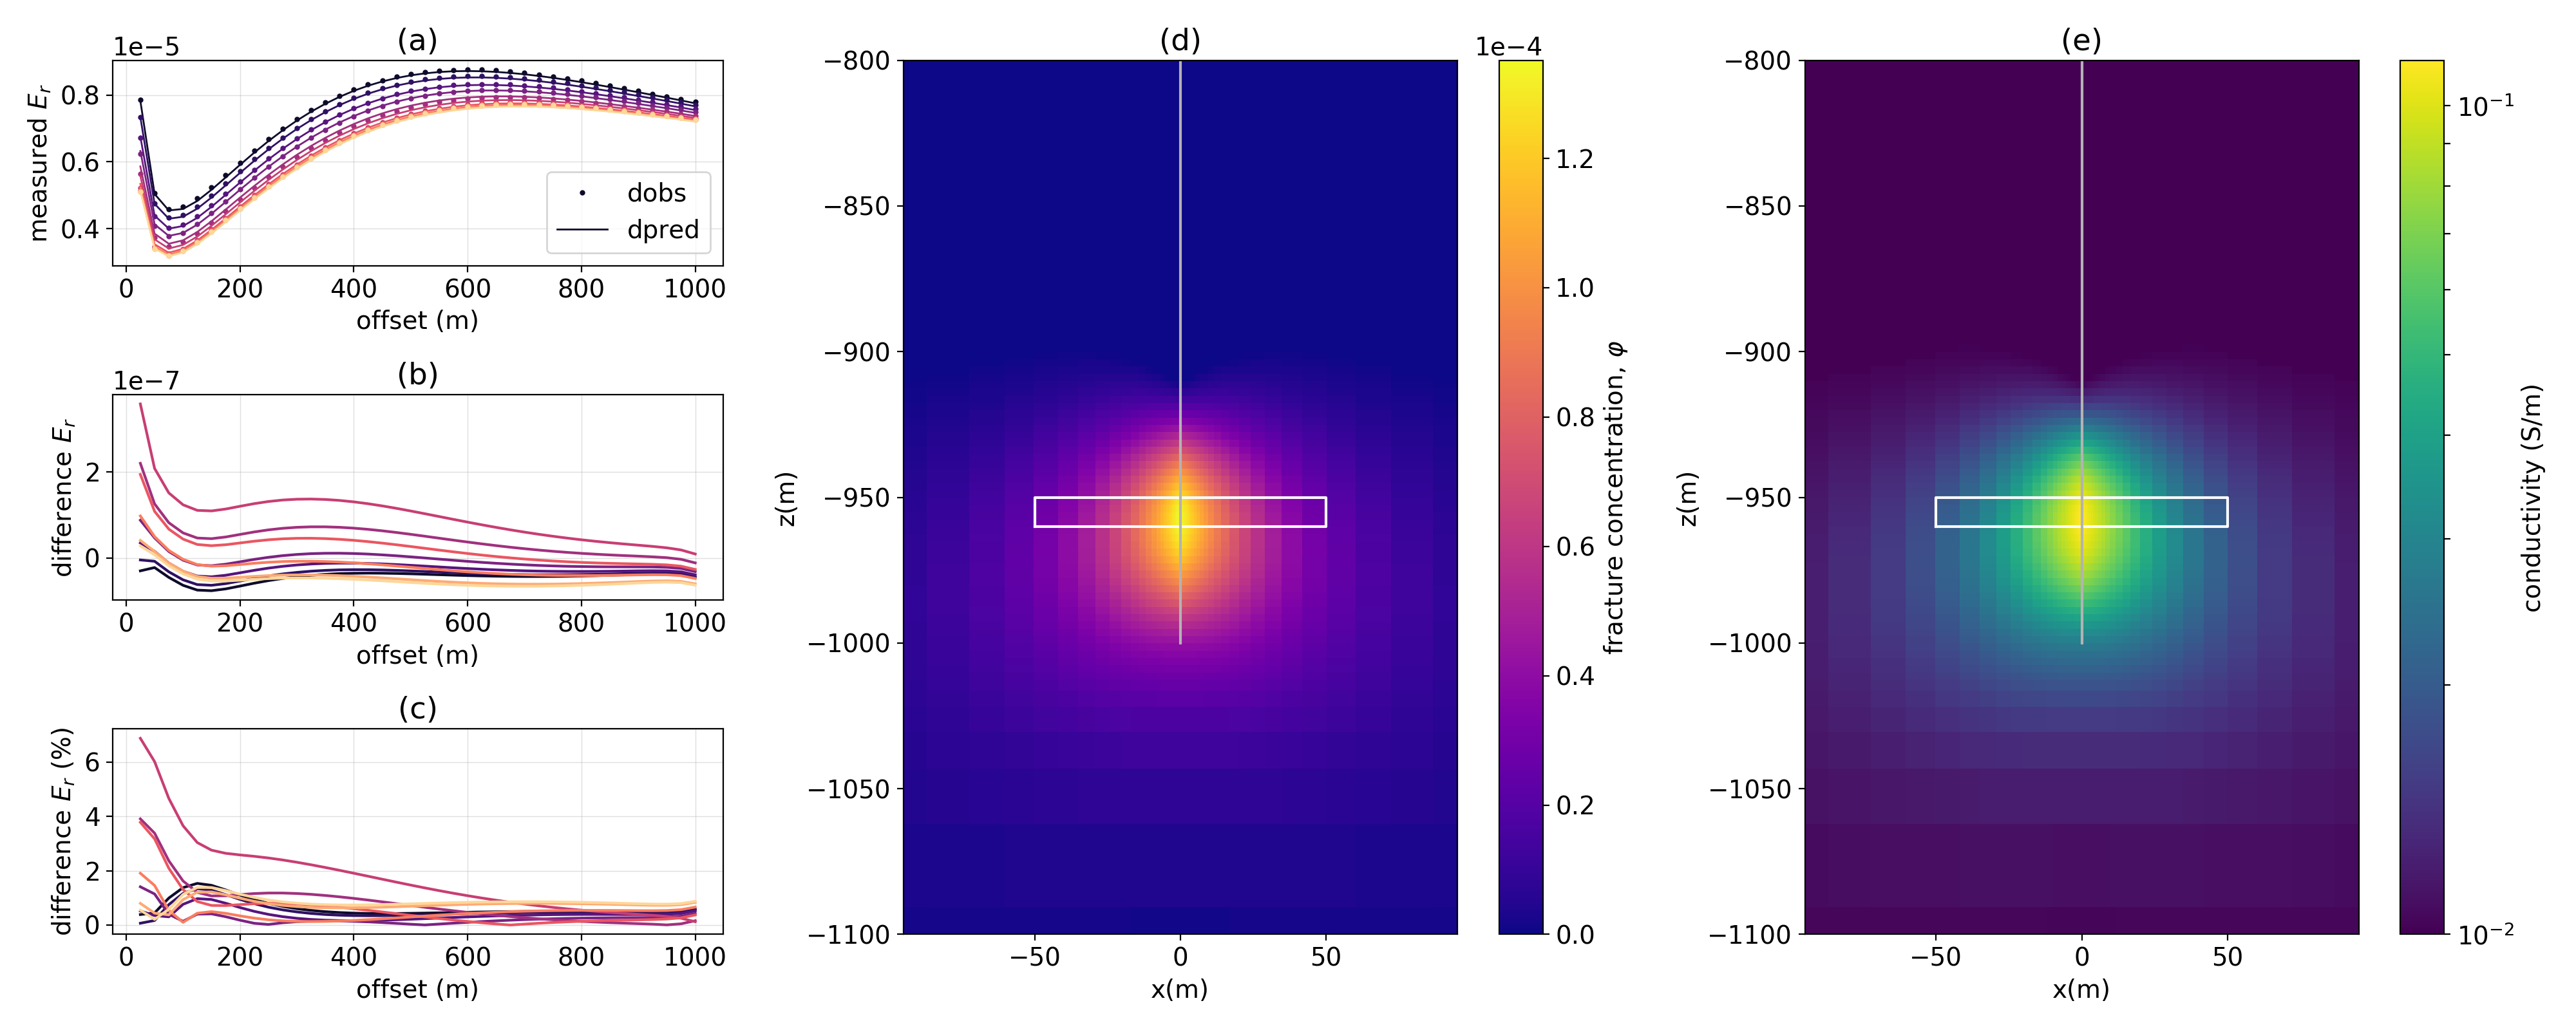
\includegraphics[width=\textwidth]{figures/inversion/dc_smooth_inversion_phi_5e-02.png}
    \end{center}
\caption{
    (a) Observed and predicted radial electric field data,
    (b) difference between the observed and predicted data (V/m),
    (c) difference between the observed and predicted data as a percentage of the observed data,
    (d) fracture concentration model, $\varphi$, recovered in the inversion, and
    (e) electrical conductivity model obtained by converting $\varphi$ to electrical conductivity using equation \ref{eq:effective_medium_theory_mapping}
    The colors in (a), (b), and (c) indicate the source location as shown in Figure \ref{fig:dc_casing_initial_data}.
    The white outline in (d) outlines the true geometry of the fracture zone and the grey line shows the location of the wellbore.
    The data are fit to a global $\chi$-factor $<$ 0.05 and the inversion took 5 iterations.
}
\label{fig:dc_smooth_inversion_phi_5e-02}
\end{figure}


Next, I consider combining the effective medium theory map with the parametric map. I invert for the volume concentration of fractures in the background and within the target as well as the depth, vertical extent and radius of the target. Similar to the starting model used to obtain the inversion result in Figure \ref{fig:parametric_voxel2_dz10}, I start with a target at the correct depth and with the correct thickness; its radius is 10 m. For a starting $\varphi$-values, I use $10^{-10}$ in the background and $10^{-4}$ in the target. In comparison to the parametric inversions for log-conductivity, the fracture concentration, and thus electrical conductivity are much closer to the range we are expecting. The recovered concentration within the target is $4\times10^{-4}$ and its conductivity is 0.3 S/m. The vertical extent is 37 m which is an overestimate, and its radial extent is 22 m, which is an underestimate. This result closely resembles the voxel model shown in \ref{fig:dc_smooth_inversion_phi_5e-02} and thus provides some evidence that using effective medium theory may be a more robust approach to the parametric inversion.


\begin{figure}
    \begin{center}
    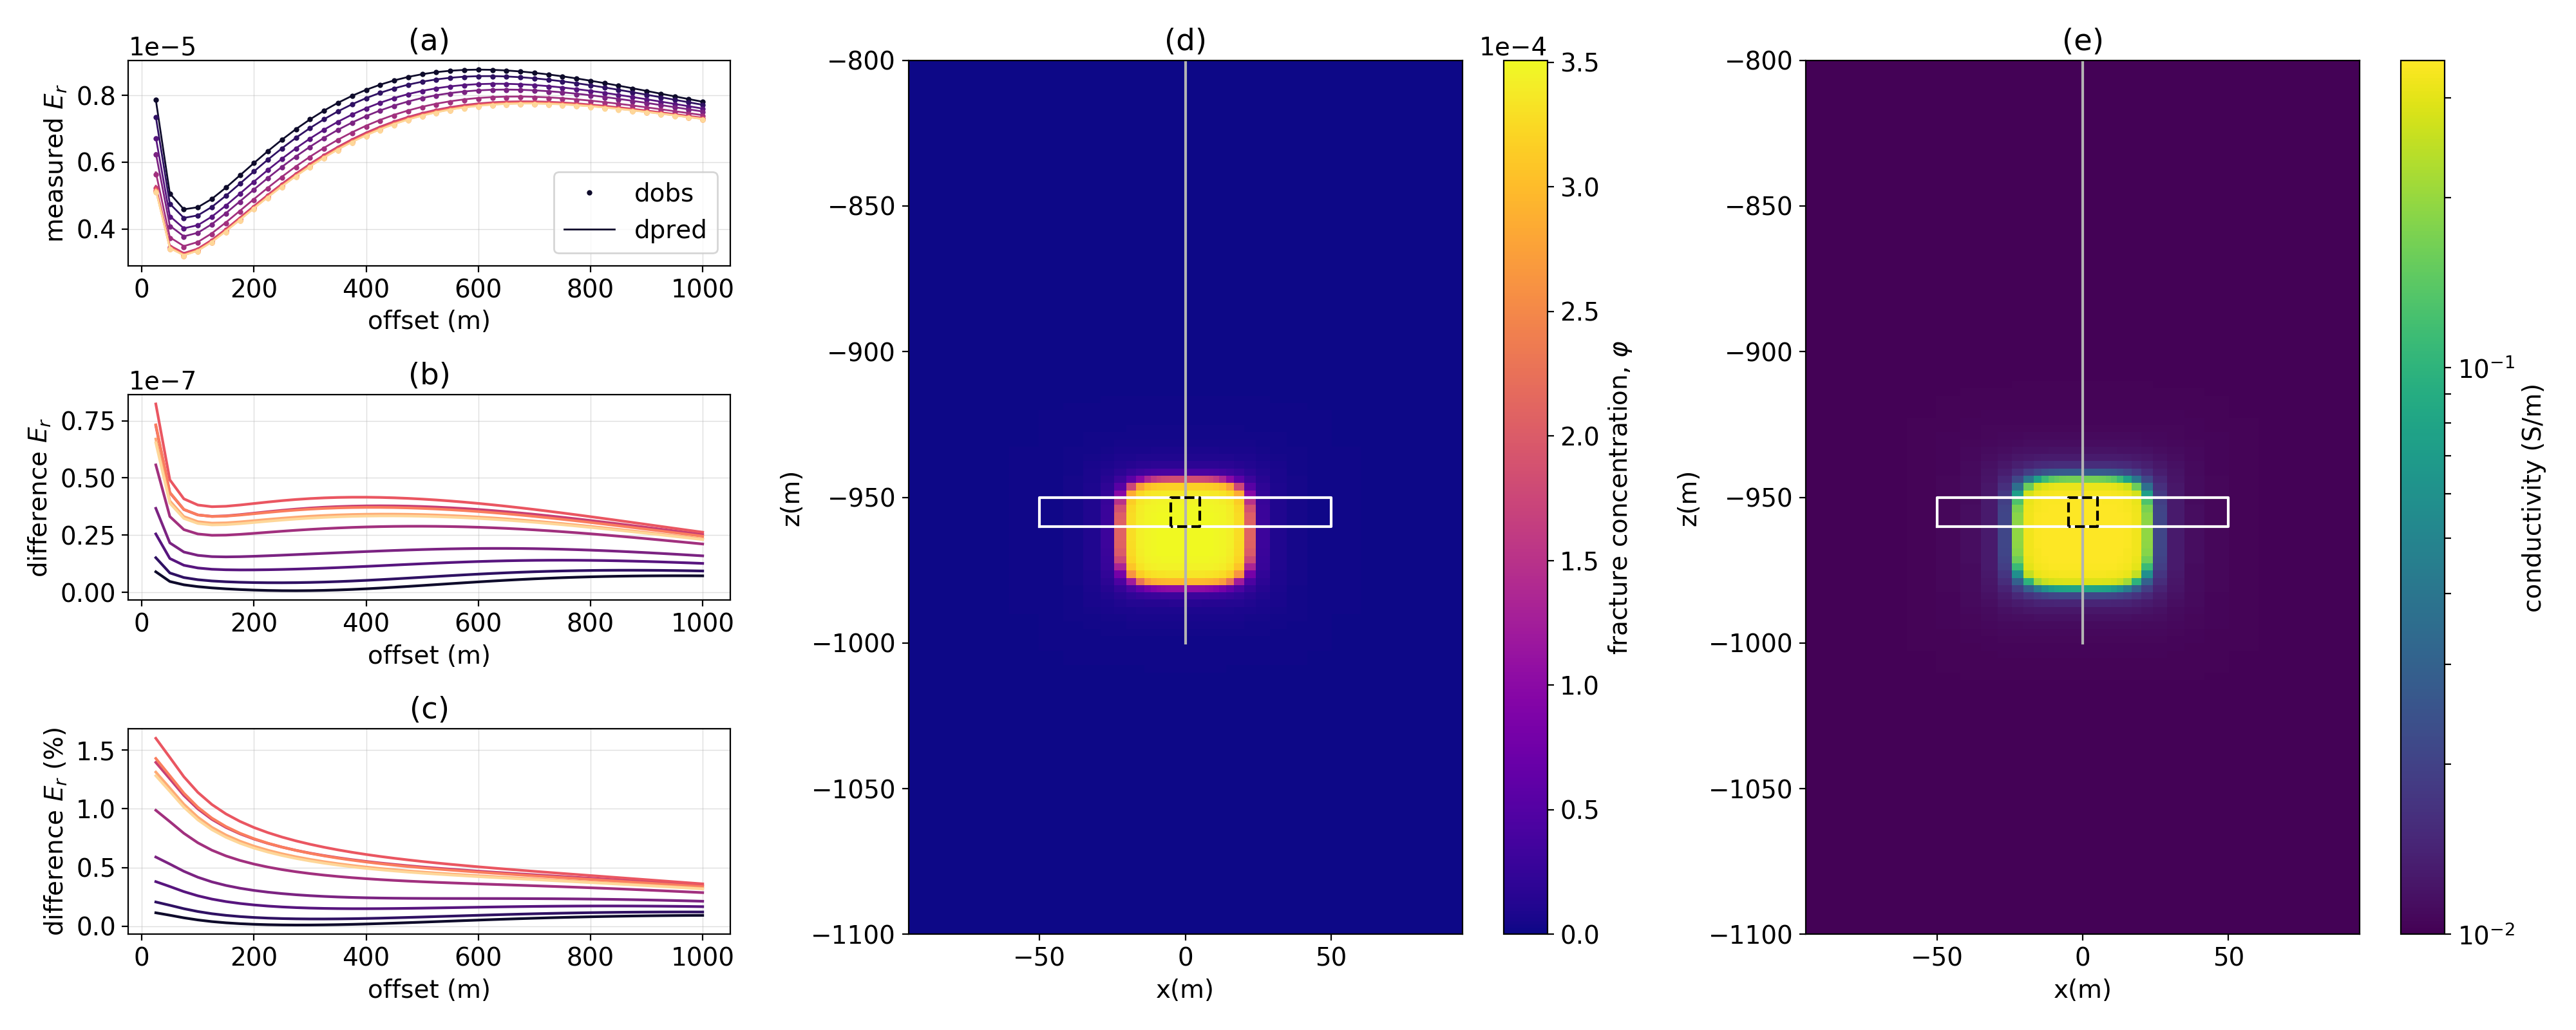
\includegraphics[width=\textwidth]{figures/inversion/dc_parametric_inversion_phi_correctz0_dz.png}
    \end{center}
\caption{
    Inversion result using a parametric model of the fracture concentration.
    The black dashed line outlines the geometry of the starting model. The initial fracture concentration
    is $10^{-10}$ in the background and $10^{-4}$ in the target.
    The data are fit to a global $\chi$-factor $<$ 0.05 and the inversion took 11 iterations.
}
\label{fig:dc_parametric_inversion_phi_correctz0_dz}
\end{figure}


Experimentation shows that using effective medium theory in combination with the parametric inversion is less sensitive to the starting model. For example, starting with a thin target as in Figure \ref{fig:parametric_voxel2} (which resulted in a conductivity of $10^{10}$ S/m for the target), I obtain the inversion result shown in Figure \ref{fig:dc_parametric_inversion_phi_correctz0}. The recovered concentration is $5 \times 10^{-4}$ S/m, which corresponds to a conductivity of 0.5 S/m. Its vertical extent is 39 m, and its radial extent is 29 m. Although there are some differences between the results obtained in Figures \ref{fig:dc_parametric_inversion_phi_correctz0_dz} and \ref{fig:dc_parametric_inversion_phi_correctz0}, these are quite minor, and are not nearly as dramatic as the models obtained by inverting for log-conductivity. Note that no regularization is used here, the difference that the effective medium theory mapping makes in the parametric inversion is in its impact on the sensitivities as well as the bounds it imposes on the conductivity. In particular, the modification of the sensitivity seems to be the main contributing factor. As the inversion progressed, the fracture concentration within the target never reached the upper bound.


\begin{figure}
    \begin{center}
    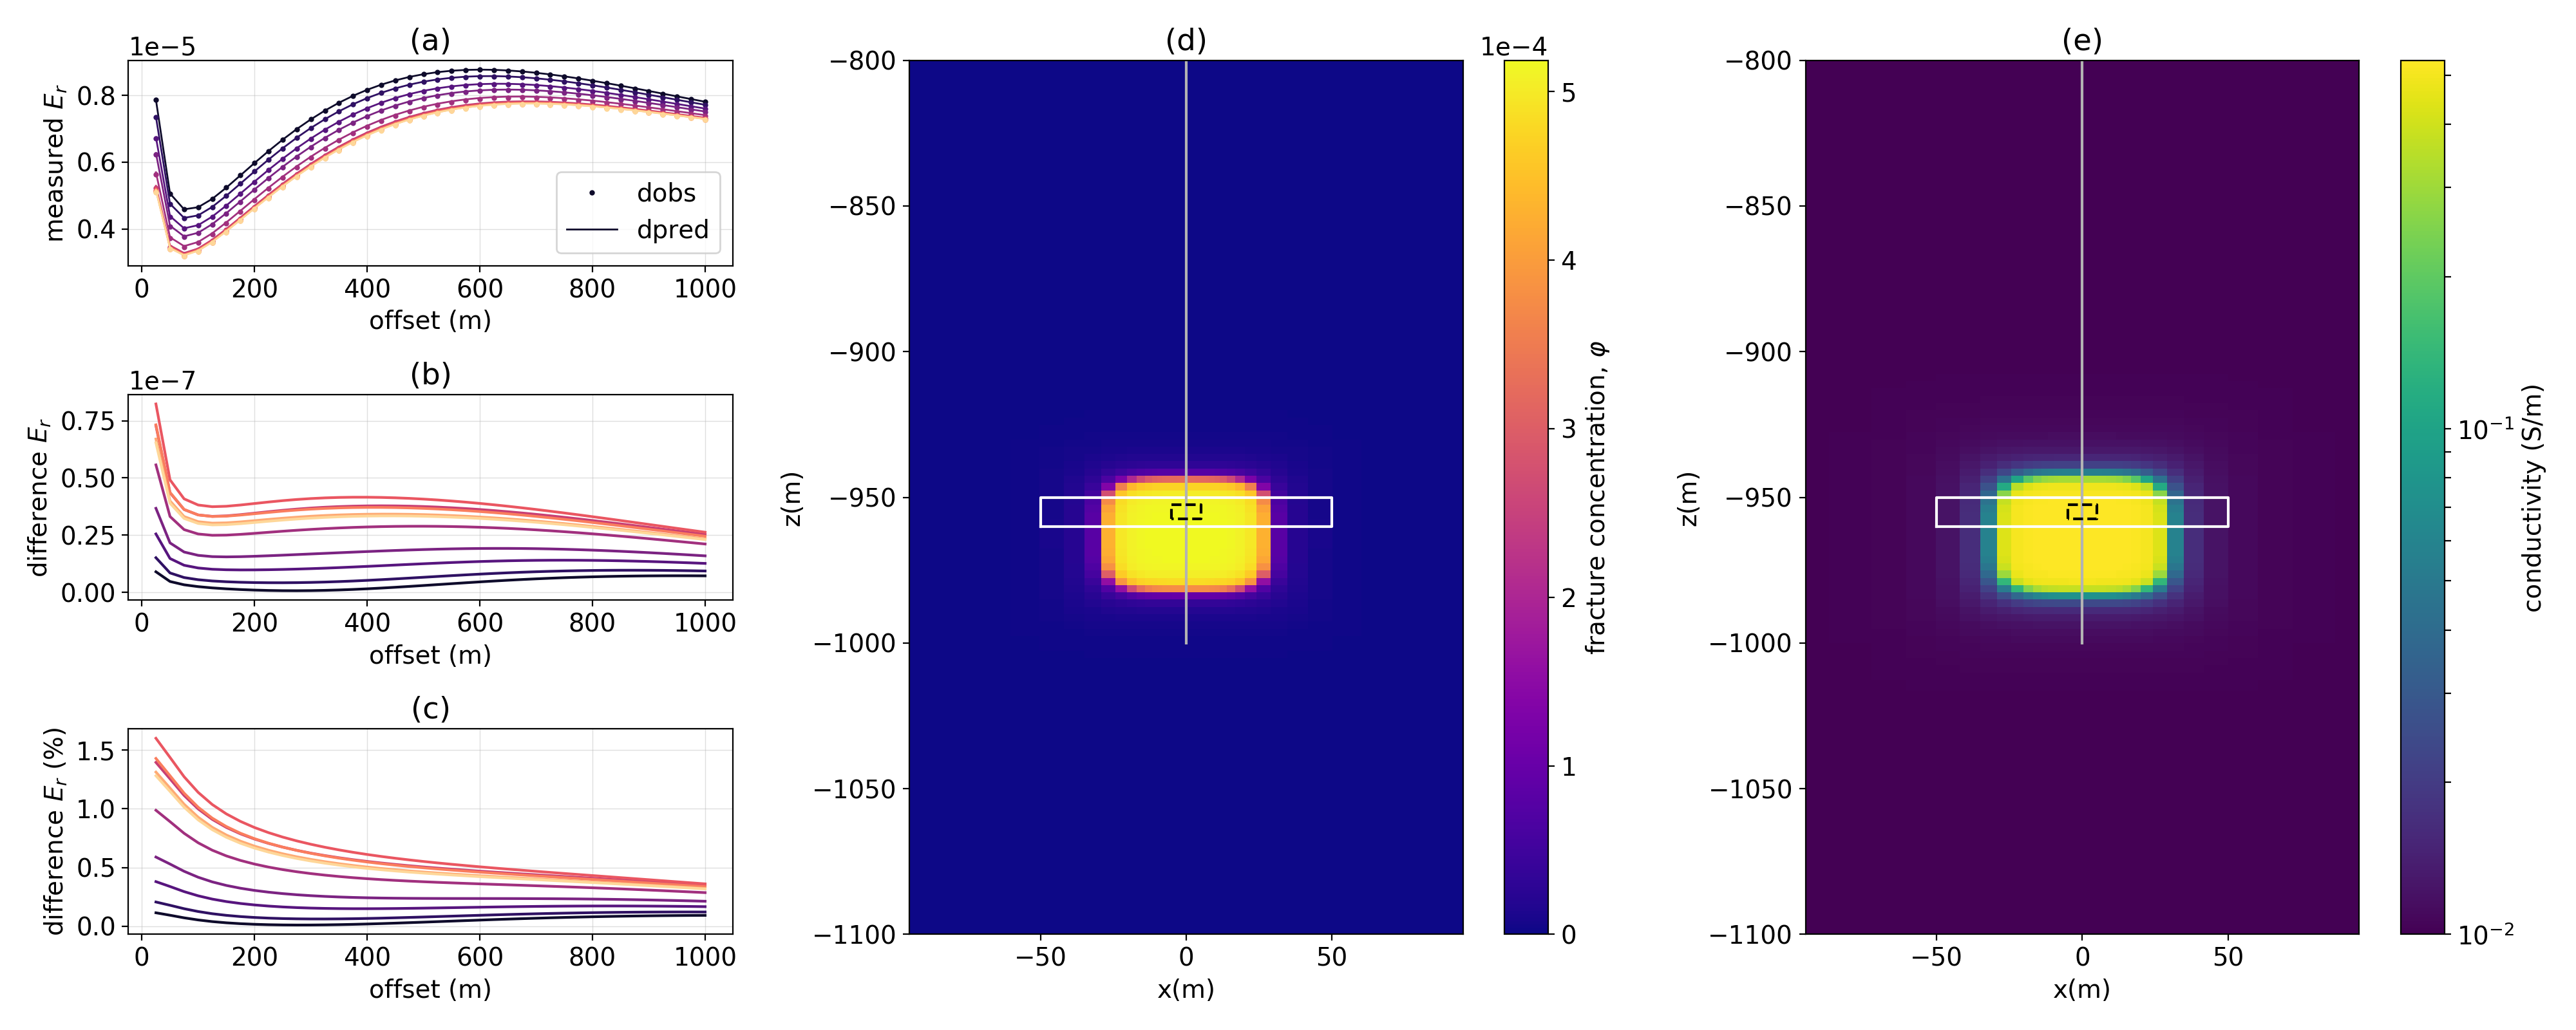
\includegraphics[width=\textwidth]{figures/inversion/dc_parametric_inversion_phi_correctz0.png}
    \end{center}
\caption{
    Inversion result using a parametric model of the fracture concentration. The concentration is
    converted to electrical conductivity using the effective medium theory mapping shown in
    equation \ref{eq:effective_medium_theory_mapping}.
    The black dashed line outlines the geometry of the starting model. The initial fracture concentration
    is $10^{-10}$ in the background and $10^{-4}$ in the target.
    The data are fit to a global $\chi$-factor $<$ 0.05 and the inversion took 12 iterations.
}
\label{fig:dc_parametric_inversion_phi_correctz0}
\end{figure}



For the DC problem, it seems that there is an element of non-uniqueness between the vertical thickness of the target and its radial extent. Starting the inversion with a geometry closer to the true solution, as in Figure \ref{fig:parametric_voxel2_large_r}, results in the model shown in Figure \ref{fig:dc_parametric_inversion_phi_correctz0_large_r}. The recovered concentration is $10^{-3}$, which corresponds to a conductivity of 1 S/m. The recovered radius is 75 m and thickness is 7 m. This indicates that in order to obtain meaningful inversion results, we will need to start in the correct proximity to the solution. For example, if the fracture was monitored with microseismic, then the volume interpreted with microseismic, which is likely an overestimate of the extent of the propped volume, could be used as a starting model.




\begin{figure}
    \begin{center}
    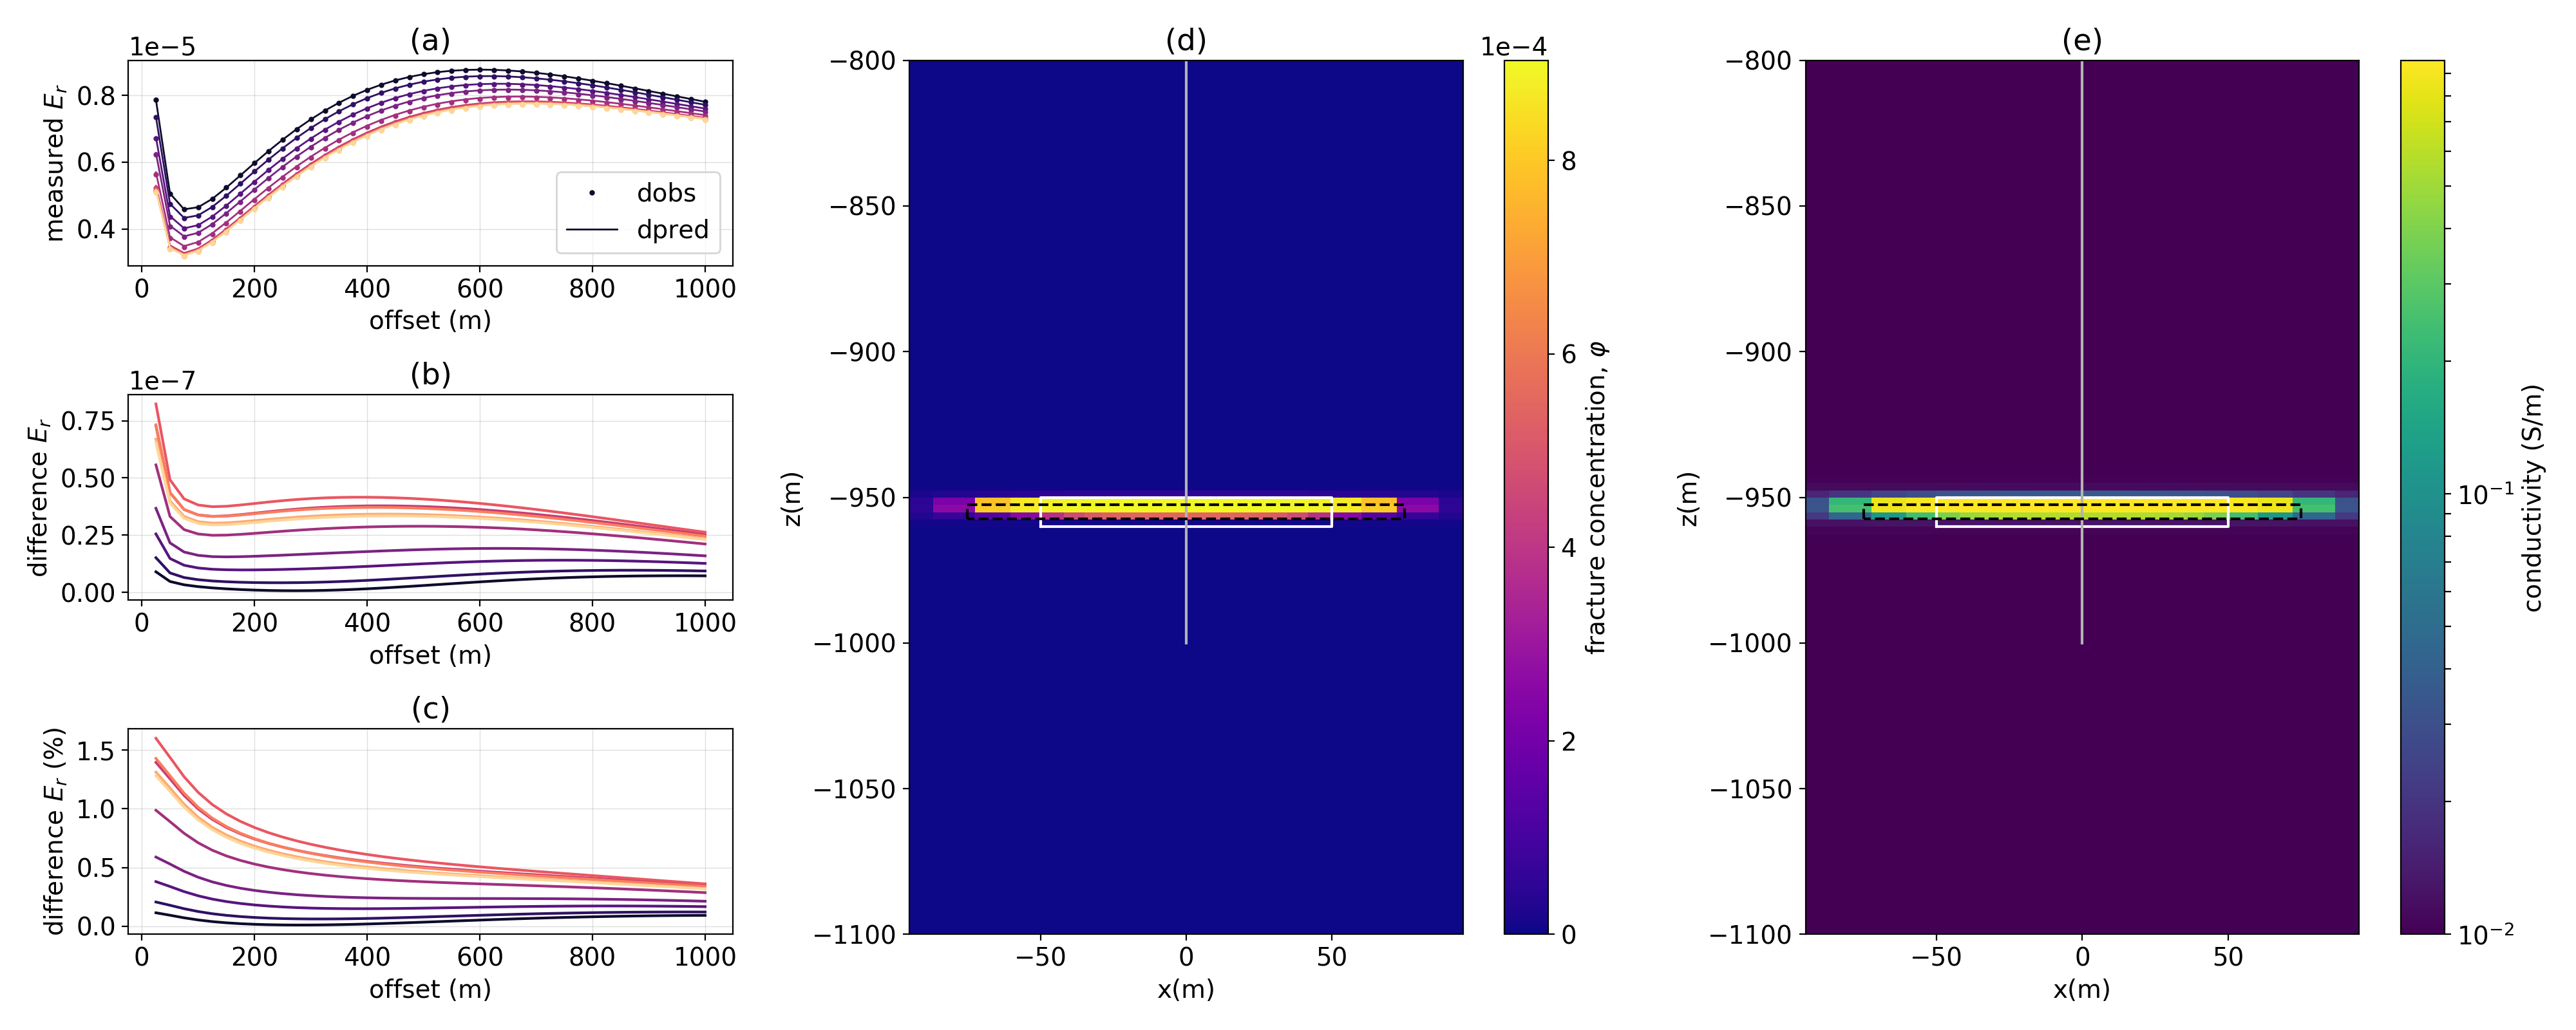
\includegraphics[width=\textwidth]{figures/inversion/dc_parametric_inversion_phi_correctz0_large_r.png}
    \end{center}
\caption{
    Parametric inversion result where the center of the target is fixed at a depth
    of 955m. The concentration is
    converted to electrical conductivity using the effective medium theory mapping shown in
    equation \ref{eq:effective_medium_theory_mapping}.
    The black dashed line outlines the geometry of the starting model. The initial fracture concentration
    is $10^{-10}$ in the background and $10^{-4}$ in the target.
    The data are fit to a global $\chi$-factor $<$ 0.05 and the inversion took 6 iterations.
}
\label{fig:dc_parametric_inversion_phi_correctz0_large_r}
\end{figure}




These inversions did not take advantage of the known volume of proppant and fluid (235 m$^3$). The inversion result in Figure \ref{fig:dc_parametric_inversion_phi_correctz0_dz} underestimates the volume at 88 m$^3$. Coincidentally, the inversion result in Figure \ref{fig:dc_parametric_inversion_phi_correctz0} comes quite close to the true volume,
226 m$^3$. The inversion which we might expect the best performance of, as its geometry is closest to the true fracture, is that in Figure \ref{fig:dc_parametric_inversion_phi_correctz0_large_r}; this inversion overestimates the volume by a factor of two: 471 m$^3$. In the next section, I examine if the inversion results can be improved by including a-priori knowledge of the volume of injected material.

\subsection{Adding a-priori volume information}
Provided that we have an estimate of the total volume of injected material (which accounts for leak-off of fluid), as well as an estimate of the relationship between the concentration of the injected material and the electrical conductivity, then the total volume can be treated as a datum in the inversion, as described in Section \ref{sec:emt_mapping}. In the following inversions, I include the volume data-misfit term (equation \ref{eq:volume_data_misfit}) in the statement of the inverse problem:
\begin{equation}
    \phi_d = \phi_{DC} + \phi_V
   \label{eq:data-misfit-with-volume}
\end{equation}
When combining two quantities into a single misfit function there is a need to balance the two terms so that they each are effective. This could be done by introducing an additional weighting parameter or by increasing or decreasing the uncertainty assigned to the volume datum. I have chosen the latter route.

The volume term can be incorporated into both the voxel and the parametric inversions. For a voxel inversion, the ``forward simulation'' which computes the volume is simply the sum over all cells in the forward modelling mesh of the product of the fracture concentration, $\varphi$, and the volume of each cell. In practice, the addition of the volume datum in a voxel inversion makes little difference on the result. Over the large domain, the concentration values in each cell can be updated by an amount that is negligible to the electrical conductivity in order to fit the volume datum. Thus, I focus my attention on the parametric inversion. To perform the ``forward simulation'' for the volume datum with the parametric model, I simply use the recovered radius, thickness and concentration of fractures within the target. An alternative approach would be to map the parametric concentration model to the simulation mesh and integrate over the entire mesh. In practice, this can lead to a very large contribution from the background. For example, a background concentration of $6 \times 10^{-7}$ was obtained for the inversion shown in Figure \ref{fig:dc_parametric_inversion_phi_correctz0_dz}. This value is insignificant in its impact on the electrical conductivity model, however, when integrated over the entire modelling domain, including padding cells, it translates to a large volume.

It is important to note that the ``forward simulation'' for volume has no spatial sensitivity; the location of the target is irrelevant to the volume calculation, and there is a clear non-uniqueness between the radius and the thickness of the target. Therefore, we cannot expect that the addition of volume information to the inversions shown in Figures \ref{fig:dc_parametric_inversion_phi_correctz0_dz} or \ref{fig:dc_parametric_inversion_phi_correctz0} provides much improvement to the estimate of the geometry of the target. However, where I hypothesize some improvement is for inversions where the geometry is a reasonable estimate of the true geometry, as in the inversion result obtained in Figure \ref{fig:dc_parametric_inversion_phi_correctz0_large_r}.

Using the same thin-sheet starting model as in Figure \ref{fig:dc_parametric_inversion_phi_correctz0_large_r}, I perform a ``joint inversion'' for the DC data and the volume. The uncertainty on the volume was set to 5\%. The recovered model is shown in Figure \ref{fig:dc_parametric_inversion_phi_vol_correctz0_large_r}. The inversion result is quite similar to that shown in Figure \ref{fig:dc_parametric_inversion_phi_correctz0_large_r}. The main differences are that in the inversion considering a volume term, the sheet was made thinner, 3 m, as compared to the 7 m thickness recovered in the inversion not considering volume.


\begin{figure}
    \begin{center}
    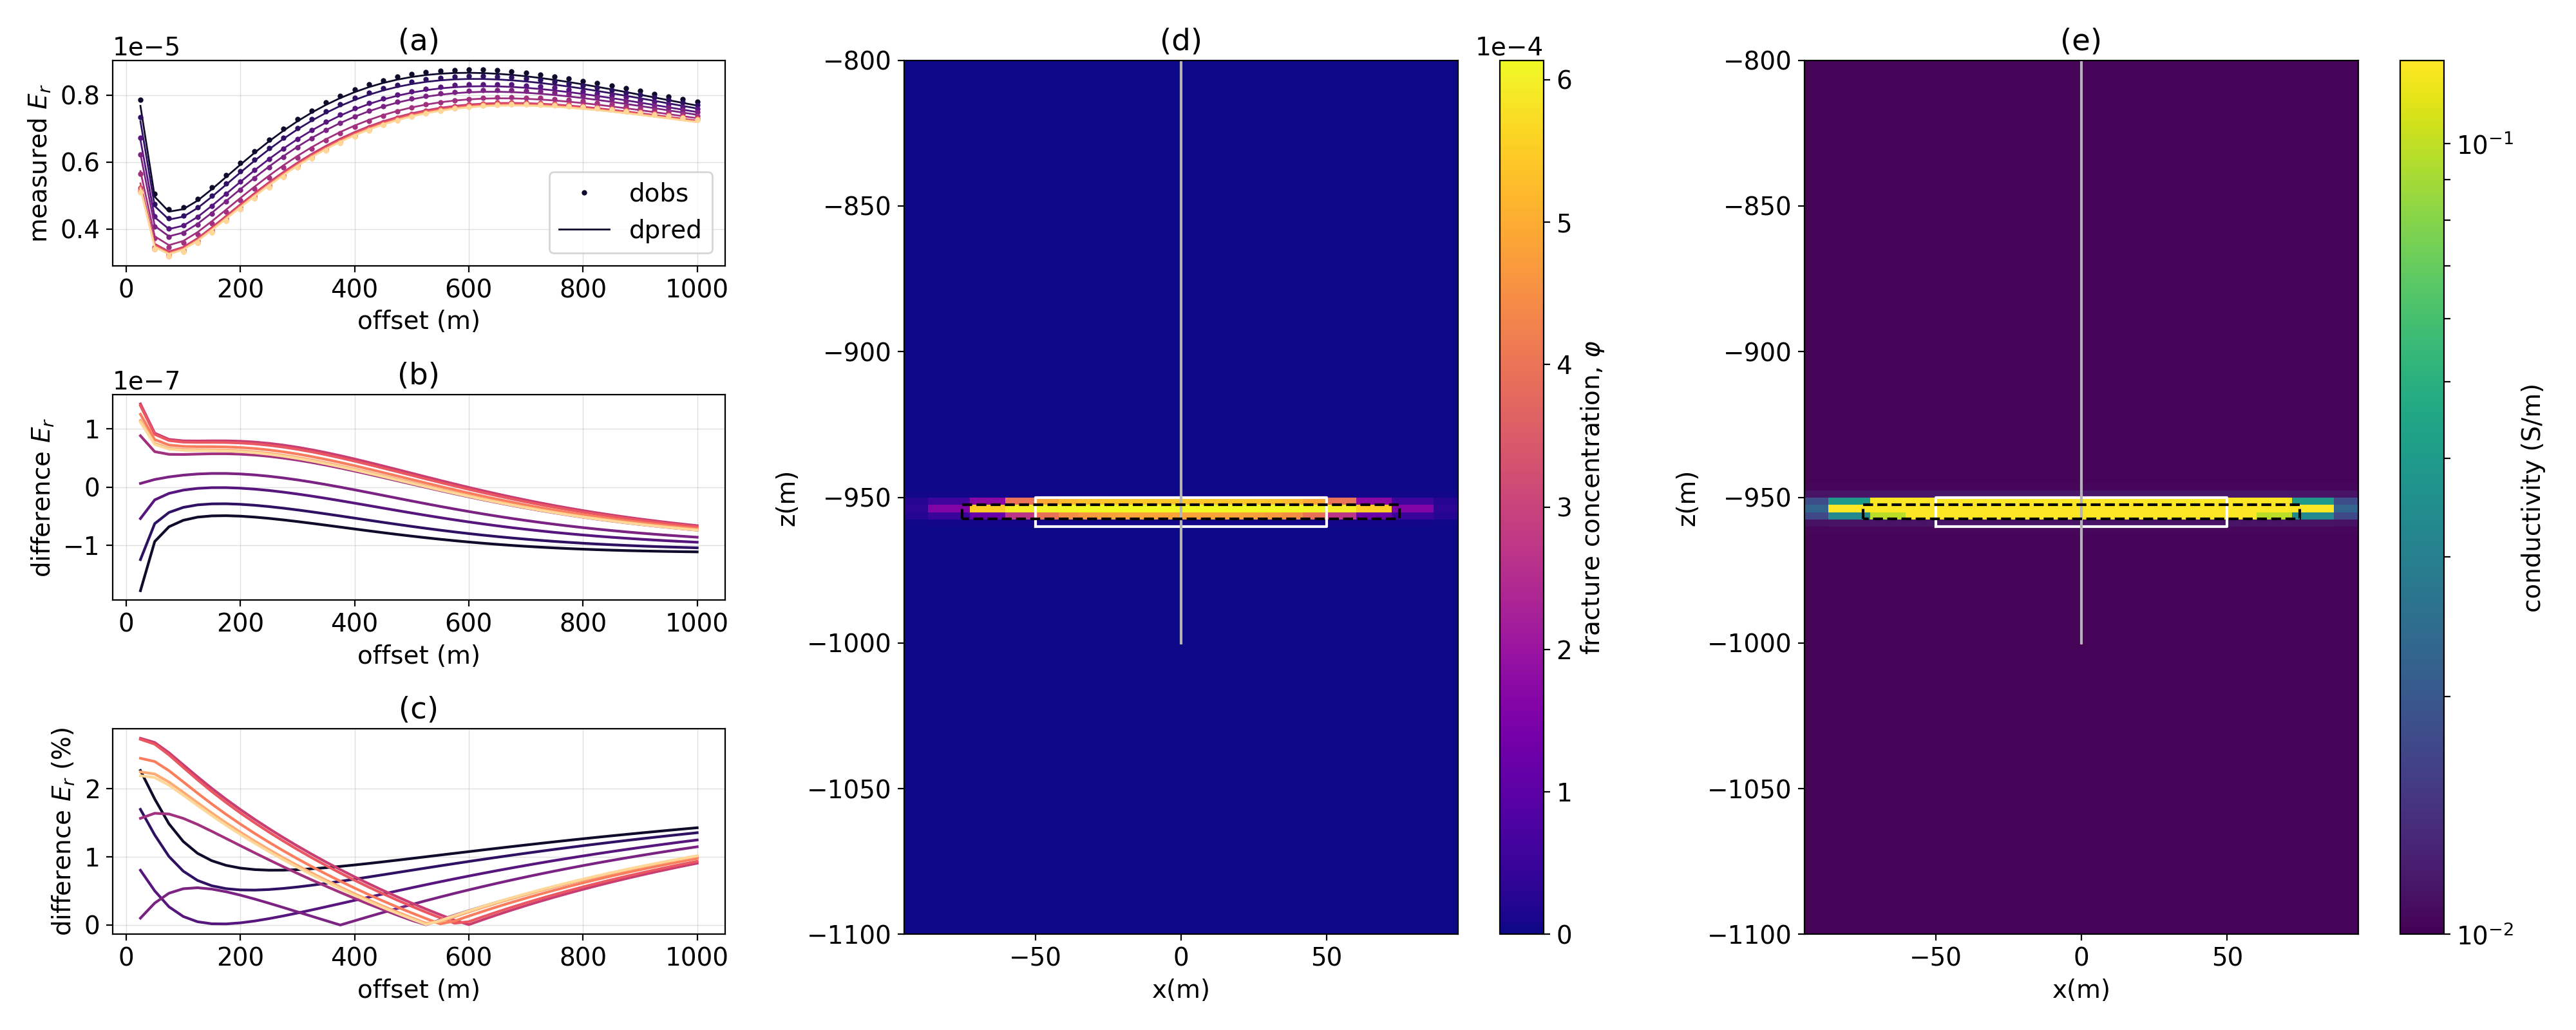
\includegraphics[width=\textwidth]{figures/inversion/dc_parametric_inversion_phi_vol_correctz0_large_r.png}
    \end{center}
\caption{
    Parametric inversion using effective medium theory and a volume data-misfit in the statement of the inverse problem.
    The uncertainty on the volume datum was 5\%. The starting model was the same as used in Figure \ref{fig:dc_parametric_inversion_phi_correctz0_large_r}
    The inversion reached a global $\chi$-factor $<$ 0.05 after 5 iterations.
}
\label{fig:dc_parametric_inversion_phi_vol_correctz0_large_r}
\end{figure}


\section{Conclusions}
The inversions shown in this section provide a glimpse into the nonuniqueness of the inverse problem, particularly when steel-cased wells are present. Pushing the voxel inversion allows us to estimate the depth-center of the fractures, however a smooth inversion provides diffuse structures by design and therefore is not particularly insightful for estimating the geometry of a compact target. Parametric inversions provide a strategy for obtaining a simple geometric structure from the inversion. A standard approach to the parametric inversion and inverting for log-conductivity of the target and the background proved to be quite unstable, and, in particular, the recovered conductivity varied by orders of magnitude depending on the starting model. I suspect that the high conductivity of the casing, which is electrically in contact with the target, plays a significant role in this instability. This could be further examined in a study which varies the conductivity of the casing. If the casing is indeed the main cause of the instability, then reducing the conductivity of the borehole should reduce the large fluctuations in the recovered conductivity of the target.

If instead of inverting for log-conductivity, we invert for fracture concentration using effective medium theory, the parametric inversion is much more stable. The effective medium theory mapping is an approximately linear relationship between the fracture concentration and the electrical conductivity, and it provides natural bounds on the recovered conductivity. Additionally, it allows us to incorporate a volume data-misfit term in the statement of the inverse problem. With the presented inversion approach, the mathematical statement of the effective medium theory relationship between fracture concentration electrical conductivity could be replaced by an empirical relationship based upon lab-studies. Although I used examples with a constant background, this is not required. A variable background model, based upon an inversion of data collected before the fracture, can be used.

Framing the inverse problem as one for fracture concentration resulted in a more robust inversion scheme that was less sensitive to the starting model, but clearly, there is significant non-uniqueness in the DC problem and we do not have much sensitivity to the geometry of the target. Experimentation shows that even adding vertical electric field data from an offset borehole does not significantly improve the results. Here is where electromagnetics has significant potential to provide further insights. In addition to the static excitation at DC, the time-variation of the fields causes induction processes and variation in the direction and magnitude of the fields, resulting in a richer data set. Chapter \ref{ch:casing-software} examined details of the physics of the induction process for conductive permeable wells. The next step, which is a topic of future research, is to combine those research results with the insight I have developed in this inversion chapter to quantify how much additional information can be obtained using the full EM data set.
